\RequirePackage{fix-cm}

\documentclass[
openright,
titlepage,
numbers=noenddot,
headinclude,
footinclude=true,
cleardoublepage=empty,
abstractoff,
BCOR=5mm,
paper=a4,
fontsize=12pt,
ngerman,
american,
oneside,
dottedtoc
]{scrreprt}

% ****************************************************************************************************
% classicthesis-config.tex 
% formerly known as loadpackages.sty, classicthesis-ldpkg.sty, and classicthesis-preamble.sty 
% Use it at the beginning of your ClassicThesis.tex, or as a LaTeX Preamble 
% in your ClassicThesis.{tex,lyx} with % ****************************************************************************************************
% classicthesis-config.tex 
% formerly known as loadpackages.sty, classicthesis-ldpkg.sty, and classicthesis-preamble.sty 
% Use it at the beginning of your ClassicThesis.tex, or as a LaTeX Preamble 
% in your ClassicThesis.{tex,lyx} with % ****************************************************************************************************
% classicthesis-config.tex 
% formerly known as loadpackages.sty, classicthesis-ldpkg.sty, and classicthesis-preamble.sty 
% Use it at the beginning of your ClassicThesis.tex, or as a LaTeX Preamble 
% in your ClassicThesis.{tex,lyx} with \input{classicthesis-config}
% ****************************************************************************************************  
% If you like the classicthesis, then I would appreciate a postcard. 
% My address can be found in the file ClassicThesis.pdf. A collection 
% of the postcards I received so far is available online at 
% http://postcards.miede.de
% ****************************************************************************************************


% ****************************************************************************************************
% 0. Set the encoding of your files. UTF-8 is the only sensible encoding nowadays. If you can't read
% äöüßáéçèê∂åëæƒÏ€ then change the encoding setting in your editor, not the line below. If your editor
% does not support utf8 use another editor!
% ****************************************************************************************************
\PassOptionsToPackage{utf8}{inputenc}
	\usepackage{inputenc}

% ****************************************************************************************************
% 1. Configure classicthesis for your needs here, e.g., remove "drafting" below 
% in order to deactivate the time-stamp on the pages
% ****************************************************************************************************
\PassOptionsToPackage{
eulerchapternumbers,
listings,
pdfspacing,
subfig,
beramono,
eulermath,
parts,
linedheaders
}{classicthesis}                                        

% ********************************************************************
% Available options for classicthesis.sty 
% (see ClassicThesis.pdf for more information):
% drafting
% parts nochapters linedheaders
% eulerchapternumbers beramono eulermath pdfspacing minionprospacing
% tocaligned dottedtoc manychapters
% listings floatperchapter subfig
% ********************************************************************


% ****************************************************************************************************
% 2. Personal data and user ad-hoc commands
% ****************************************************************************************************
\newcommand{\myTitle}{A Classic Thesis Style\xspace}
\newcommand{\mySubtitle}{An Homage to The Elements of Typographic Style\xspace}
\newcommand{\myDegree}{Doktor-Ingenieur (Dr.-Ing.)\xspace}
\newcommand{\myName}{André Miede\xspace}
\newcommand{\myProf}{Put name here\xspace}
\newcommand{\myOtherProf}{Put name here\xspace}
\newcommand{\mySupervisor}{Put name here\xspace}
\newcommand{\myFaculty}{Put data here\xspace}
\newcommand{\myDepartment}{Put data here\xspace}
\newcommand{\myUni}{Put data here\xspace}
\newcommand{\myLocation}{Saarbrücken\xspace}
\newcommand{\myTime}{September 2015\xspace}
\newcommand{\myVersion}{version 4.2\xspace}

% ********************************************************************
% Setup, finetuning, and useful commands
% ********************************************************************
\newcounter{dummy} % necessary for correct hyperlinks (to index, bib, etc.)
\newlength{\abcd} % for ab..z string length calculation
\providecommand{\mLyX}{L\kern-.1667em\lower.25em\hbox{Y}\kern-.125emX\@}
\newcommand{\ie}{i.\,e.}
\newcommand{\Ie}{I.\,e.}
\newcommand{\eg}{e.\,g.}
\newcommand{\Eg}{E.\,g.} 
% ****************************************************************************************************


% ****************************************************************************************************
% 3. Loading some handy packages
% ****************************************************************************************************
% ******************************************************************** 
% Packages with options that might require adjustments
% ******************************************************************** 
%\PassOptionsToPackage{ngerman,american}{babel}   % change this to your language(s)
% Spanish languages need extra options in order to work with this template
%\PassOptionsToPackage{spanish,es-lcroman}{babel}
	\usepackage{babel}                  

\usepackage{csquotes}
\PassOptionsToPackage{%
    %backend=biber, %instead of bibtex
	backend=bibtex8,bibencoding=ascii,%
	language=auto,%
	style=numeric-comp,%
    %style=authoryear-comp, % Author 1999, 2010
    %bibstyle=authoryear,dashed=false, % dashed: substitute rep. author with ---
    sorting=nyt, % name, year, title
    maxbibnames=10, % default: 3, et al.
    %backref=true,%
    natbib=true % natbib compatibility mode (\citep and \citet still work)
}{biblatex}
    \usepackage[sorting=none, backref]{biblatex} % citation in order of appearance + backref

\PassOptionsToPackage{fleqn}{amsmath}       % math environments and more by the AMS 
    \usepackage{amsmath}

% ******************************************************************** 
% General useful packages
% ******************************************************************** 
\PassOptionsToPackage{T1}{fontenc} % T2A for cyrillics
    \usepackage{fontenc}     
\usepackage{textcomp} % fix warning with missing font shapes
\usepackage{scrhack} % fix warnings when using KOMA with listings package          
\usepackage{xspace} % to get the spacing after macros right  
\usepackage{mparhack} % get marginpar right
\usepackage{fixltx2e} % fixes some LaTeX stuff --> since 2015 in the LaTeX kernel (see below)
%\usepackage[latest]{latexrelease} % will be used once available in more distributions (ISSUE #107)
\PassOptionsToPackage{printonlyused,smaller}{acronym} 
    \usepackage{acronym} % nice macros for handling all acronyms in the thesis
    %\renewcommand{\bflabel}[1]{{#1}\hfill} % fix the list of acronyms --> no longer working
    %\renewcommand*{\acsfont}[1]{\textsc{#1}} 
    \renewcommand*{\aclabelfont}[1]{\acsfont{#1}}
% ****************************************************************************************************


% ****************************************************************************************************
% 4. Setup floats: tables, (sub)figures, and captions
% ****************************************************************************************************
\usepackage{tabularx} % better tables
    \setlength{\extrarowheight}{3pt} % increase table row height
\newcommand{\tableheadline}[1]{\multicolumn{1}{c}{\spacedlowsmallcaps{#1}}}
\newcommand{\myfloatalign}{\centering} % to be used with each float for alignment
\usepackage{caption}
% Thanks to cgnieder and Claus Lahiri
% http://tex.stackexchange.com/questions/69349/spacedlowsmallcaps-in-caption-label
% [REMOVED DUE TO OTHER PROBLEMS, SEE ISSUE #82]    
%\DeclareCaptionLabelFormat{smallcaps}{\bothIfFirst{#1}{~}\MakeTextLowercase{\textsc{#2}}}
%\captionsetup{font=small,labelformat=smallcaps} % format=hang,
\captionsetup{font=small} % format=hang,
\usepackage{subfig}  
% ****************************************************************************************************


% ****************************************************************************************************
% 5. Setup code listings
% ****************************************************************************************************
\usepackage{listings} 
%\lstset{emph={trueIndex,root},emphstyle=\color{BlueViolet}}%\underbar} % for special keywords
\lstset{language=[LaTeX]Tex,%C++,
    morekeywords={PassOptionsToPackage,selectlanguage},
    keywordstyle=\color{RoyalBlue},%\bfseries,
    basicstyle=\small\ttfamily,
    %identifierstyle=\color{NavyBlue},
    commentstyle=\color{Green}\ttfamily,
    stringstyle=\rmfamily,
    numbers=none,%left,%
    numberstyle=\scriptsize,%\tiny
    stepnumber=5,
    numbersep=8pt,
    showstringspaces=false,
    breaklines=true,
    %frameround=ftff,
    %frame=single,
    belowcaptionskip=.75\baselineskip
    %frame=L
} 
% ****************************************************************************************************             


% ****************************************************************************************************
% 6. PDFLaTeX, hyperreferences and citation backreferences
% ****************************************************************************************************
% ********************************************************************
% Using PDFLaTeX
% ********************************************************************
\PassOptionsToPackage{pdftex,hyperfootnotes=false,pdfpagelabels}{hyperref}
    \usepackage{hyperref}  % backref linktocpage pagebackref
\pdfcompresslevel=9
\pdfadjustspacing=1 
\PassOptionsToPackage{pdftex}{graphicx}
    \usepackage{graphicx} 
 

% ********************************************************************
% Hyperreferences
% ********************************************************************
\hypersetup{%
    %draft, % = no hyperlinking at all (useful in b/w printouts)
    colorlinks=true, linktocpage=true, pdfstartpage=3, pdfstartview=FitV,%
    % uncomment the following line if you want to have black links (e.g., for printing)
    %colorlinks=false, linktocpage=false, pdfstartpage=3, pdfstartview=FitV, pdfborder={0 0 0},%
    breaklinks=true, pdfpagemode=UseNone, pageanchor=true, pdfpagemode=UseOutlines,%
    plainpages=false, bookmarksnumbered, bookmarksopen=true, bookmarksopenlevel=1,%
    hypertexnames=true, pdfhighlight=/O,%nesting=true,%frenchlinks,%
    urlcolor=webbrown, linkcolor=RoyalBlue, citecolor=webgreen, %pagecolor=RoyalBlue,%
    %urlcolor=Black, linkcolor=Black, citecolor=Black, %pagecolor=Black,%
    pdftitle={\myTitle},%
    pdfauthor={\textcopyright\ \myName, \myUni, \myFaculty},%
    pdfsubject={},%
    pdfkeywords={},%
    pdfcreator={pdfLaTeX},%
    pdfproducer={LaTeX with hyperref and classicthesis}%
}   

% ********************************************************************
% Setup autoreferences
% ********************************************************************
% There are some issues regarding autorefnames
% http://www.ureader.de/msg/136221647.aspx
% http://www.tex.ac.uk/cgi-bin/texfaq2html?label=latexwords
% you have to redefine the makros for the 
% language you use, e.g., american, ngerman
% (as chosen when loading babel/AtBeginDocument)
% ********************************************************************
\makeatletter
\@ifpackageloaded{babel}%
    {%
       \addto\extrasamerican{%
			\renewcommand*{\figureautorefname}{Figure}%
			\renewcommand*{\tableautorefname}{Table}%
			\renewcommand*{\partautorefname}{Part}%
			\renewcommand*{\chapterautorefname}{Chapter}%
			\renewcommand*{\sectionautorefname}{Section}%
			\renewcommand*{\subsectionautorefname}{Section}%
			\renewcommand*{\subsubsectionautorefname}{Section}%     
                }%
       \addto\extrasngerman{% 
			\renewcommand*{\paragraphautorefname}{Absatz}%
			\renewcommand*{\subparagraphautorefname}{Unterabsatz}%
			\renewcommand*{\footnoteautorefname}{Fu\"snote}%
			\renewcommand*{\FancyVerbLineautorefname}{Zeile}%
			\renewcommand*{\theoremautorefname}{Theorem}%
			\renewcommand*{\appendixautorefname}{Anhang}%
			\renewcommand*{\equationautorefname}{Gleichung}%        
			\renewcommand*{\itemautorefname}{Punkt}%
                }%  
            % Fix to getting autorefs for subfigures right (thanks to Belinda Vogt for changing the definition)
            \providecommand{\subfigureautorefname}{\figureautorefname}%             
    }{\relax}
\makeatother


% ****************************************************************************************************
% 7. Last calls before the bar closes
% ****************************************************************************************************
% ********************************************************************
% Development Stuff
% ********************************************************************
\listfiles
%\PassOptionsToPackage{l2tabu,orthodox,abort}{nag}
%   \usepackage{nag}
%\PassOptionsToPackage{warning, all}{onlyamsmath}
%   \usepackage{onlyamsmath}

% ********************************************************************
% Last, but not least...
% ********************************************************************
\usepackage{classicthesis} 
% ****************************************************************************************************


% ****************************************************************************************************
% 8. Further adjustments (experimental)
% ****************************************************************************************************
% ********************************************************************
% Changing the text area
% ********************************************************************
%\linespread{1.05} % a bit more for Palatino
%\areaset[current]{312pt}{761pt} % 686 (factor 2.2) + 33 head + 42 head \the\footskip
%\setlength{\marginparwidth}{7em}%
%\setlength{\marginparsep}{2em}%

% ********************************************************************
% Using different fonts
% ********************************************************************
%\usepackage[oldstylenums]{kpfonts} % oldstyle notextcomp
%\usepackage[osf]{libertine}
%\usepackage[light,condensed,math]{iwona}
%\renewcommand{\sfdefault}{iwona}
%\usepackage{lmodern} % <-- no osf support :-(
%\usepackage{cfr-lm} % 
%\usepackage[urw-garamond]{mathdesign} <-- no osf support :-(
%\usepackage[default,osfigures]{opensans} % scale=0.95 
%\usepackage[sfdefault]{FiraSans}
% ****************************************************************************************************

% ****************************************************************************************************  
% If you like the classicthesis, then I would appreciate a postcard. 
% My address can be found in the file ClassicThesis.pdf. A collection 
% of the postcards I received so far is available online at 
% http://postcards.miede.de
% ****************************************************************************************************


% ****************************************************************************************************
% 0. Set the encoding of your files. UTF-8 is the only sensible encoding nowadays. If you can't read
% äöüßáéçèê∂åëæƒÏ€ then change the encoding setting in your editor, not the line below. If your editor
% does not support utf8 use another editor!
% ****************************************************************************************************
\PassOptionsToPackage{utf8}{inputenc}
	\usepackage{inputenc}

% ****************************************************************************************************
% 1. Configure classicthesis for your needs here, e.g., remove "drafting" below 
% in order to deactivate the time-stamp on the pages
% ****************************************************************************************************
\PassOptionsToPackage{
eulerchapternumbers,
listings,
pdfspacing,
subfig,
beramono,
eulermath,
parts,
linedheaders
}{classicthesis}                                        

% ********************************************************************
% Available options for classicthesis.sty 
% (see ClassicThesis.pdf for more information):
% drafting
% parts nochapters linedheaders
% eulerchapternumbers beramono eulermath pdfspacing minionprospacing
% tocaligned dottedtoc manychapters
% listings floatperchapter subfig
% ********************************************************************


% ****************************************************************************************************
% 2. Personal data and user ad-hoc commands
% ****************************************************************************************************
\newcommand{\myTitle}{A Classic Thesis Style\xspace}
\newcommand{\mySubtitle}{An Homage to The Elements of Typographic Style\xspace}
\newcommand{\myDegree}{Doktor-Ingenieur (Dr.-Ing.)\xspace}
\newcommand{\myName}{André Miede\xspace}
\newcommand{\myProf}{Put name here\xspace}
\newcommand{\myOtherProf}{Put name here\xspace}
\newcommand{\mySupervisor}{Put name here\xspace}
\newcommand{\myFaculty}{Put data here\xspace}
\newcommand{\myDepartment}{Put data here\xspace}
\newcommand{\myUni}{Put data here\xspace}
\newcommand{\myLocation}{Saarbrücken\xspace}
\newcommand{\myTime}{September 2015\xspace}
\newcommand{\myVersion}{version 4.2\xspace}

% ********************************************************************
% Setup, finetuning, and useful commands
% ********************************************************************
\newcounter{dummy} % necessary for correct hyperlinks (to index, bib, etc.)
\newlength{\abcd} % for ab..z string length calculation
\providecommand{\mLyX}{L\kern-.1667em\lower.25em\hbox{Y}\kern-.125emX\@}
\newcommand{\ie}{i.\,e.}
\newcommand{\Ie}{I.\,e.}
\newcommand{\eg}{e.\,g.}
\newcommand{\Eg}{E.\,g.} 
% ****************************************************************************************************


% ****************************************************************************************************
% 3. Loading some handy packages
% ****************************************************************************************************
% ******************************************************************** 
% Packages with options that might require adjustments
% ******************************************************************** 
%\PassOptionsToPackage{ngerman,american}{babel}   % change this to your language(s)
% Spanish languages need extra options in order to work with this template
%\PassOptionsToPackage{spanish,es-lcroman}{babel}
	\usepackage{babel}                  

\usepackage{csquotes}
\PassOptionsToPackage{%
    %backend=biber, %instead of bibtex
	backend=bibtex8,bibencoding=ascii,%
	language=auto,%
	style=numeric-comp,%
    %style=authoryear-comp, % Author 1999, 2010
    %bibstyle=authoryear,dashed=false, % dashed: substitute rep. author with ---
    sorting=nyt, % name, year, title
    maxbibnames=10, % default: 3, et al.
    %backref=true,%
    natbib=true % natbib compatibility mode (\citep and \citet still work)
}{biblatex}
    \usepackage[sorting=none, backref]{biblatex} % citation in order of appearance + backref

\PassOptionsToPackage{fleqn}{amsmath}       % math environments and more by the AMS 
    \usepackage{amsmath}

% ******************************************************************** 
% General useful packages
% ******************************************************************** 
\PassOptionsToPackage{T1}{fontenc} % T2A for cyrillics
    \usepackage{fontenc}     
\usepackage{textcomp} % fix warning with missing font shapes
\usepackage{scrhack} % fix warnings when using KOMA with listings package          
\usepackage{xspace} % to get the spacing after macros right  
\usepackage{mparhack} % get marginpar right
\usepackage{fixltx2e} % fixes some LaTeX stuff --> since 2015 in the LaTeX kernel (see below)
%\usepackage[latest]{latexrelease} % will be used once available in more distributions (ISSUE #107)
\PassOptionsToPackage{printonlyused,smaller}{acronym} 
    \usepackage{acronym} % nice macros for handling all acronyms in the thesis
    %\renewcommand{\bflabel}[1]{{#1}\hfill} % fix the list of acronyms --> no longer working
    %\renewcommand*{\acsfont}[1]{\textsc{#1}} 
    \renewcommand*{\aclabelfont}[1]{\acsfont{#1}}
% ****************************************************************************************************


% ****************************************************************************************************
% 4. Setup floats: tables, (sub)figures, and captions
% ****************************************************************************************************
\usepackage{tabularx} % better tables
    \setlength{\extrarowheight}{3pt} % increase table row height
\newcommand{\tableheadline}[1]{\multicolumn{1}{c}{\spacedlowsmallcaps{#1}}}
\newcommand{\myfloatalign}{\centering} % to be used with each float for alignment
\usepackage{caption}
% Thanks to cgnieder and Claus Lahiri
% http://tex.stackexchange.com/questions/69349/spacedlowsmallcaps-in-caption-label
% [REMOVED DUE TO OTHER PROBLEMS, SEE ISSUE #82]    
%\DeclareCaptionLabelFormat{smallcaps}{\bothIfFirst{#1}{~}\MakeTextLowercase{\textsc{#2}}}
%\captionsetup{font=small,labelformat=smallcaps} % format=hang,
\captionsetup{font=small} % format=hang,
\usepackage{subfig}  
% ****************************************************************************************************


% ****************************************************************************************************
% 5. Setup code listings
% ****************************************************************************************************
\usepackage{listings} 
%\lstset{emph={trueIndex,root},emphstyle=\color{BlueViolet}}%\underbar} % for special keywords
\lstset{language=[LaTeX]Tex,%C++,
    morekeywords={PassOptionsToPackage,selectlanguage},
    keywordstyle=\color{RoyalBlue},%\bfseries,
    basicstyle=\small\ttfamily,
    %identifierstyle=\color{NavyBlue},
    commentstyle=\color{Green}\ttfamily,
    stringstyle=\rmfamily,
    numbers=none,%left,%
    numberstyle=\scriptsize,%\tiny
    stepnumber=5,
    numbersep=8pt,
    showstringspaces=false,
    breaklines=true,
    %frameround=ftff,
    %frame=single,
    belowcaptionskip=.75\baselineskip
    %frame=L
} 
% ****************************************************************************************************             


% ****************************************************************************************************
% 6. PDFLaTeX, hyperreferences and citation backreferences
% ****************************************************************************************************
% ********************************************************************
% Using PDFLaTeX
% ********************************************************************
\PassOptionsToPackage{pdftex,hyperfootnotes=false,pdfpagelabels}{hyperref}
    \usepackage{hyperref}  % backref linktocpage pagebackref
\pdfcompresslevel=9
\pdfadjustspacing=1 
\PassOptionsToPackage{pdftex}{graphicx}
    \usepackage{graphicx} 
 

% ********************************************************************
% Hyperreferences
% ********************************************************************
\hypersetup{%
    %draft, % = no hyperlinking at all (useful in b/w printouts)
    colorlinks=true, linktocpage=true, pdfstartpage=3, pdfstartview=FitV,%
    % uncomment the following line if you want to have black links (e.g., for printing)
    %colorlinks=false, linktocpage=false, pdfstartpage=3, pdfstartview=FitV, pdfborder={0 0 0},%
    breaklinks=true, pdfpagemode=UseNone, pageanchor=true, pdfpagemode=UseOutlines,%
    plainpages=false, bookmarksnumbered, bookmarksopen=true, bookmarksopenlevel=1,%
    hypertexnames=true, pdfhighlight=/O,%nesting=true,%frenchlinks,%
    urlcolor=webbrown, linkcolor=RoyalBlue, citecolor=webgreen, %pagecolor=RoyalBlue,%
    %urlcolor=Black, linkcolor=Black, citecolor=Black, %pagecolor=Black,%
    pdftitle={\myTitle},%
    pdfauthor={\textcopyright\ \myName, \myUni, \myFaculty},%
    pdfsubject={},%
    pdfkeywords={},%
    pdfcreator={pdfLaTeX},%
    pdfproducer={LaTeX with hyperref and classicthesis}%
}   

% ********************************************************************
% Setup autoreferences
% ********************************************************************
% There are some issues regarding autorefnames
% http://www.ureader.de/msg/136221647.aspx
% http://www.tex.ac.uk/cgi-bin/texfaq2html?label=latexwords
% you have to redefine the makros for the 
% language you use, e.g., american, ngerman
% (as chosen when loading babel/AtBeginDocument)
% ********************************************************************
\makeatletter
\@ifpackageloaded{babel}%
    {%
       \addto\extrasamerican{%
			\renewcommand*{\figureautorefname}{Figure}%
			\renewcommand*{\tableautorefname}{Table}%
			\renewcommand*{\partautorefname}{Part}%
			\renewcommand*{\chapterautorefname}{Chapter}%
			\renewcommand*{\sectionautorefname}{Section}%
			\renewcommand*{\subsectionautorefname}{Section}%
			\renewcommand*{\subsubsectionautorefname}{Section}%     
                }%
       \addto\extrasngerman{% 
			\renewcommand*{\paragraphautorefname}{Absatz}%
			\renewcommand*{\subparagraphautorefname}{Unterabsatz}%
			\renewcommand*{\footnoteautorefname}{Fu\"snote}%
			\renewcommand*{\FancyVerbLineautorefname}{Zeile}%
			\renewcommand*{\theoremautorefname}{Theorem}%
			\renewcommand*{\appendixautorefname}{Anhang}%
			\renewcommand*{\equationautorefname}{Gleichung}%        
			\renewcommand*{\itemautorefname}{Punkt}%
                }%  
            % Fix to getting autorefs for subfigures right (thanks to Belinda Vogt for changing the definition)
            \providecommand{\subfigureautorefname}{\figureautorefname}%             
    }{\relax}
\makeatother


% ****************************************************************************************************
% 7. Last calls before the bar closes
% ****************************************************************************************************
% ********************************************************************
% Development Stuff
% ********************************************************************
\listfiles
%\PassOptionsToPackage{l2tabu,orthodox,abort}{nag}
%   \usepackage{nag}
%\PassOptionsToPackage{warning, all}{onlyamsmath}
%   \usepackage{onlyamsmath}

% ********************************************************************
% Last, but not least...
% ********************************************************************
\usepackage{classicthesis} 
% ****************************************************************************************************


% ****************************************************************************************************
% 8. Further adjustments (experimental)
% ****************************************************************************************************
% ********************************************************************
% Changing the text area
% ********************************************************************
%\linespread{1.05} % a bit more for Palatino
%\areaset[current]{312pt}{761pt} % 686 (factor 2.2) + 33 head + 42 head \the\footskip
%\setlength{\marginparwidth}{7em}%
%\setlength{\marginparsep}{2em}%

% ********************************************************************
% Using different fonts
% ********************************************************************
%\usepackage[oldstylenums]{kpfonts} % oldstyle notextcomp
%\usepackage[osf]{libertine}
%\usepackage[light,condensed,math]{iwona}
%\renewcommand{\sfdefault}{iwona}
%\usepackage{lmodern} % <-- no osf support :-(
%\usepackage{cfr-lm} % 
%\usepackage[urw-garamond]{mathdesign} <-- no osf support :-(
%\usepackage[default,osfigures]{opensans} % scale=0.95 
%\usepackage[sfdefault]{FiraSans}
% ****************************************************************************************************

% ****************************************************************************************************  
% If you like the classicthesis, then I would appreciate a postcard. 
% My address can be found in the file ClassicThesis.pdf. A collection 
% of the postcards I received so far is available online at 
% http://postcards.miede.de
% ****************************************************************************************************


% ****************************************************************************************************
% 0. Set the encoding of your files. UTF-8 is the only sensible encoding nowadays. If you can't read
% äöüßáéçèê∂åëæƒÏ€ then change the encoding setting in your editor, not the line below. If your editor
% does not support utf8 use another editor!
% ****************************************************************************************************
\PassOptionsToPackage{utf8}{inputenc}
	\usepackage{inputenc}

% ****************************************************************************************************
% 1. Configure classicthesis for your needs here, e.g., remove "drafting" below 
% in order to deactivate the time-stamp on the pages
% ****************************************************************************************************
\PassOptionsToPackage{
eulerchapternumbers,
listings,
pdfspacing,
subfig,
beramono,
eulermath,
parts,
linedheaders
}{classicthesis}                                        

% ********************************************************************
% Available options for classicthesis.sty 
% (see ClassicThesis.pdf for more information):
% drafting
% parts nochapters linedheaders
% eulerchapternumbers beramono eulermath pdfspacing minionprospacing
% tocaligned dottedtoc manychapters
% listings floatperchapter subfig
% ********************************************************************


% ****************************************************************************************************
% 2. Personal data and user ad-hoc commands
% ****************************************************************************************************
\newcommand{\myTitle}{A Classic Thesis Style\xspace}
\newcommand{\mySubtitle}{An Homage to The Elements of Typographic Style\xspace}
\newcommand{\myDegree}{Doktor-Ingenieur (Dr.-Ing.)\xspace}
\newcommand{\myName}{André Miede\xspace}
\newcommand{\myProf}{Put name here\xspace}
\newcommand{\myOtherProf}{Put name here\xspace}
\newcommand{\mySupervisor}{Put name here\xspace}
\newcommand{\myFaculty}{Put data here\xspace}
\newcommand{\myDepartment}{Put data here\xspace}
\newcommand{\myUni}{Put data here\xspace}
\newcommand{\myLocation}{Saarbrücken\xspace}
\newcommand{\myTime}{September 2015\xspace}
\newcommand{\myVersion}{version 4.2\xspace}

% ********************************************************************
% Setup, finetuning, and useful commands
% ********************************************************************
\newcounter{dummy} % necessary for correct hyperlinks (to index, bib, etc.)
\newlength{\abcd} % for ab..z string length calculation
\providecommand{\mLyX}{L\kern-.1667em\lower.25em\hbox{Y}\kern-.125emX\@}
\newcommand{\ie}{i.\,e.}
\newcommand{\Ie}{I.\,e.}
\newcommand{\eg}{e.\,g.}
\newcommand{\Eg}{E.\,g.} 
% ****************************************************************************************************


% ****************************************************************************************************
% 3. Loading some handy packages
% ****************************************************************************************************
% ******************************************************************** 
% Packages with options that might require adjustments
% ******************************************************************** 
%\PassOptionsToPackage{ngerman,american}{babel}   % change this to your language(s)
% Spanish languages need extra options in order to work with this template
%\PassOptionsToPackage{spanish,es-lcroman}{babel}
	\usepackage{babel}                  

\usepackage{csquotes}
\PassOptionsToPackage{%
    %backend=biber, %instead of bibtex
	backend=bibtex8,bibencoding=ascii,%
	language=auto,%
	style=numeric-comp,%
    %style=authoryear-comp, % Author 1999, 2010
    %bibstyle=authoryear,dashed=false, % dashed: substitute rep. author with ---
    sorting=nyt, % name, year, title
    maxbibnames=10, % default: 3, et al.
    %backref=true,%
    natbib=true % natbib compatibility mode (\citep and \citet still work)
}{biblatex}
    \usepackage[sorting=none, backref]{biblatex} % citation in order of appearance + backref

\PassOptionsToPackage{fleqn}{amsmath}       % math environments and more by the AMS 
    \usepackage{amsmath}

% ******************************************************************** 
% General useful packages
% ******************************************************************** 
\PassOptionsToPackage{T1}{fontenc} % T2A for cyrillics
    \usepackage{fontenc}     
\usepackage{textcomp} % fix warning with missing font shapes
\usepackage{scrhack} % fix warnings when using KOMA with listings package          
\usepackage{xspace} % to get the spacing after macros right  
\usepackage{mparhack} % get marginpar right
\usepackage{fixltx2e} % fixes some LaTeX stuff --> since 2015 in the LaTeX kernel (see below)
%\usepackage[latest]{latexrelease} % will be used once available in more distributions (ISSUE #107)
\PassOptionsToPackage{printonlyused,smaller}{acronym} 
    \usepackage{acronym} % nice macros for handling all acronyms in the thesis
    %\renewcommand{\bflabel}[1]{{#1}\hfill} % fix the list of acronyms --> no longer working
    %\renewcommand*{\acsfont}[1]{\textsc{#1}} 
    \renewcommand*{\aclabelfont}[1]{\acsfont{#1}}
% ****************************************************************************************************


% ****************************************************************************************************
% 4. Setup floats: tables, (sub)figures, and captions
% ****************************************************************************************************
\usepackage{tabularx} % better tables
    \setlength{\extrarowheight}{3pt} % increase table row height
\newcommand{\tableheadline}[1]{\multicolumn{1}{c}{\spacedlowsmallcaps{#1}}}
\newcommand{\myfloatalign}{\centering} % to be used with each float for alignment
\usepackage{caption}
% Thanks to cgnieder and Claus Lahiri
% http://tex.stackexchange.com/questions/69349/spacedlowsmallcaps-in-caption-label
% [REMOVED DUE TO OTHER PROBLEMS, SEE ISSUE #82]    
%\DeclareCaptionLabelFormat{smallcaps}{\bothIfFirst{#1}{~}\MakeTextLowercase{\textsc{#2}}}
%\captionsetup{font=small,labelformat=smallcaps} % format=hang,
\captionsetup{font=small} % format=hang,
\usepackage{subfig}  
% ****************************************************************************************************


% ****************************************************************************************************
% 5. Setup code listings
% ****************************************************************************************************
\usepackage{listings} 
%\lstset{emph={trueIndex,root},emphstyle=\color{BlueViolet}}%\underbar} % for special keywords
\lstset{language=[LaTeX]Tex,%C++,
    morekeywords={PassOptionsToPackage,selectlanguage},
    keywordstyle=\color{RoyalBlue},%\bfseries,
    basicstyle=\small\ttfamily,
    %identifierstyle=\color{NavyBlue},
    commentstyle=\color{Green}\ttfamily,
    stringstyle=\rmfamily,
    numbers=none,%left,%
    numberstyle=\scriptsize,%\tiny
    stepnumber=5,
    numbersep=8pt,
    showstringspaces=false,
    breaklines=true,
    %frameround=ftff,
    %frame=single,
    belowcaptionskip=.75\baselineskip
    %frame=L
} 
% ****************************************************************************************************             


% ****************************************************************************************************
% 6. PDFLaTeX, hyperreferences and citation backreferences
% ****************************************************************************************************
% ********************************************************************
% Using PDFLaTeX
% ********************************************************************
\PassOptionsToPackage{pdftex,hyperfootnotes=false,pdfpagelabels}{hyperref}
    \usepackage{hyperref}  % backref linktocpage pagebackref
\pdfcompresslevel=9
\pdfadjustspacing=1 
\PassOptionsToPackage{pdftex}{graphicx}
    \usepackage{graphicx} 
 

% ********************************************************************
% Hyperreferences
% ********************************************************************
\hypersetup{%
    %draft, % = no hyperlinking at all (useful in b/w printouts)
    colorlinks=true, linktocpage=true, pdfstartpage=3, pdfstartview=FitV,%
    % uncomment the following line if you want to have black links (e.g., for printing)
    %colorlinks=false, linktocpage=false, pdfstartpage=3, pdfstartview=FitV, pdfborder={0 0 0},%
    breaklinks=true, pdfpagemode=UseNone, pageanchor=true, pdfpagemode=UseOutlines,%
    plainpages=false, bookmarksnumbered, bookmarksopen=true, bookmarksopenlevel=1,%
    hypertexnames=true, pdfhighlight=/O,%nesting=true,%frenchlinks,%
    urlcolor=webbrown, linkcolor=RoyalBlue, citecolor=webgreen, %pagecolor=RoyalBlue,%
    %urlcolor=Black, linkcolor=Black, citecolor=Black, %pagecolor=Black,%
    pdftitle={\myTitle},%
    pdfauthor={\textcopyright\ \myName, \myUni, \myFaculty},%
    pdfsubject={},%
    pdfkeywords={},%
    pdfcreator={pdfLaTeX},%
    pdfproducer={LaTeX with hyperref and classicthesis}%
}   

% ********************************************************************
% Setup autoreferences
% ********************************************************************
% There are some issues regarding autorefnames
% http://www.ureader.de/msg/136221647.aspx
% http://www.tex.ac.uk/cgi-bin/texfaq2html?label=latexwords
% you have to redefine the makros for the 
% language you use, e.g., american, ngerman
% (as chosen when loading babel/AtBeginDocument)
% ********************************************************************
\makeatletter
\@ifpackageloaded{babel}%
    {%
       \addto\extrasamerican{%
			\renewcommand*{\figureautorefname}{Figure}%
			\renewcommand*{\tableautorefname}{Table}%
			\renewcommand*{\partautorefname}{Part}%
			\renewcommand*{\chapterautorefname}{Chapter}%
			\renewcommand*{\sectionautorefname}{Section}%
			\renewcommand*{\subsectionautorefname}{Section}%
			\renewcommand*{\subsubsectionautorefname}{Section}%     
                }%
       \addto\extrasngerman{% 
			\renewcommand*{\paragraphautorefname}{Absatz}%
			\renewcommand*{\subparagraphautorefname}{Unterabsatz}%
			\renewcommand*{\footnoteautorefname}{Fu\"snote}%
			\renewcommand*{\FancyVerbLineautorefname}{Zeile}%
			\renewcommand*{\theoremautorefname}{Theorem}%
			\renewcommand*{\appendixautorefname}{Anhang}%
			\renewcommand*{\equationautorefname}{Gleichung}%        
			\renewcommand*{\itemautorefname}{Punkt}%
                }%  
            % Fix to getting autorefs for subfigures right (thanks to Belinda Vogt for changing the definition)
            \providecommand{\subfigureautorefname}{\figureautorefname}%             
    }{\relax}
\makeatother


% ****************************************************************************************************
% 7. Last calls before the bar closes
% ****************************************************************************************************
% ********************************************************************
% Development Stuff
% ********************************************************************
\listfiles
%\PassOptionsToPackage{l2tabu,orthodox,abort}{nag}
%   \usepackage{nag}
%\PassOptionsToPackage{warning, all}{onlyamsmath}
%   \usepackage{onlyamsmath}

% ********************************************************************
% Last, but not least...
% ********************************************************************
\usepackage{classicthesis} 
% ****************************************************************************************************


% ****************************************************************************************************
% 8. Further adjustments (experimental)
% ****************************************************************************************************
% ********************************************************************
% Changing the text area
% ********************************************************************
%\linespread{1.05} % a bit more for Palatino
%\areaset[current]{312pt}{761pt} % 686 (factor 2.2) + 33 head + 42 head \the\footskip
%\setlength{\marginparwidth}{7em}%
%\setlength{\marginparsep}{2em}%

% ********************************************************************
% Using different fonts
% ********************************************************************
%\usepackage[oldstylenums]{kpfonts} % oldstyle notextcomp
%\usepackage[osf]{libertine}
%\usepackage[light,condensed,math]{iwona}
%\renewcommand{\sfdefault}{iwona}
%\usepackage{lmodern} % <-- no osf support :-(
%\usepackage{cfr-lm} % 
%\usepackage[urw-garamond]{mathdesign} <-- no osf support :-(
%\usepackage[default,osfigures]{opensans} % scale=0.95 
%\usepackage[sfdefault]{FiraSans}
% ****************************************************************************************************


\usepackage[left=1in,right=1in,top=1in,bottom=1in]{geometry}

\addbibresource{Bibliography.bib}

\usepackage{microtype}

\captionsetup[figure]{labelfont=bf}

\setcounter{MaxMatrixCols}{12} % 12 states

\interfootnotelinepenalty=10000

\DefineBibliographyStrings{english}{ % rename backref
  backrefpage={cit. a p.},
  backrefpages={cit. a pp.}
}

\usepackage{float}

\usepackage{accents} % derivative dot bigger
\newcommand*{\dt}[1]{%
  \accentset{\mbox{\large\bfseries .}}{#1}}
\newcommand*{\ddt}[1]{%
  \accentset{\mbox{\large\bfseries .\hspace{-0.25ex}.}}{#1}}

\usepackage{xcolor}
%New colors defined below
\definecolor{codegreen}{rgb}{0,0.6,0}
\definecolor{codegray}{rgb}{0.5,0.5,0.5}
\definecolor{codepurple}{rgb}{0.58,0,0.82}
\definecolor{backcolour}{rgb}{0.95,0.95,0.92}
%Code listing style named "mystyle"
\lstdefinestyle{mystyle}{
  backgroundcolor=\color{backcolour}, commentstyle=\color{codegreen},
  keywordstyle=\color{magenta},
  numberstyle=\tiny\color{codegray},
  stringstyle=\color{codepurple},
  basicstyle=\ttfamily\footnotesize,
  breakatwhitespace=false,         
  breaklines=true,                 
  captionpos=b,                    
  keepspaces=true,                 
  numbers=left,                    
  numbersep=5pt,                  
  showspaces=false,                
  showstringspaces=false,
  showtabs=false,                  
  tabsize=2
}
%"mystyle" code listing set
\lstset{style=mystyle}

\usepackage{setspace}
\onehalfspacing

\usepackage{chngcntr}
\counterwithin{figure}{chapter}

\usepackage{graphicx}
\usepackage{epstopdf}

\begin{document}

\frenchspacing
\raggedbottom
\selectlanguage{american}
\pagenumbering{roman}
\pagestyle{plain}

\renewcommand{\contentsname}{Indice} % rename ToC
\renewcommand{\listfigurename}{Lista delle Figure} % rename LoF
\renewcommand{\listtablename}{Lista delle Tabelle} % rename LoT
\renewcommand{\lstlistlistingname}{Lista dei Codici} % rename LoL
\renewcommand{\bibname}{Bibliografia e Sitografia} % rename bib
\renewcommand{\figurename}{Figura} % rename fig
\renewcommand{\cftfigpresnum}{Figura } % rename fig inside LoF

% FRONT
% TITLE PAGE

\begin{titlepage}
   
\begin{spacing}{1}
	\begin{figure}[!htb]
    	\centering
    	
\includegraphics[keepaspectratio=true,scale=0.13]{gfx/logo_unipg}
	\end{figure}

	\begin{center}
    	\normalsize{UNIVERSITÀ DEGLI STUDI DI PERUGIA}
    	\vspace{5mm}
    	\\ \normalsize{DIPARTIMENTO DI INGEGNERIA}
    	\vspace{5mm}
    	\\ \small{Corso di Laurea Triennale in}
    	\vspace{5mm}
    	\\ \normalsize{INGEGNERIA INFORMATICA ED ELETTRONICA}
	\end{center}

	\vspace{15mm}
	
	\begin{center}
    	{\Large{\bf Studio e identificazione di modelli per la dinamica di un quadrirotore}}
	\end{center}
	
	\vspace{30mm}

	\begin{minipage}[t]{0.47\textwidth}
		{\large{Relatore:}{\large\vspace{3mm} \bf\\ \large{Prof. Paolo Valigi\\ }}}
		
		\vspace{1mm}
		
		{\large{Correlatore:}{\large\vspace{3mm} \bf\\ \large{Ing. Mirko Leomanni\\ }}}
	\end{minipage}
	\hfill
	\begin{minipage}[t]{0.47\textwidth}\raggedleft
		{\large{Candidato:}{\large\vspace{3mm} \bf\\ \large{Giovanni Versiglioni\\ }}}
	\end{minipage}

	\vspace{45mm}
	
	\hrulefill
	\\\centering{\normalsize{ANNO ACCADEMICO 2022/2023}}
\end{spacing}

\end{titlepage}
      
\newpage
\
\newpage
\cleardoublepage% DEDICATION

\thispagestyle{empty}
\refstepcounter{dummy}
\pdfbookmark[1]{Dedication}{Dedication}

\vspace*{3cm}

\begin{center}
    dedication
\end{center}

% \medskip

% \begin{center}
    % another dedication
% \end{center}

\newpage
\
\newpage
\pagestyle{scrheadings}
\cleardoublepage% SOMMARIO

\chapter*{Sommario}\label{ch:sommario}
Il quadrirotore è la piattaforma aerea maggiormente utilizzata ai fini di ricerca sui velivoli autonomi per la sue caratteristiche dinamiche che gli conferiscono un'ottima manovrabilità. Inoltre, sebbene sia instabile a ciclo aperto (come la maggior parte dei velivoli ad ala rotante), il quadrirotore mostra un buon grado di disaccoppiamento, cioè l'azione su uno dei segnali di controllo influisce quasi esclusivamente sul corrispondente grado di libertà.\\

La crescente complessità dei sistemi di controllo per questo tipo di mezzi necessita di modelli matematici estremamente accurati per la progettazione e la simulazione di relative leggi di controllo.\\

Lo scopo della seguente tesi è duplice. Il primo è quello di presentare un modello matematico che descriva rigorosamente la dinamica di un quadrirotore. Il secondo è quello di identificare un modello sufficientemente accurato per via sperimentale secondo un approccio a scatola nera, cioè esclusivamente sulla conoscenza di dati input-output. Nello specifico, sfruttando la proprietà di disaccoppiamento, si cercherà di identificare delle funzioni di trasferimento tempo continue in grado di descrivere il movimento del drone longitudinale, laterale e verticale (cioè lungo gli assi principali).\\

\textbf{Parole Chiave} \hspace{3mm} \textit{Unmanned Aerial Vehicle, Quadcopter, Quaternion, Robot Operating System, Gazebo, ArduCopter, MAVROS, System Identification, Black Box}

\cleardoublepage% TABLE OF CONTENTS

\refstepcounter{dummy}
\pdfbookmark[1]{\contentsname}{tableofcontents}
\setcounter{tocdepth}{2}
\setcounter{secnumdepth}{3}
\manualmark
\markboth{\spacedlowsmallcaps{\contentsname}}{\spacedlowsmallcaps{\contentsname}}
\tableofcontents 
\automark[section]{chapter}
\renewcommand{\chaptermark}[1]{\markboth{\spacedlowsmallcaps{#1}}{\spacedlowsmallcaps{#1}}}
\renewcommand{\sectionmark}[1]{\markright{\thesection\enspace\spacedlowsmallcaps{#1}}}

\clearpage

\begingroup 

    \let\clearpage\relax
    \let\cleardoublepage\relax
    \let\cleardoublepage\relax
    
    % LIST OF FIGURES
    \refstepcounter{dummy}
    \pdfbookmark[1]{\listfigurename}{lof}
    \listoffigures

    \pagebreak

	% LIST OF TABLES
    % \refstepcounter{dummy}
    % \pdfbookmark[1]{\listtablename}{lot}
    % \listoftables
        
    % \pagebreak
    
    % LIST OF LISTINGS
    % \refstepcounter{dummy}
    % \pdfbookmark[1]{\lstlistlistingname}{lol}
    % \lstlistoflistings 

    % \vspace{8ex}
       
    % ACRONYMS
    \refstepcounter{dummy}
    \pdfbookmark[1]{Acronyms}{acronyms}
    \markboth{\spacedlowsmallcaps{Acronyms}}{\spacedlowsmallcaps{Acronyms}}
    \chapter*{Acronimi} % rename acro
    \begin{acronym}[UMLX]
    	\acro{AGV}{Automated Guided Vehicle}
    	\acro{AMR}{Autonomous Mobile Robot}
    	\acro{UAV}{Unmanned Aerial Vehicle}
    	\acro{DoF}{Degree of Freedom}
    	\acro{LTP}{Local Tangent Plane}
    	\acro{ENU}{East North Up}
    	\acro{NED}{North East Down}
    	\acro{ABC}{Aircraft Body Center}
    	\acro{DCM}{Direct Cosine Matrix}
    	\acro{ROS}{Robot Operating System}
    	\acro{API}{Application Programming Interface}
    	\acro{DNS}{Domain Name System}
    	\acro{RPC}{Remote Procedure Call}
    	\acro{SLERP}{Spherical Linear Interpolation}
        \acro{RViz}{ROS Visualization}
        \acro{SITL}{Software In The Loop}
    	\acro{SISO}{Single Input Single Output}
    	\acro{MIMO}{Multi Input Multi Output}
    	\acro{LTI}{Linear Time Invariant}
    	\acro{NRMSE}{Normalized Root Mean Square Error}
    \end{acronym}  
                       
\endgroup


% MAIN
\cleardoublepage\pagenumbering{arabic}
% CHAPTER 1

\chapter{Introduzione}\label{ch:intro}
Nell'ultimo decennio l'industria robotica è cresciuta anno dopo anno, assumendo un ruolo decisivo nel più ampio campo dell'industria tecnologica. Secondo il rapporto "State of the robotics market" condotto da ABI Research \cite{ABI}, nel 2018 l'investimento totale nel settore della robotica è stato di circa 4 miliardi di dollari (US\$).\\

In particolare, la robotica mobile rappresenta uno dei trend maggiormente in crescita, con i veicoli a guida automatica - \ac{AGV} - che ne rappresentano un ruolo chiave nel mercato. Questi ultimi sono utilizzati principalmente in campo industriale per la movimentazione di prodotti all'interno di uno stabilimento. Tra le aziende leader di questo mercato primeggia Amazon, con investimenti continui volti a migliorare la produttività dei propri centri di distribuzione.\\

ABI sostiene che nel prossimo futuro gli \acs{AGV} continueranno ad avere un ruolo chiave nel settore della robotica mobile, ma prevede che i robot mobili autonomi - \ac{AMR} - li supereranno (in numero) entro il 2030. Questa ultima tipologia di robot mobili è caratterizzata da automi in grado di comprendere e spostarsi nell'ambiente esterno senza essere gestiti direttamente da un operatore.\\

In questo contesto, gli aeromobili a pilotaggio remoto - \ac{UAV} o droni - rappresentano un settore in via di sviluppo e trovano riscontro in un numero crescente di applicazioni: dal settore militare al settore civile, dal settore commerciale al settore dell'intrattenimento.

% NOTA: AGGIUNGERE INFO/ESEMPI AGV, AMR, UAV

\pagebreak

\section*{Breve Sommario}
L'elaborato si articola nei seguenti cinque capitoli:
\begin{itemize}
	\item \textbf{Capitolo 1} introduce la robotica mobile e le relative classificazioni
	\item \textbf{Capitolo 2} espone nel dettaglio la classe dei droni (\acs{UAV}), quindi descrive il modello fisico-matematico e il controllo di un quadrirotore 
	\item \textbf{Capitolo 3} introduce \acs{ROS} e ne spiega il funzionamento entrando nel dettaglio dei vari livelli che lo costituiscono, quindi descrive l'architettura utilizzata per simulare il volo di un quadrirotore
	\item \textbf{Capitolo 4} riporta le simulazioni di volo effettuate e i relativi dati input-output registrati, quindi spiega il procedimento seguito per ottenere modelli matematici \acs{SISO} che legano gli ingressi e le uscite fortemente dipendenti tra loro (e.g. rollio e posizione lungo y, beccheggio e posizione lungo x, spinta e posizione lungo z)
	\item \textbf{Capitolo 5} discute i risultati ottenuti e presenta eventuali sviluppi futuri
\end{itemize}

% CHAPTER 2

\chapter{UAV}\label{ch:uav}
Un aeromobile a pilotaggio remoto (\acs{UAV}) è un velivolo caratterizzato dall'assenza di un pilota umano a bordo. Il suo volo può essere controllato da un computer a bordo del mezzo oppure da remoto, seguendo i comandi di un pilota a terra.

% ------------------------------ CLASSIFICAZIONE ------------------------------

\section{Classificazione}
In base al numero e alla configurazione dei rotori si possono distinguere diverse tipologie di droni, come mostrato in Figura \ref{fig:droneTypes}.\\

Il modello di drone più semplice è quello a singolo rotore. Presenta un solo rotore al suo interno e un secondo rotore di coda necessario per fornire il controllo. Questo modello si rivela un'ottima soluzione nel caso si debba trasportare dei carichi particolarmente pesanti per un breve tempo di volo.\\

Aumentando il numero di eliche a tre e disponendole in modo da formare una Y, si ottiene la configurazione del tricopter. Questo è costituito da tre motori, tre controllori, quattro giroscopi e un servomotore. I motori sono posizionati alle estremità dei tre bracci e ognuno presenta un sensore di posizione. È in grado di rimanere stabile lungo un determinato percorso grazie ai sensori di posizione e non necessita di correzione manuale.\\

La configurazione più diffusa è quella a quattro eliche, che caratterizza la tipologia del quadrirotore (quadcopter). Le quattro eliche possono assumere la disposizione a + (QUAD I) oppure a X (QUAD X), come mostra Figura \ref{fig:droneTypes}.\\

Esistono anche configurazioni a sei e otto rotori. Queste configurazioni sono sicuramente più stabili rispetto a quelle con un numero minore di eliche e consentono inoltre di controllare il velivolo con più precisione.

\begin{figure}[H]
    \centering
    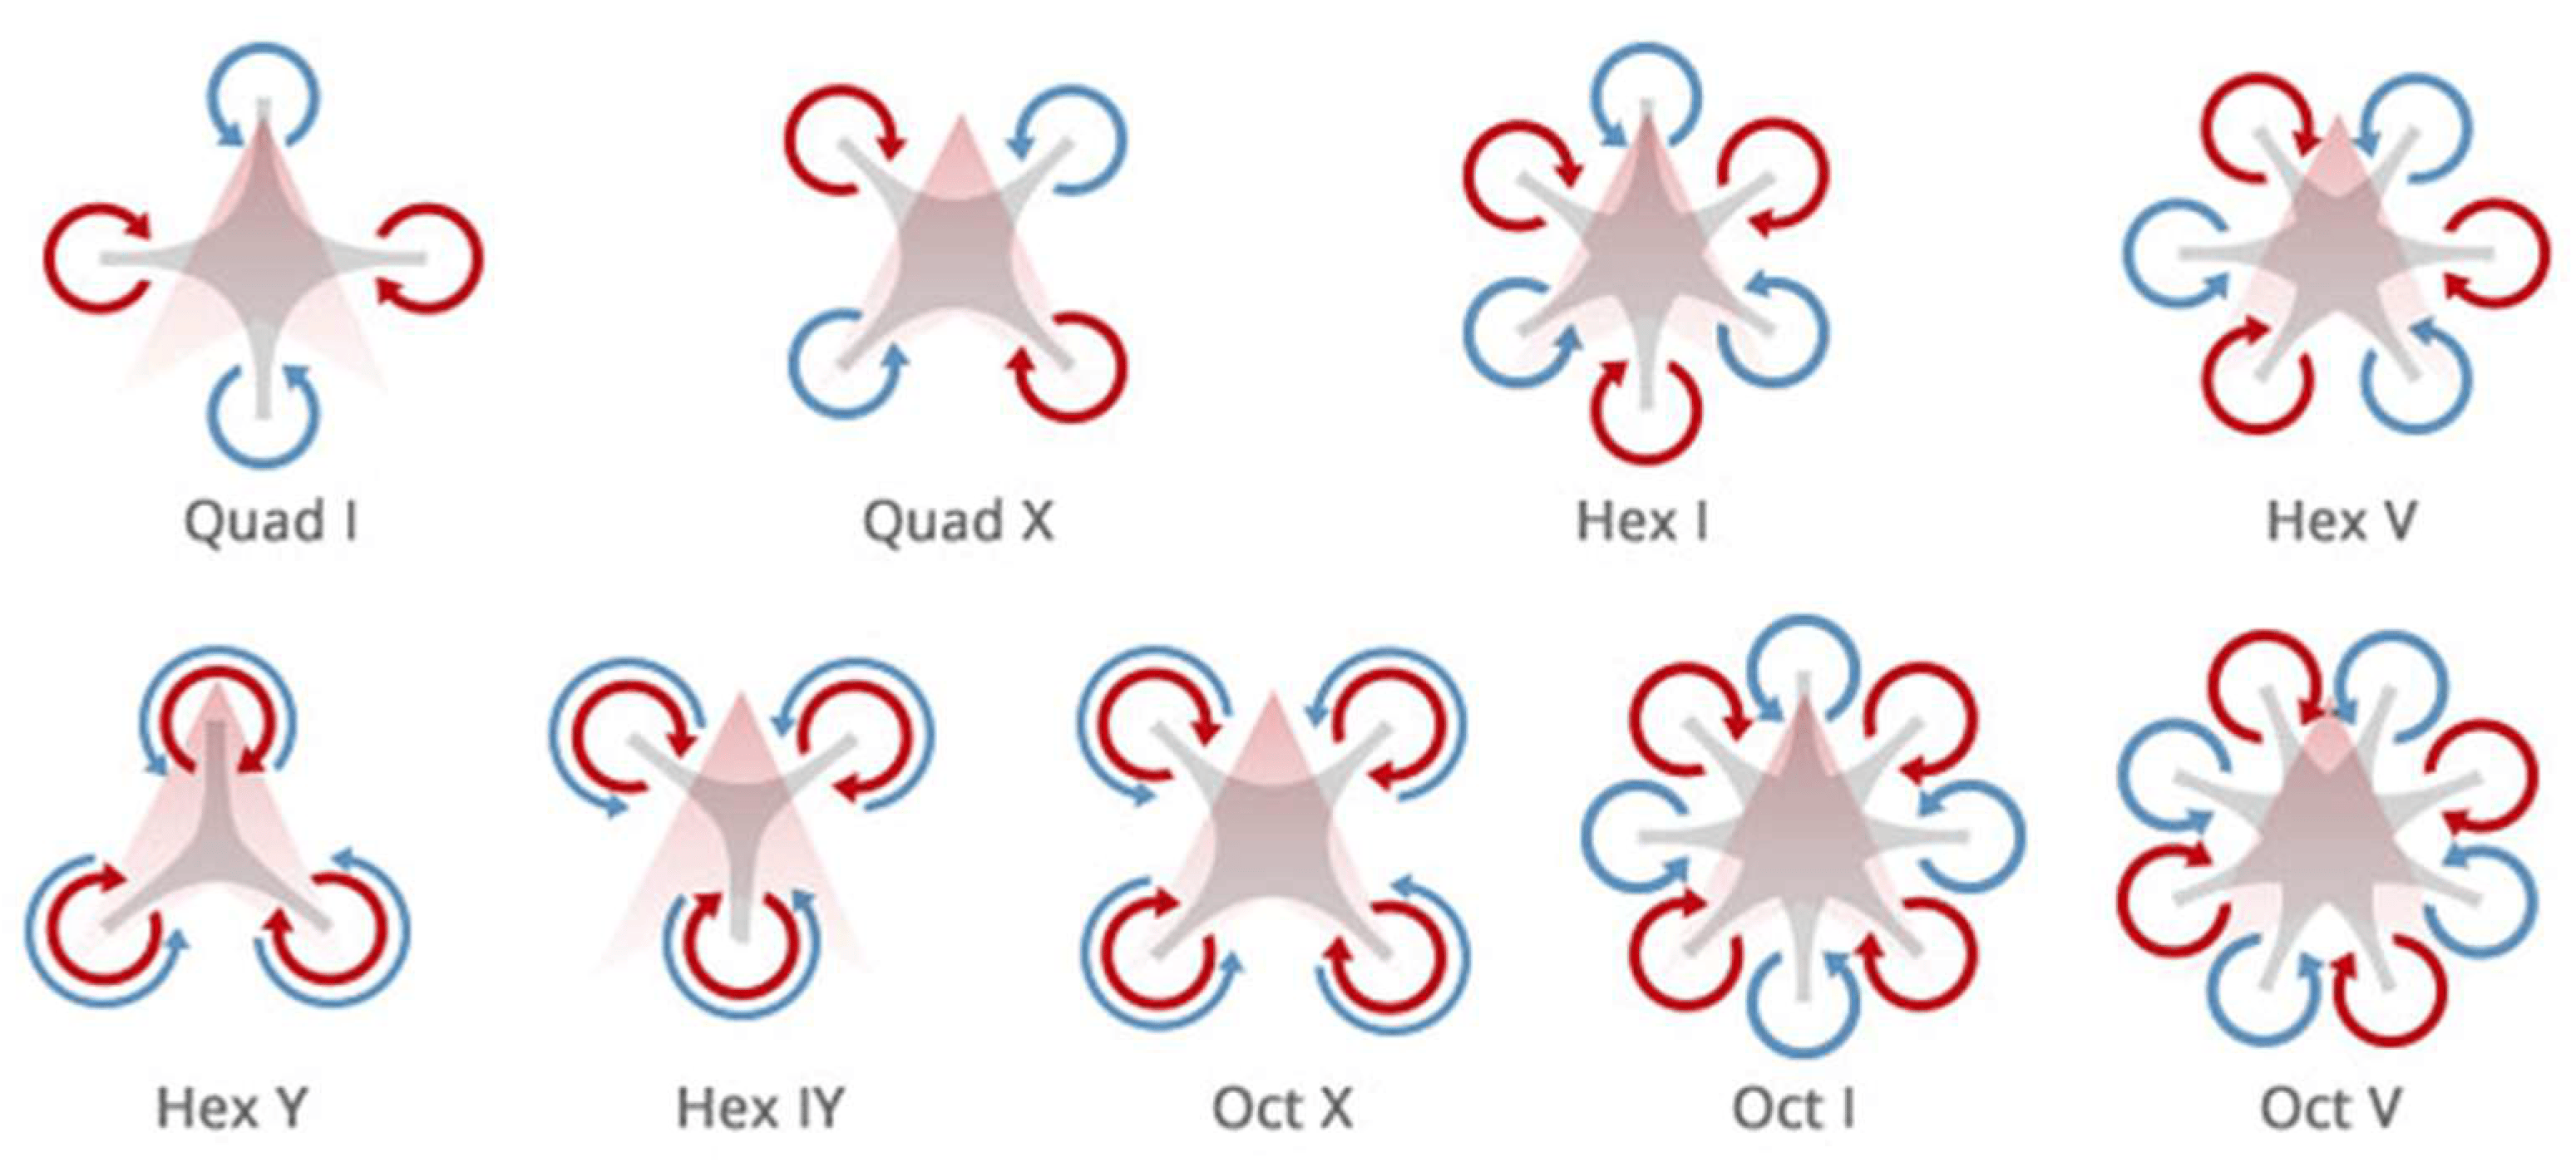
\includegraphics[width=0.75\textwidth]{gfx/drone_types}
    \caption[Classificazione multi-rotori.]{Classificazione multi-rotori in base al numero e alla configurazione dei rotori.}
    \label{fig:droneTypes}
\end{figure}

Nel seguito si prenderà come riferimento un quadrirotore con struttura a X dato che presenta un modello fisico-matematico semplificato e rende pertanto più semplice il progetto di schemi di controllo. Inoltre, questa disposizione dei rotori minimizza la variazione di posizione del baricentro e risulta pertanto più semplice tenere traccia della traiettoria del drone nello spazio.

% ------------------------------ MODELLAZIONE ------------------------------

\section{Modellazione Quadrirotore}
Un robot, nello specifico un quadrirotore, può essere considerato come un corpo rigido che trasla e ruota in uno spazio tridimensionale. Pertanto, è necessario costruire un modello matematico in grado di descrivere in modo compatto il suo spostamento.\\

Il modello fisico-matematico di un quadrirotore si può trovare con diversi formalismi, quali quello di Newton-Eulero e quello di Lagrange \cite{modelloQuad1} \cite{modelloQuad2} \cite{modelloQuad3}. Nel seguito si descrive il primo.\\

Nello specifico, si tratta di un sistema a sei gradi di libertà - 6 \ac{DoF} - quindi è descrivibile utilizzando dodici stati\footnote{Per ogni grado di libertà si considerano due stati: uno descrive la variabile considerata in un determinato istante di tempo $t$, l'altro ne descrive l'evoluzione nel tempo. Nel caso di un sistema tempo discreto è sufficiente calcolare la variabile nell'istante discreto successivo $t + T_C$, dove $T_C$ è il periodo di campionamento (Metodo Differenze Finite). Siccome $T_C$ è un tempo costante si può normalizzare il periodo di campionamento rendendolo unitario. Nel caso di un sistema tempo continuo si estende lo stesso ragionamento tramite l'operatore di derivata (Metodo Eulero). Se ad esempio la variabile considerata rappresenta una posizione, la sua evoluzione è una velocità.}: sei per la posizione, sei per l'assetto. Il sistema pertanto risulta sotto-attuato perché è caratterizzato da sei gradi di libertà, ma il suo movimento nello spazio può essere controllato soltanto da quattro attuatori (uno per ogni elica). In particolare, variando le velocità angolari delle eliche del velivolo è possibile effettuare tutti i movimenti.

\begin{figure}[H]
    \centering
    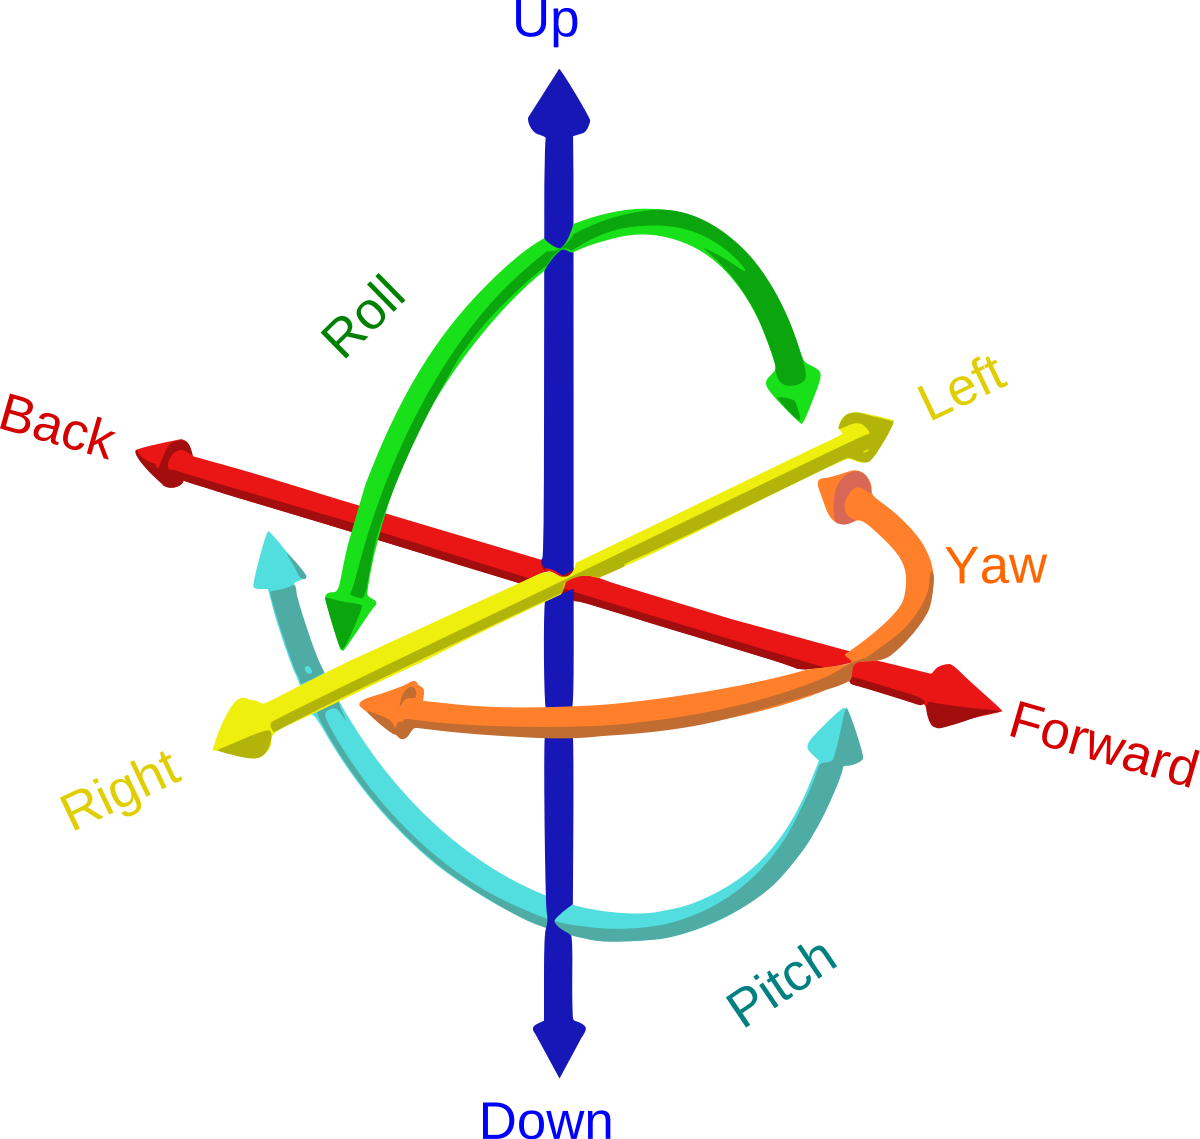
\includegraphics[width=0.3\textwidth]{gfx/6dof}
    \caption[Sei gradi di libertà (6 \acs{DoF}) di un corpo rigido in uno spazio tridimensionale.]{Sei gradi di libertà (6 \acs{DoF}) di un corpo rigido in uno spazio tridimensionale.}
\end{figure}

\subsection{Sistemi di Riferimento}

Prima di poter descrivere le equazioni che governano un velivolo, come il quadrirotore, è necessario definire le coordinate di riferimento in cui si intende farlo. Sono necessari due sistemi di riferimento per descrivere la posizione e l'assetto del drone nello spazio: un sistema \emph{mondo} (earth frame o $E$) inerziale, e un sistema \emph{drone} (body frame o $B$) solidale al velivolo in movimento, le cui dinamiche possono essere espresse rispetto alla terna fissa. La terna fissa (inerziale) è una terna dove si può considerare valida la prima legge di Newton.\\

Il sistema \emph{mondo} può essere definito secondo le coordinate \ac{LTP}, relative al piano tangente ad ogni punto della superficie terrestre. Esistono due convenzioni: il sistema \ac{ENU} è definito da una terna i cui versori sono orientati verso Est, Nord (piano tangente) e verso l'esterno della terra (Figura \ref{fig:fixedRef}), il sistema \ac{NED} è definito analogamente con Est e Nord scambiati e punta verso l'interno della terra.

\begin{figure}[H]
    \centering
    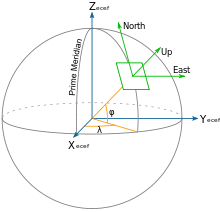
\includegraphics[width=0.29\textwidth]{gfx/ltp_enu}
    \caption[Sistema di riferimento \acs{ENU}.]{Sistema di riferimento \acs{ENU}, tangente alla superficie terrestre.}
    \label{fig:fixedRef}
\end{figure}

Il sistema \emph{drone} ha origine nel centro di massa del quadrirotore e in letteratura viene definito come \ac{ABC}. Questa terna mobile varia a seconda della configurazione dei rotori del quadrirotore, come mostra Figura \ref{fig:+andx}. Nel caso di un quadrirotore con disposizione a + si considerano gli assi x e y coincidenti con i due assi principali del quadrirotore. Nel caso in oggetto (disposizione a X), invece, gli assi x e y corrispondono alle bisettrici dei due assi principali del quadrirotore.

\begin{figure}[H]
    \centering
    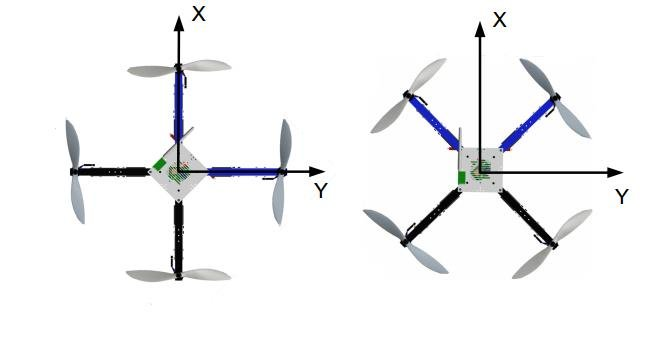
\includegraphics[width=0.53\textwidth]{gfx/+andx}
    \caption[\acs{ABC} di un QUAD I e di un QUAD X.]{\acs{ABC} di un QUAD I e di un QUAD X.}
    \label{fig:+andx}
\end{figure}

\begin{figure}[H]
    \centering
    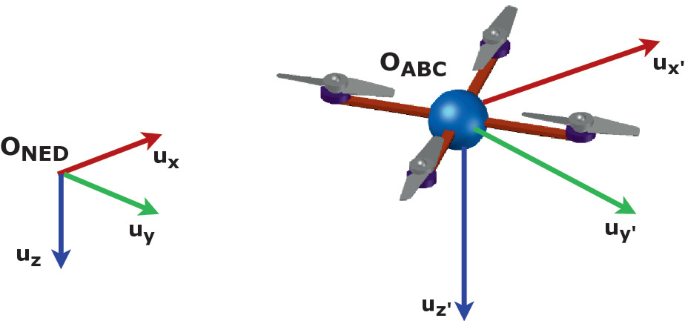
\includegraphics[width=0.7\textwidth]{gfx/abc_frame}
    \caption[Sistemi di riferimento \acs{NED} e \acs{ABC}.]{Sistemi di riferimento \acs{NED} e \acs{ABC}, utilizzati nella modellazione di un quadrirotore.}
    \label{fig:abc_frame}
\end{figure}

\subsection{Trasformazioni}

Dato che il drone trasla e ruota, è necessario stabilire per entrambi i moti un modo per poter passare dal sistema di riferimento \emph{mondo} al sistema di riferimento \emph{drone} e viceversa. 

\section*{Traslazioni}
Per le traslazioni è sufficiente utilizzare la somma vettoriale nello spazio a tre dimensioni di riferimento. Infatti, dato un generico punto $P$ rappresentato nel sistema di riferimento del velivolo $O_{ABC}$ dal vettore $v^P_{ABC}$, esiste un vettore di traslazione che permette di rappresentare lo stesso punto nel sistema di riferimento a terra. Nello specifico:
\[ v^p_{NED} = v^p_{ABC} + t_{NED} \]
dove $v^P_{NED}$ è il vettore che rappresenta il punto $P$ nel sistema di riferimento a terra e $t_{NED}$ è il vettore di traslazione. 

\section*{Rotazioni}
Le rotazioni possono essere descritte assumendo il corpo rigido fisso (in termini di posizione) nell'origine di un sistema di riferimento, con i tre versori del sistema che cambiano sotto l'effetto di rotazioni. Quindi, la rotazione è una relazione tra un sistema di riferimento fisso e lo stesso sistema (cioè con stessa origine) ruotato rispetto ai tre angoli di Eulero (cioè rispetto ai tre assi). La rotazione di un angolo intorno ad un asse può essere rappresentata da una matrice le cui colonne corrispondono ai versori del sistema ruotato. Considerando i tre possibili angoli di rotazione relativi ai tre assi del sistema di riferimento, si ottengono le seguenti tre matrici di rotazione ortonormali, cioè tali che $R^\top = R^{-1}$.

\begin{itemize}
	\item Rotazione intorno all'asse x:
	\begin{equation}
	R_x(\phi) = 
	\begin{bmatrix}
		1 & 0 & 0\\
		0 & \cos(\phi) & \sin(\phi)\\
		0 & -\sin(\phi) & \cos(\phi)
	\end{bmatrix}
	\end{equation}
	\item Rotazione intorno all'asse y:
	\begin{equation}
	R_y(\theta) = 
	\begin{bmatrix}
		\cos(\theta) & 0 & \sin(\theta)\\
		0 & 1 & 0\\
		-\sin(\theta) & 0 & \cos(\theta)
	\end{bmatrix}
	\end{equation}
	\item Rotazione introno all'asse z:
	\begin{equation}
	R_z(\psi) = 
	\begin{bmatrix}
		\cos(\psi) & \sin(\psi) & 0\\
		-\sin(\psi) & \cos(\psi) & 0\\
		0 & 0 & 1
	\end{bmatrix}
	\end{equation}
\end{itemize}

Quindi, dato un generico punto $P$ rappresentato nel sistema di riferimento traslato ma non ruotato $O_{xyz}$ dal vettore $v^P_{xyz}$, la trasformazione che consente di rappresentare lo stesso punto nel sistema di riferimento $O_{x'y'z'}$ ruotato intorno all'origine rispetto ad uno specifico asse (e.g. asse x) è la seguente:
\[ v^P_{x'y'z'} =  R_x(\bar{\phi})v^P_{xyz}\]
dove $v^P_{x'y'z'}$ è il vettore che rappresenta $P$ nel sistema ruotato intorno all'asse x di un angolo $\bar{\phi}$, come indicato nella matrice di rotazione.\\

A questo punto, si definisce la \ac{DCM} come il prodotto delle tre matrici di rotazione per passare da un sistema di riferimento all'altro. Per semplificare la notazione, le funzioni trigonometriche  $\sin (\cdot)$ e $\cos (\cdot)$ sono talvolta indicate come $s(\cdot)$ e $c(\cdot)$, rispettivamente.\\

Per passare dal sistema \emph{mondo} al sistema \emph{drone} si considera la seguente matrice di trasformazione:
\[
R_{EB}(\phi,\theta,\psi) = 
R_x(\phi)R_y(\theta)R_z(\psi) = 
\]
\begin{equation}
=
\begin{bmatrix}
c(\theta)c(\psi) & c(\theta)s(\psi) & -s(\theta)\\
s(\phi)s(\theta)c(\psi)-c(\phi)s(\psi) & s(\phi)s(\theta)c(\psi)+c(\phi)c(\psi) & s(\phi)c(\theta)\\
c(\phi)s(\theta)c(\psi)+s(\phi)s(\psi) & c(\phi)s(\theta)s(\psi)-s(\phi)c(\psi) & c(\phi)c(\theta)
\end{bmatrix}
\label{dcmEB}
\end{equation}

Per passare dal sistema \emph{drone} al sistema \emph{mondo}, invece, si considera la seguente matrice di trasformazione:
\[
R_{BE}(\phi,\theta,\psi) = 
R_z(\psi)R_y(\theta)R_x(\phi) = 
\]
\begin{equation}
=
\begin{bmatrix}
c(\theta)c(\psi) & -c(\phi)s(\psi)+s(\phi)s(\theta)c(\psi) & s(\phi)s(\psi)+c(\phi)s(\theta)c(\psi)\\
s(\psi)c(\theta) & c(\theta)c(\psi)+s(\phi)s(\theta)s(\psi) & s(\theta)c(\phi)s(\psi)-s(\phi)c(\psi)\\
-s(\theta) & c(\theta)s(\phi) & c(\theta)c(\phi)
\end{bmatrix}
\label{dcmBE}
\end{equation}

\subsection{Modello Non Lineare}

I sei stati di posizione descrivono la posizione del drone e la sua evoluzione nel tempo, cioè come il velivolo trasla rispetto al sistema a terra. I sei stati di assetto descrivono l'assetto del drone e la sua evoluzione nel tempo, cioè come il velivolo ruota introno all'origine del sistema di riferimento traslato. A tal proposito, in aeronautica si utilizzano gli angoli di Eulero: rollio (roll o $\phi$), beccheggio (pitch o $\theta$) e imbardata (yaw o $\psi$); che indicano rispettivamente una rotazione intorno agli assi Y, X e Z, come mostra Figura  \ref{fig:quadModel}.

\begin{figure}[H]
    \centering
    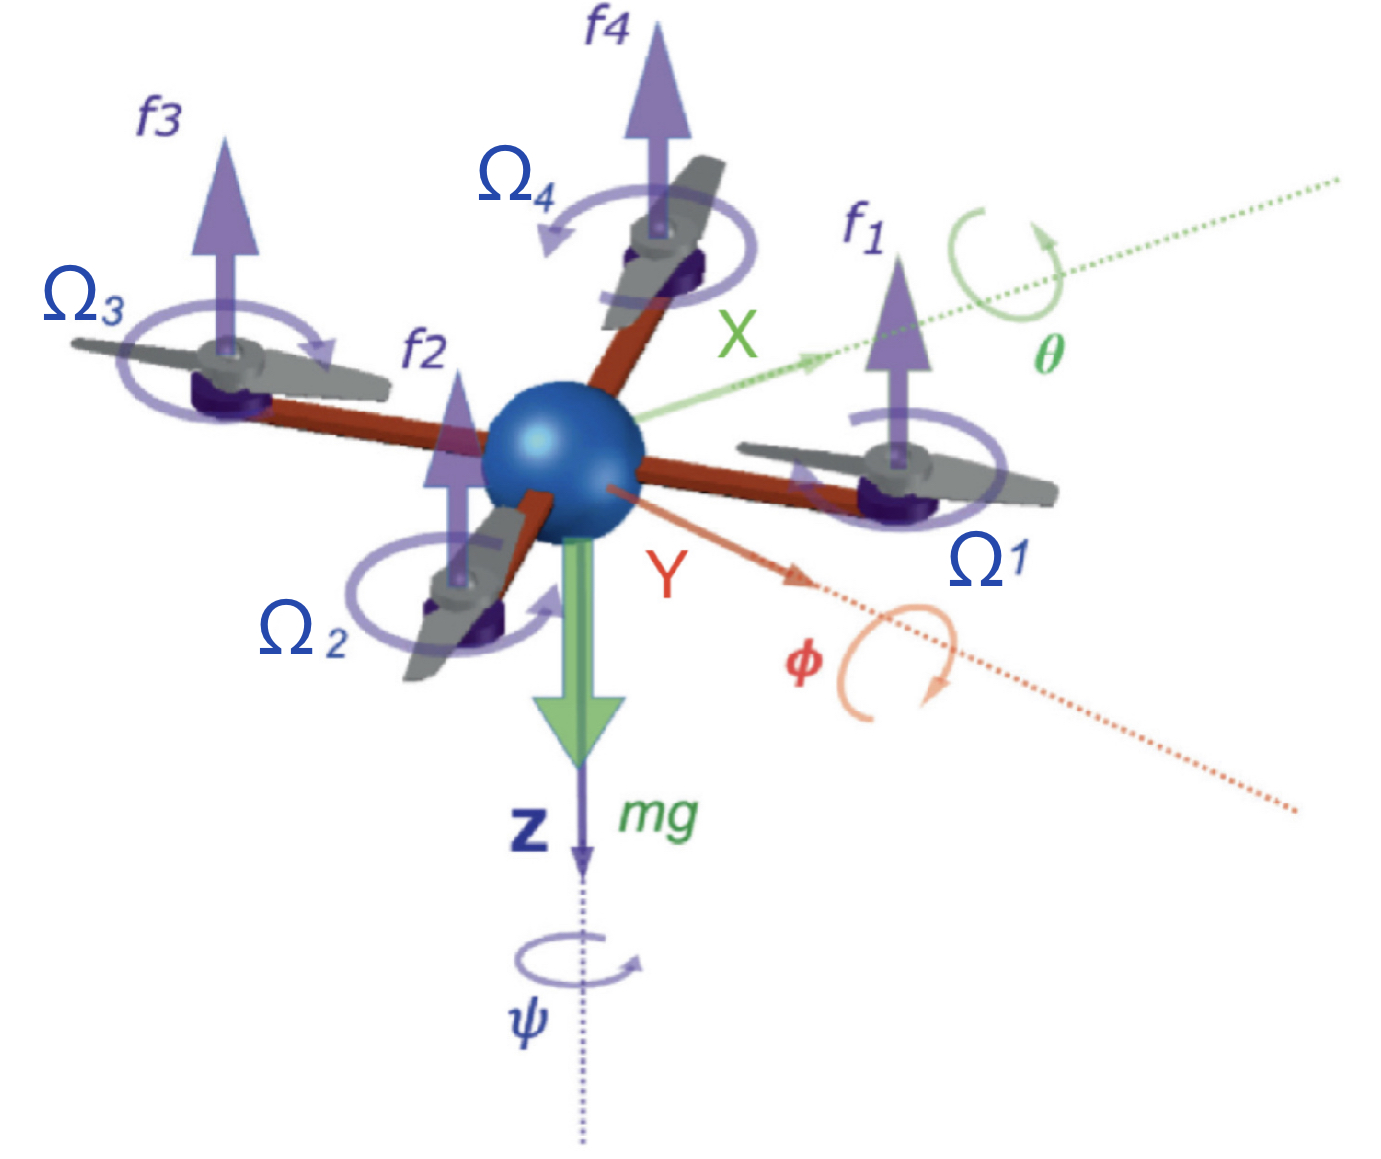
\includegraphics[width=0.5\textwidth]{gfx/quad_model}
    \caption[Modello fisico del quadrirotore, con velocità angolari dei rotori.]{Modello fisico del quadrirotore, dove $\Omega_i$ e $f_i $ ($i = 1,2,3,4$) sono rispettivamente le velocità angolari dei rotori e le relative forze di spinta generate.}
    \label{fig:quadModel}
\end{figure}

Si definiscono quattro vettori tridimensionali per rappresentare i dodici stati del modello. I primi due vettori sono definiti rispetto al sistema di riferimento \emph{mondo} ($E$) e rappresentano rispettivamente il vettore di posizione che identifica la posizione del drone nello spazio (\ref{statePos}) e il vettore di assetto che descrive (secondo gli angoli di Eulero) come il drone è ruotato intorno agli assi coordinati (\ref{stateEul}).

\begin{equation}
\Gamma_E = \begin{bmatrix}
x & y & z 
\end{bmatrix}^\top
\label{statePos}
\end{equation}

\begin{equation}
\Theta_E = \begin{bmatrix}
\phi & \theta & \psi
\end{bmatrix}^\top
\label{stateEul}
\end{equation}

I restanti vettori sono definiti rispetto al sistema di riferimento \emph{drone} ($B$) e rappresentano rispettivamente la velocità lineare (\ref{stateVelLin}) e la velocità angolare (\ref{stateVelAng}) del quadrirotore.

\begin{equation}
V_B = \begin{bmatrix}
u & v & w
\end{bmatrix}^\top
\label{stateVelLin}
\end{equation}

\begin{equation}
\omega_B = \begin{bmatrix}
p & q & r 
\end{bmatrix}^\top
\label{stateVelAng}
\end{equation}

Il moto di traslazione del velivolo è definito dall'equazione \ref{eqSist1} seguente, che mette in relazione $\Gamma_E$ e $V_B$ tramite la matrice $R_{BE}$ (\acs{DCM} definita dalla \ref{dcmBE}). 

\begin{equation}
	\dt{\Gamma_E} = R_{BE}V_B
	\label{eqSist1}
\end{equation}

Il moto di rotazione, invece, mette in relazione $\Theta_E$ e $\omega_B$. In questo caso entra in gioco una nuova matrice $J$ che consente di trasformare le variazioni degli angoli di Eulero intorno ai rispettivi assi ($\dt{\phi}, \dt{\theta}, \dt{\psi}$) nel vettore di velocità angolare del quadrirotore $\omega_B$, come mostra l'equazione \ref{jacobian}.

\begin{equation}
	J\dt{\Theta_E} = \omega_B
	\label{jacobian}
\end{equation}

Considerando la matrice inversa (\ref{invJacobian}) si ottiene l'equazione del moto di rotazione cercata (\ref{eqSist2}).

\begin{equation}
	\dt{\Theta_E} = J^{-1}\omega_B
	\label{eqSist2}
\end{equation}

\begin{equation}
J^{-1}
=
\begin{bmatrix}
1 & \sin(\phi)\tan(\theta) & \cos(\phi)\tan(\theta)\\
0 & \cos(\phi) & -\sin(\phi)\\
0 & \frac{\sin(\phi)}{\sin(\theta)} & \frac{\cos(\phi)}{\cos(\theta)}
\end{bmatrix}
\label{invJacobian}
\end{equation}\\

Prima di poter formulare il modello matematico del quadrirotore è necessario fare un'ipotesi semplificativa. Ogni sistema rotante, infatti, risente del cosiddetto effetto giroscopico, cioè un fenomeno che tende a mantenere il sistema sul suo asse di rotazione. Risulta quindi più difficile cambiare l’assetto, ma siccome l’effetto è tanto più forte quanto più la velocità di rotazione è grande, e in questo caso non ci sono grandi velocità, l’effetto è trascurabile. Si può dimostrare che trascurandolo, il modello può essere quindi scritto con il seguente sistema di equazioni nel sistema di riferimento \emph{drone}.

\begin{equation}
	\begin{cases}
	\Dot{u} = (vr - wq) + g\sin((\theta) \\
	\Dot{v} = (wp - ur) - g\cos(\theta)\sin(\phi) \\
	\Dot{w} = (uq - vp) - g\cos(\theta)\sin(\phi) + \frac{U_1}{m} \\
	\Dot{p} = \frac{I_{YY} - I_{ZZ}}{I_{XX}}qr + \frac{U_2}{I_{XX}} \\
	\Dot{q} = \frac{I_{ZZ} - I_{XX}}{I_{YY}}pr + \frac{U_3}{I_{YY}} \\
	\Dot{r} = \frac{I_{XX} - I_{YY}}{I_{ZZ}}pq + \frac{U_4}{I_{ZZ}}
	\end{cases}
	\label{modelloQuadrirotoreDrone}
\end{equation}

Dove i termini $U_i$ ($i = 1,2,3,4$) sono i termini di controllo del quadrirotore e sono infatti definiti in funzione delle velocità angolari dei rotori $\Omega_i$ ($i = 1,2,3,4$), come mostra la \ref{defControls}.

\begin{equation}
	\begin{cases}
	U_1 = b({\Omega_1}^2 + {\Omega_2}^2 + {\Omega_3}^2 + {\Omega_4}^2) \\
	U_2 = lb(- {\Omega_2}^2 + {\Omega_4}^2) \\
	U_3 = lb(- {\Omega_1}^2 + {\Omega_3}^2) \\
	U_4 = d(- {\Omega_1}^2 + {\Omega_2}^2 - {\Omega_3}^2 + {\Omega_4}^2)
	\end{cases}
	\label{defControls}
\end{equation}

Inoltre, nel modello (\ref{modelloQuadrirotoreDrone}) sono presenti i termini $I_{XX}, I_{YY}, I_{ZZ}$, cioè gli elementi diagonali della matrice di inerzia $I$, indicata nella \ref{matInerzia}. Quest'ultima risulta diagonale perché per ipotesi l'origine del sistema di riferimento del drone è nel suo centro di massa e gli assi corrispondono agli assi principali di inerzia.
 
\begin{equation}
I =
\begin{bmatrix}
I_{XX} & 0 & 0\\
0 & I_{YY} & 0\\
0 & 0 & I_{ZZ}
\end{bmatrix}
\label{matInerzia}
\end{equation}

Infine, vale la pena spiegare il significato dei coefficienti $b$ e $d$, che legano le velocità angolari dei rotori ai termini di controllo.\\

Il termine $b$ è il cosiddetto coefficiente di thrust. È un coefficiente che lega la spinta alla velocità angolare secondo la seguente equazione.

\begin{equation}
	b = \frac{T}{\Omega^2}
	\label{thrustCoeff}
\end{equation}

Dove $\Omega$ è la velocità di un generico rotore e $T$ è la spinta che genera verso l'alto. Si misura in $[N s^2]$ ed è considerato costante e uguale per tutti i rotori. La spinta verso l'altro è pertanto descritta dal termine di controllo $U_1$ nella \ref{defControls}.\\

Il termine $d$ è il cosiddetto coefficiente di drag. Quando le pale di un rotore girano in un certo verso, nasce una forza dovuta alla resistenza del vento nel senso opposto che genera un momento. Nella dinamica del quadrirotore, il coefficiente $d$ incide sull'angolo di imbardata, legato alla variazione dei momenti. Anche questo coefficiente è considerato costante e uguale per tutti i rotori, si misura in $[N m s^2]$ ed è definito come segue:

\begin{equation}
	d = \frac{Q}{\Omega^2}
\end{equation}

dove $Q$ è il momento della forza di trascinamento. Nella \ref{defControls} il termine $U_4$ tiene conto di questo contributo.\\

Poi, i termini $U_2$ e $U_3$ sono legati rispettivamente agli angoli di roll e pitch. Nello specifico, $U_2$ è legato alla differenza delle spinte date dai rotori di indice due e quattro, cioè (dalla \ref{thrustCoeff}) ai prodotti $b{\Omega_2}^2$ e $b{\Omega_4}^2$, poi moltiplicata per il braccio $l$. Analogo è il discorso per $U_3$, ma chiaramente interessa i rotori di indice uno e tre.\\

Si può anche scrivere il modello dinamico riferito al sistema \emph{mondo} tramite il seguente sistema di equazioni \ref{modelloQuadrirotoreMondo}.

\begin{equation}
	\begin{cases}
	\Ddot{X} = (sin(\psi)sin(\phi) + cos(\psi)sin(\theta)cos(\phi))\frac{U_1}{m} \\
	\Ddot{Y} = (-cos(\psi)sin(\phi) + sin(\psi)sin(\theta)cos(\phi))\frac{U_1}{m} \\
	\Ddot{Z} = -g + (cos(\theta)cos(\phi))\frac{U_1}{m} \\
	\Dot{\phi} = p + sin(\phi)tan(\theta)q + cos(\phi)tan(\theta)r \\
	\Dot{\theta} = cos(\phi)q + cos(\theta)sin(\phi)r \\
	\Dot{\psi} = -sin(\phi)q + cos(\theta)cos(\phi)r
	\end{cases}
	\label{modelloQuadrirotoreMondo}
\end{equation}

Si nota facilmente che il modello dinamico ottenuto (definito dalla \ref{modelloQuadrirotoreDrone} nel sistema solidale al drone e dalla \ref{modelloQuadrirotoreMondo} nel sistema solidale alla terra) è di tipo non lineare.

% ------------------------------ QUATERNIONI ------------------------------

\section{Angoli di Eulero e Quaternioni}
Come spiegato nel paragrafo precedente, ogni rotazione di un corpo rigido può essere descritta mediante i tre angli di Eulero, che specificano una sequenza di tre rotazioni successive intorno agli assi coordinati. Da un lato questa rappresentazione risulta facile da comprendere e, dal punto di vista dell'implementazione, necessita semplicemente di tre numeri reali floating point. Dall'altro soffre il problema del gimbal lock (o blocco cardanico).\\

\subsection{Gimbal Lock}
Si tratta di un fenomeno problematico dei giroscopi causato dall'allineamento di due assi rotanti verso la stessa direzione. Il blocco causa la perdita del grado di libertà corrispondente all'asse bloccato.\\

Nello specifico, il problema si verifica quando il valore di alcuni angoli raggiunge valori critici. Infatti, se ad esempio il valore dell'angolo di pitch ($\theta$) dovesse raggiungere i 90 gradi, il sensore a bordo del velivolo non sarebbe in grado di distinguere tra roll ($\phi$) e yaw ($\psi$). Osservando la Figura \ref{fig:gimbal_lock} si nota come l'orientazione relativa al caso B possa essere frutto di due rotazioni differenti: un beccheggio seguito da un rollio oppure un'imbardata seguita da un beccheggio.

\begin{figure}[H]
    \centering
    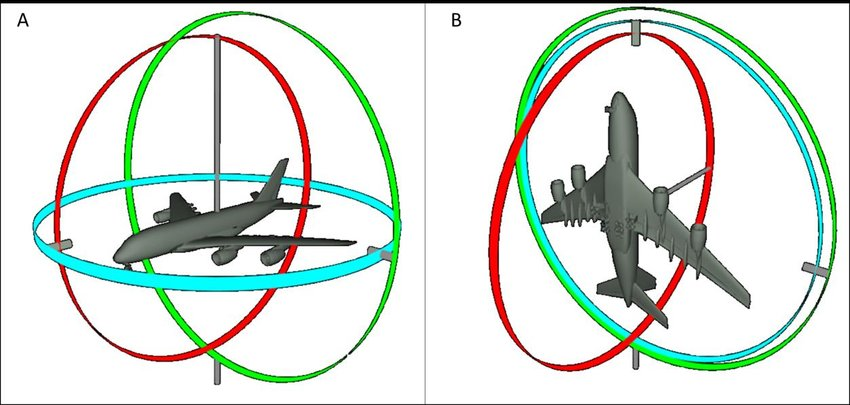
\includegraphics[width=0.7\textwidth]{gfx/gimbal_lock}
    \caption[Problema del blocco cardanico.]{Problema del blocco cardanico. Caso A: non si verifica il blocco cardanico. Caso B: rollio (roll) e imbardata (yaw) sono bloccati e risultano indistinguibili, quindi si perde un grado di libertà (blocco cardanico).}
    \label{fig:gimbal_lock}
\end{figure}

Questa problematica si riscontra facilmente anche nel modello matematico. Infatti, osservando la matrice $T$ che descrive il moto rotazionale del quadrirotore, si nota come per $\theta = \pm 90 \deg$ questa risulta singolare (determinante nullo).\\

Esistono due metodi differenti per risolvere questo problema. Il primo prevede semplicemente di utilizzare gli angoli di Eulero ad una condizione: gli angoli misurati dai sensori devono mantenersi piccoli. Il secondo, molto utilizzato, consiste nell'utilizzo dei quaternioni.

\subsection{Quaternioni}
Introdotto da William Rowan Hamilton nel 1843 come estensione dei numeri complessi, un quaternione è un elemento scrivibile come:
\[ a + bi + cj + dk \]
dove $a, b, c, d$ sono numeri reali e $i, j, k$ si comportano in modo simile all'unità immaginaria dei numeri complessi. Si può dire che la prima coordinata $a$ costituisce la parte scalare o reale del quaternione, mentre le rimanenti tre coordinate $b, c, d$ ne costituiscono la parte vettoriale o immaginaria.\\

Pertanto, un quaternione è identificato da quattro numeri reali e può essere scritto come un vettore di $\mathbb{R}^4$ come segue.
\[
q = \begin{bmatrix}
q_0 & q_1 & q_2 & q_3
\end{bmatrix}^\top
\]
con $q_0, q_1, q_2, q_3 \in \mathbb{R}$.\\

Un quaternione unitario è un quaternione di norma unitaria.
\[ || q || = q_0^2 + q_1^2 + q_2^2 + q_3^2 = 1 \]

La totalità dei quaternioni unitari forma una ipersfera quadrimensionale in $\mathbb{R}^4$.
\[ S^3 = \{ (q_0, q_1, q_2, q_3) \in \mathbb{R}^4 | q_0^2 + q_1^2 + q_2^2 + q_3^2 = 1\} \]

 Questi particolari quaternioni possono essere utilizzati per descrivere l'assetto del quadrirotore nel sistema di riferimento \acs{ABC} rispetto al sistema di riferimento inerziale fisso.

\begin{figure}[H]
    \centering
    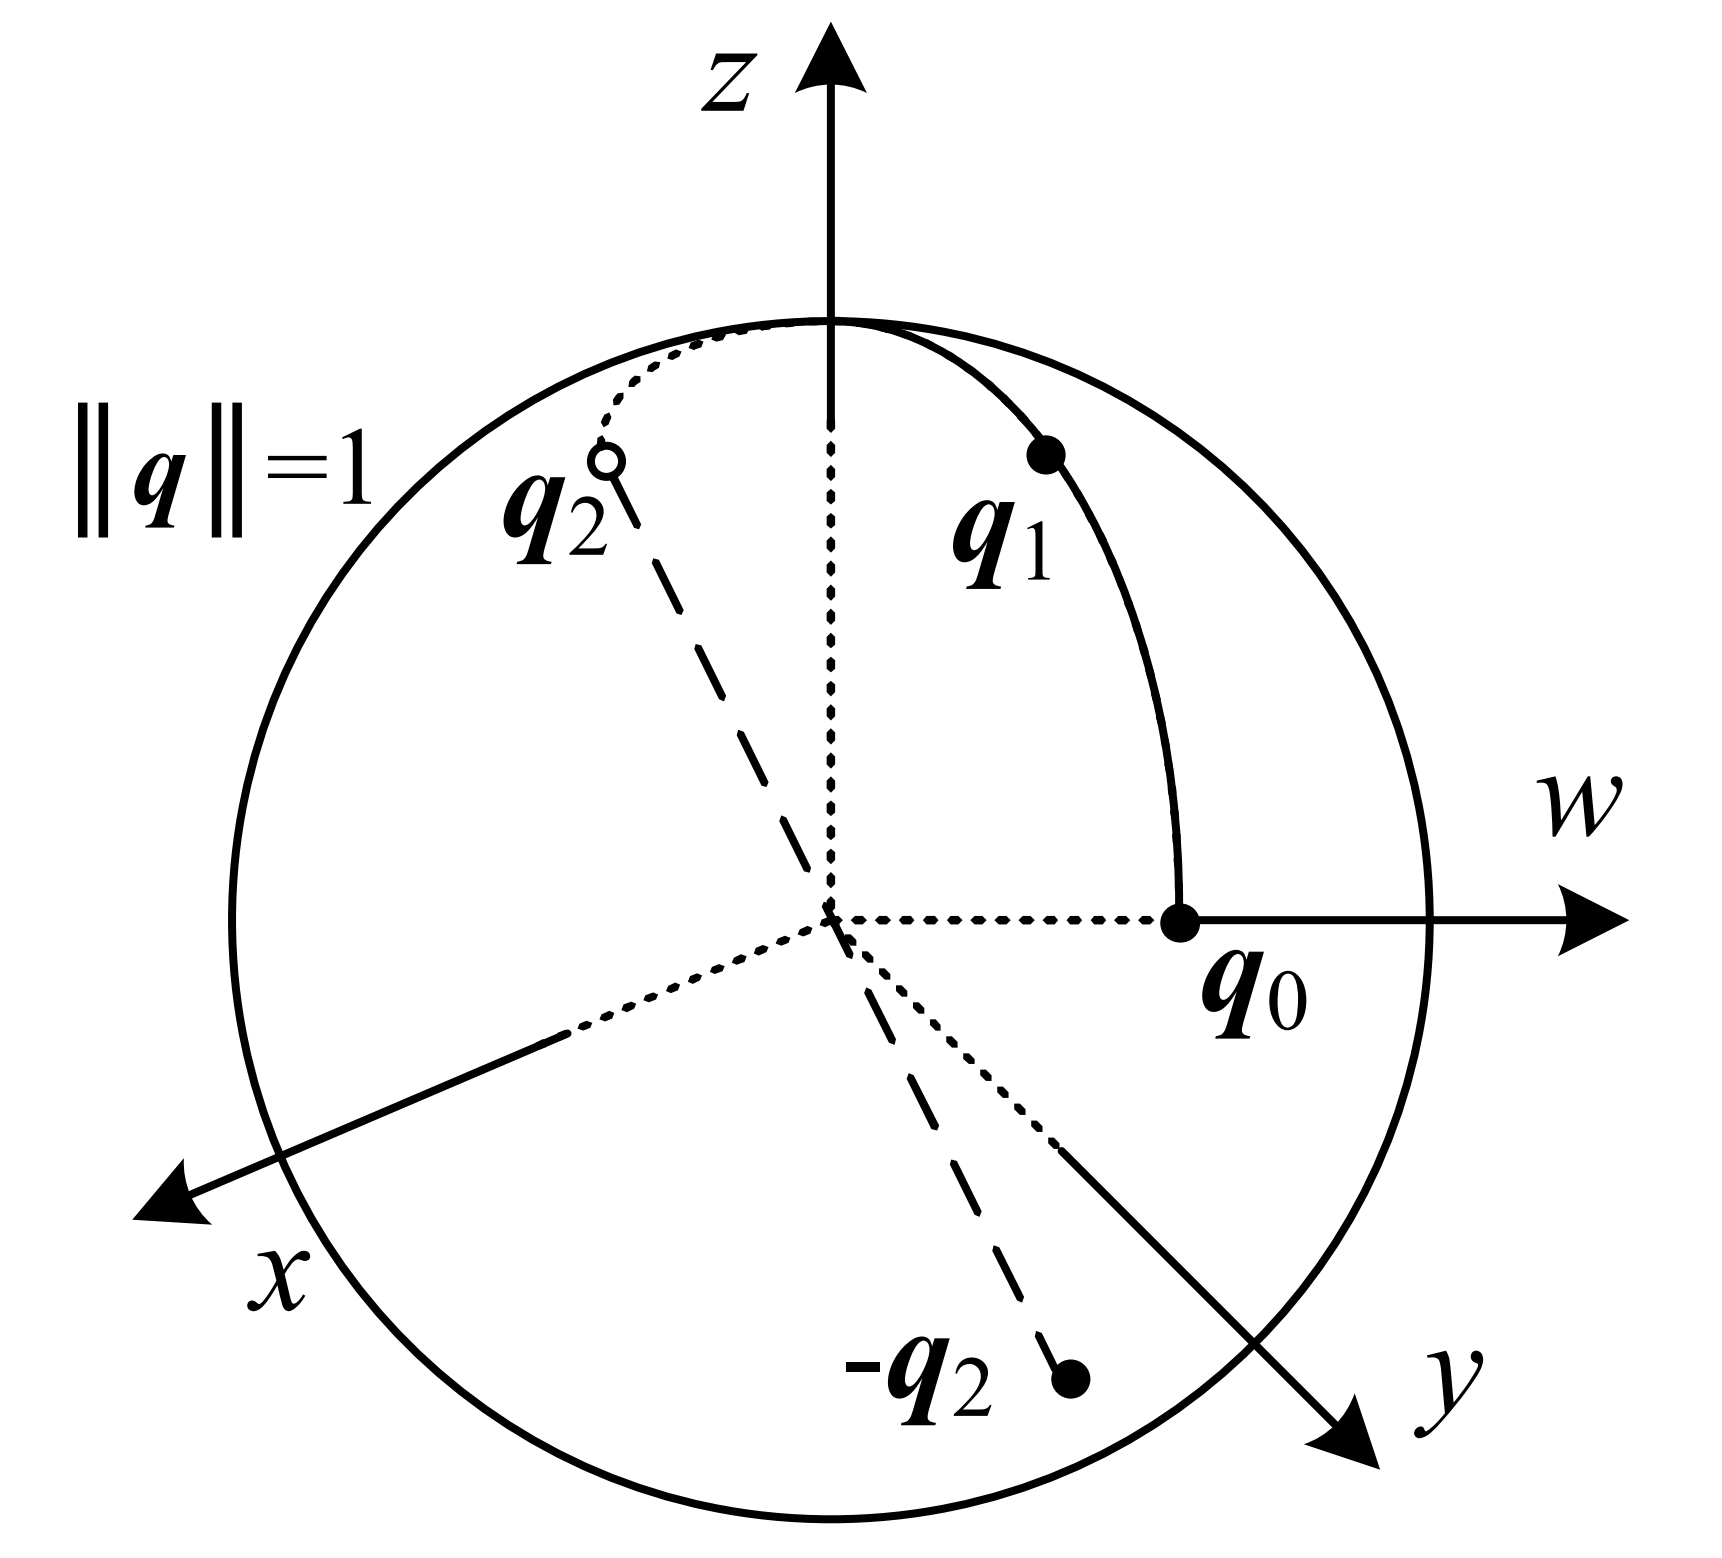
\includegraphics[width=0.5\textwidth]{gfx/quaternion}
    \caption[Rappresentazione grafica di una rotazione tramite un quaternione unitario.]{Rappresentazione grafica di una rotazione tramite un quaternione unitario.}
    \label{fig:quat}
\end{figure}

Somma e prodotto di due quaternioni sono definiti tenendo conto delle relazioni fondamentali\footnote{William Rowan Hamilton scrisse per la prima volta questa formula il 16 Ottobre 1843 camminando lungo il Broom Bridge, che attraversa il Royal Canal, a Cabra, Dublino, Irlanda. Tale evento è ad oggi commemorato da una targa collocata sul ponte che recita: "Mentre qui passeggiava, il 16 ottobre 1843 Sir William Rowan Hamilton, in un lampo d'ispirazione scoprì la formula fondamentale per la moltiplicazione dei quaternioni (\ref{hamiltonQuat}) e la incise su una pietra di questo ponte."}:
\begin{equation}
	 i^2 = j^2 = k^2 = ijk = -1
	 \label{hamiltonQuat}
\end{equation}\\

Le relazioni che legano gli angoli di Eulero ($\phi, \theta, \psi$) al quaternione unitario ($q$) corrispondente sono mostrate nelle equazioni \ref{quatEul} e \ref{eulQuat}.

\begin{equation}
	\begin{cases}
		q_0 = c(\frac{\phi}{2})c(\frac{\theta}{2})c(\frac{\psi}{2}) + s(\frac{\phi}{2})s(\frac{\theta}{2})s(\frac{\psi}{2}) \\
		q_1 = s(\frac{\phi}{2})c(\frac{\theta}{2})c(\frac{\psi}{2}) - c(\frac{\phi}{2})s(\frac{\theta}{2})s(\frac{\psi}{2}) \\
		q_2 = c(\frac{\phi}{2})s(\frac{\theta}{2})c(\frac{\psi}{2}) + s(\frac{\phi}{2})c(\frac{\theta}{2})s(\frac{\psi}{2}) \\
		q_3 = c(\frac{\phi}{2})c(\frac{\theta}{2})s(\frac{\psi}{2}) - s(\frac{\phi}{2})s(\frac{\theta}{2})c(\frac{\psi}{2})
	\end{cases}
	\label{quatEul}
\end{equation}

\begin{equation}
	\begin{cases}
		\phi = \tan^{-1} \left[\frac{2(q_2q_3 + q_0q_1)}{q_0^2 - q_1^2 - q_2^2 + q_3^2}\right] \\
		\theta = \sin^{-1} \left[-2(q_1q_3 + q_0q_2)\right] \\
		\psi = \tan^{-1} \left[\frac{2(q_1q_2 + q_0q_3)}{q_0^2 + q_1^2 - q_2^2 - q_3^2}\right]
	\end{cases}
	\label{eulQuat}
\end{equation}\\

Come detto, questa soluzione è ampiamente utilizzata in ambito informatico e robotico. Infatti, molti linguaggi di programmazione e molte librerie forniscono direttamente operazioni di conversione tra angoli di Eulero e quaternioni unitari, come si vedrà nel seguito.

% ------------------------------ CONTROLLO ------------------------------

\section{Controllo}
Un quadrirotore a X presenta quattro rotori posizionati come in Figura \ref{fig:quadRotors}. Essendo i motori e le eliche sullo stesso piano, è necessario equilibrare il moto del drone impiegando due motori che ruotano in senso orario e due che ruotano in senso antiorario. Nello specifico, i rotori M1 e M4 ruotano in senso orario (clockwise o CW), mentre i rotori M2 e M3 ruotano in senso antiorario (counterclockwise o CCW). Questa contrapposizione permette di annullare l'energia rotatoria dei motori e quindi eventuali coppie di reazione.

\begin{figure}[H]
    \centering
    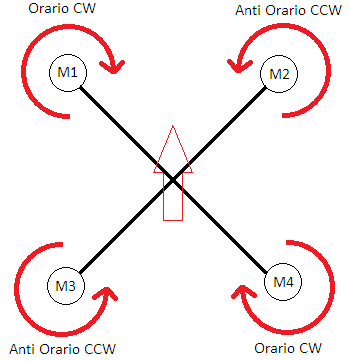
\includegraphics[width=0.3\textwidth]{gfx/rotori_quadrotor}
    \caption[Disposizione e funzionamento dei rotori di un quadrirotore con eliche disposte a X.]{Disposizione e funzionamento dei rotori di un quadrirotore con eliche disposte a X.}
    \label{fig:quadRotors}
\end{figure}

\subsection{Manovre di Spinta, Rollio, Beccheggio e Imbardata}

Nel seguito si descrive il funzionamento delle quattro principali manovre di controllo del quadrirotore. Tre di queste manovre sono dovute al cambiamento dell'assetto del drone nel tempo, cioè alle variazioni degli angoli di Eulero (rollio, beccheggio e imbardata). È possibile alterare questi angoli modificando le velocità dei quattro rotori in modo specifico. La quarta e ultima manovra di controllo, invece, riguarda la spinta del quadrirotore verso l'alto, mantenendone fisso l'assetto.

\section*{Manovra di Spinta}
Quando il vettore di spinta (thrust) è allineato alla verticale (direzione ortogonale al piano individuato dal quadrirotore) e ha modulo maggiore della forza peso del drone ($F_p = mg$ dove $m$ è la massa del drone e $g$ è l'accelerazione gravitazionale), si verifica una traslazione verticale lungo l'asse Z. Come specifica la relazione \ref{thrustCoeff}, la spinta generata è legata al quadrato delle velocità angolari dei rotori. In condizioni di equilibrio statico (hovering) ciascun rotore genera una spinta pari ad un quarto della forza peso del drone. Per aumentare il modulo della spinta verso l'alto (asse Z positivo) si aumentano le velocità di tutti i rotori di una stessa quantità, in modo da non creare differenze che possano modificare l'assetto del drone. In Figura \ref{fig:thrust_quad} è mostrato il concetto.

\begin{figure}[H]
    \centering
    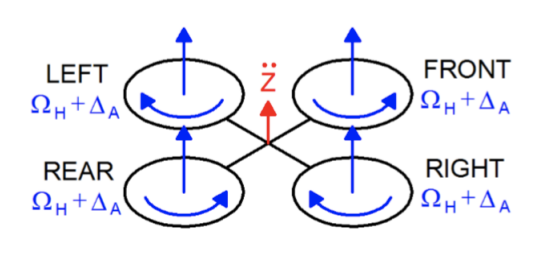
\includegraphics[width=0.5\textwidth]{gfx/thrust_quad}
    \caption[Manovra di spinta di un quadrirotore.]{Manovra di spinta: la velocità di tutti i rotori aumenta di una quantità costante.}
    \label{fig:thrust_quad}
\end{figure}

\pagebreak

\section*{Manovra di Rollio}
Il rollio contribuisce allo spostamento del drone lungo l'asse Y (destra e sinistra). Si ottiene lasciando invariate le velocità dei motori anteriore (FRONT) e posteriore (REAR), e cambiando di una certa quantità le velocità dei motori di destra (RIGHT) e sinistra (LEFT); come mostrato in Figura \ref{fig:roll_quad}.

\begin{figure}[H]
    \centering
    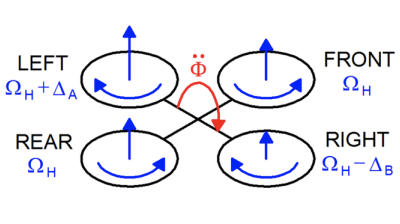
\includegraphics[width=0.39\textwidth]{gfx/roll_quad}
    \caption[Manovra di rollio di un quadrirotore.]{Manovra di rollio: cambia la velocità dei rotori di destra (RIGHT) e sinistra (LEFT).}
    \label{fig:roll_quad}
\end{figure}

\section*{Manovra di Beccheggio}
Il beccheggio contribuisce allo spostamento del drone lungo l'asse X (avanti e indietro). Si ottiene, analogamente al rollio, lasciando invariate le velocità dei motori di destra (RIGHT) e sinistra (LEFT), e cambiando di una certa quantità le velocità dei motori anteriore (FRONT) e posteriore (REAR); come mostrato in Figura \ref{fig:pitch_quad}.

\begin{figure}[H]
    \centering
    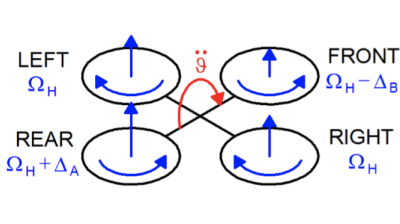
\includegraphics[width=0.39\textwidth]{gfx/pitch_quad}
    \caption[Manovra di beccheggio di un quadrirotore.]{Manovra di beccheggio: cambia la velocità dei rotori anteriore (FRONT) e posteriore (REAR).}
    \label{fig:pitch_quad}
\end{figure}

\pagebreak

\section*{Manovra di Imbardata}
L'imbardata è il movimento più complesso. L’idea fondamentale è cambiare il momento rispetto all’asse z, immaginato uscente dal piano dei rotori, e mantenere costante la spinta verso l’alto. Per ottenere questo, si aumenta la velocità dei rotori di due motori opposti, e si diminuisce la velocità dei due restanti rotori. In questo modo si avranno, per esempio, due rotori che girano velocemente in senso orario, e due che girano più lentamente in senso antiorario. Nel complesso ci sarà dunque un momento che fa girare il drone intorno all’asse z. Se le velocità sono opportunamente scelte, non ci sarà un cambiamento della spinta verso l’alto. La Figura \ref{fig:yaw_quad} riassume quanto detto.

\begin{figure}[H]
    \centering
    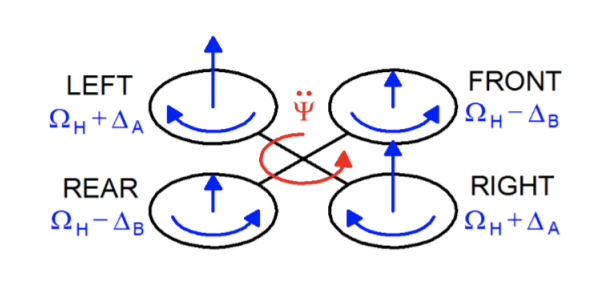
\includegraphics[width=0.47\textwidth]{gfx/yaw_quad}
    \caption[Manovra di imbardata di un quadrirotorre.]{Manovra di imbardata.}
    \label{fig:yaw_quad}
\end{figure}

\subsection{Controllo Stabilizzato e Acrobatico}
Esistono due modalità di volo e quindi di controllo di un quadrirotore. La modalità stabilizzata, anche nota come self-level, e la modalità acrobatica, anche nota come rates e utilizzata per droni da gara.\\

Nel primo caso si controlla il drone agendo sugli angoli di Eulero, come esposto nel paragrafo precedente. Nel secondo caso, invece, il segnale di controllo inviato al drone non contiene gli angoli di Eulero, ma le velocità angolari. Questo significa che, controllando il drone ad esempio con un radiocomando e lasciando andare le levette di roll e pitch verso il centro (cioè portandole a zero), nel primo caso il velivolo ritorna in posizione neutrale (piana ed allineata con l'orizzonte), mentre nel secondo caso si mantiene l'angolo di rotazione sugli assi di roll e pitch impostati.

% CHAPTER 3

\chapter{ROS}\label{ch:ros}
\ac{ROS} \cite{ROS} nasce nel 2007 sotto il nome di Switchyard presso lo Stanford Artificial Intelligence Laboratory (SAIL), centro di eccellenza per la ricerca sull'intelligenza artificiale della Stanford University, in California. Nello specifico, viene sviluppato inizialmente da due dottorandi dell'università a capo del programma Personal Robotics (PR) per fornire supporto al progetto Stanford Artificial Robot (STAIR). Nel 2008 lo sviluppo del progetto progredisce presso il Willow Garage (diventando \acs{ROS}), ente di ricerca e incubatore nel campo della robotica, che versa il proprio contributo approfondendo i principi con cui il progetto nasce e realizzando le prime versioni testate.\\

Brevemente, si tratta di un middleware open source basato su sistemi operativi Linux (e.g. Ubuntu) che consente comunicazione tra processi attraverso un meccanismo basato sul passaggio di messaggi. Praticamente, comprende un insieme di librerie, strumenti e convenzioni che semplificano lo sviluppo di software impiegato nei robot.\\

\acs{ROS} non è stato inizialmente progettato e rilasciato per un uso di tipo industriale, ma con l'obiettivo di velocizzare la ricerca sulla robotica. Per questo motivo, alcuni aspetti come la sicurezza oppure il supporto per programmi real-time non sono stati considerati essenziali. L'espansione di \acs{ROS} in ambito industriale ha dato vita alla creazione di \acs{ROS} 2 \cite{ROS2}: una riprogettazione completa del framework che mantiene le funzioni principali e risolve le carenze riscontrate nella prima versione.

% ------------------------------ FS LEVEL ------------------------------

\section{Filesystem Level}
Il \emph{Filesystem Level} è l'organizzazione del framework all'interno della macchina. Comprende tutte le risorse utilizzate: \emph{packages}, \emph{metapackages}, \emph{package manifests}, \emph{repositories}, \emph{message types}, \emph{service types}.

\subsection{Packages}
I \emph{packages} sono l'unità di organizzazione del software a questo livello in \acs{ROS}. Contengono file di configurazione e file eseguibili (\emph{nodes}, trattati nel seguito) e contribuiscono, insieme alle \emph{repositories}, alla modularità del framework. Infatti, si cerca di creare e mantenere \emph{packages} di dimensioni contenute e semplici da utilizzare.

% ------------------------------ CG LEVEL ------------------------------

\section{Computation Graph Level}
Il \emph{Computation Graph Level} è dove viene processata ed elaborata l'informazione. Si tratta di una rete peer-to-peer costituita da tutti i processi attivi in \acs{ROS} che stanno processando ed elaborando dati insieme.

\subsection{Nodes}
Un \emph{node} è un processo che compie una qualsiasi attività computazionale all’interno del sistema \acs{ROS}.\\

Essendo \acs{ROS} progettato per essere modulare, tipicamente un sistema basato su di esso comprende numerosi nodi e in tal contesto sono interpretabili come moduli software, ognuno dei quali è incaricato di gestire un aspetto del comportamento del robot (e.g. parte decisionale, movimento, azionamento motori, ecc.).\\

Un sistema il cui carico computazionale venga ripartito tra i vari nodi di cui è costituito ha innanzitutto il vantaggio di una maggiore tolleranza agli errori, potendo gestire indipendentemente il malfunzionamento del singolo nodo. La complessità del codice è ridotta se confrontata coi sistemi monolitici e i dettagli implementativi sono nascosti in quanto i singoli nodi offrono un’interfaccia composta da una \ac{API} minimale.

\subsection{Master}
In un sistema basato su ROS, il \emph{master} è un server centralizzato che offre ai nodi un servizio di registrazione e di naming, similmente all’informazione data da un server \ac{DNS}. Permette infatti al singolo nodo di contattarne un secondo attraverso una metodologia peer-to-peer. Tiene inoltre traccia per ogni singolo \emph{topic} (trattati nel seguito) dei relativi nodi publisher e subscriber. Il \emph{master} offre anche il parameter server, cioè un server che offre un servizio di memorizzazione e consultazione di parametri a tempo di esecuzione (runtime) ai nodi che ne richiedono i servizi attraverso una \acs{API} di rete.
 
\subsection{Topics}
I \emph{topic} costituiscono il mezzo di comunicazione asincrono, unidirezionale, per lo scambio di messaggi tra nodi, secondo una semantica di tipo publish/subscribe (pubblica/sottoscrivi). Ci possono essere più nodi publisher e subscriber concorrenti per un singolo \emph{topic} e un singolo nodo può pubblicare e/o sottoscriversi a più \emph{topics}. In generale, i nodi publisher e subscriber non sono consapevoli dell’esistenza degli altri, disaccoppiando così la produzione dell’informazione dal suo consumo.\\

Ogni \emph{topic} è fortemente tipizzato dal tipo di messaggio che viene pubblicato e i nodi possono ricevere esclusivamente messaggi il cui tipo sia compatibile. Ciò determina che all’interno del \emph{topic} sia possibile scrivere o leggere un solo tipo di messaggio.\\

Il protocollo di trasporto utilizzato per lo scambio dei messaggi viene definito in fase di esecuzione e può essere di due tipi: TCPROS o UDPROS.

\begin{figure}[H]
    \centering
    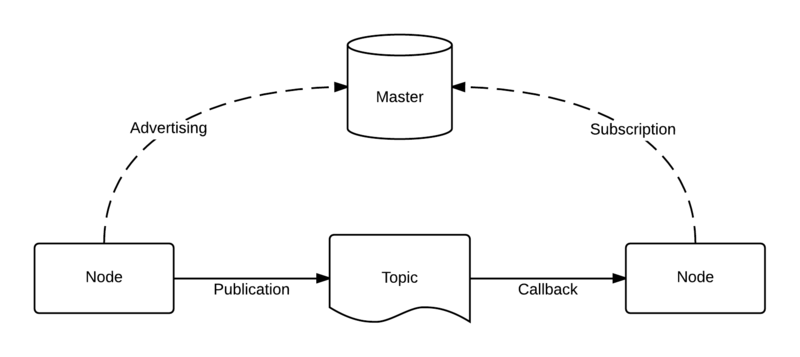
\includegraphics[width=0.8\textwidth]{gfx/master_node_topic}
    \caption[Funzionamento di \emph{master}, \emph{node} e \emph{topic} in \acs{ROS}.]{Funzionamento di \emph{master}, \emph{node} e \emph{topic} in \acs{ROS}.}
    \label{fig:master_node_topic}
\end{figure}

\subsection{Services}
I \emph{services} rappresentano il mezzo di comunicazione sincrono secondo una semantica di tipo request/reply (richiesta/risposta), implementando in \acs{ROS} una funzionalità di tipo \ac{RPC}. Pertanto, si definiscono nella rete nodi provider, che forniscono servizi, e nodi client, che usufruiscono di tali servizi.\\

Esistono funzioni per verificare la presenza di un service provider nella rete. Nel dettaglio, il nodo client invia dei dati che prendono il nome di request a un nodo server, aspettando la risposta di quest’ultimo. Il nodo server, una volta ricevuta, processa la request del client e gli riscontra dei dati in risposta (response).

\subsection{tf}
Quando si eseguono compiti con un robot, è fondamentale che il robot sia consapevole di dove si trova e di dove si trova il resto del mondo rispetto a se stesso. La libreria \emph{tf} \cite{tf} è stata progettata per fornire un modo standard per tenere traccia dei riferimenti di coordinate e trasformare i dati all'interno di un intero sistema in modo tale che gli utenti dei singoli componenti possano essere sicuri che i dati si trovino nel frame di coordinate desiderato, senza richiedere la conoscenza di tutti i riferimenti di coordinate nel sistema. Man mano che i sistemi robotici diventano sempre più complicati, essere in grado di concentrarsi con precisione sul task frame, cioè un frame di coordinate che può essere collegato a diversi oggetti che devono essere manipolati, e sui frame di coordinate rilevanti diventa fondamentale. La maggior parte dei sistemi robotici fonde i dati di molti sensori diversi con frame di coordinate differenti.\\

La libreria \emph{tf} è stata sviluppata come pacchetto \acs{ROS} per fornire questa capacità ed è composta da due moduli standard: un broadcaster (emittente) e un listener (ascoltatore). La prima parte si occupa della diffusione delle informazioni di trasformazione all'intero sistema. La seconda parte riceve le informazioni di trasformazione e le archivia per un uso successivo. Quindi è in grado di rispondere a domande sulla trasformazione risultante tra diversi frame di coordinate.\\

Le trasformazioni e i frame di coordinate possono essere espressi come un grafo con le trasformazioni come archi e i frame di coordinate come vertici. In questa rappresentazione la trasformata netta è semplicemente il prodotto degli archi che collegano due nodi qualsiasi. Il grafo può esistere con uno o più sottografi disconnessi e la trasformazione può essere calcolata tra nodi all'interno dei sottografi (intesi come componente connessa), ma non tra sottografi disconnessi. Tuttavia, in un grafo arbitrario, due nodi possono avere più cammini tra di loro, risultando in due o più potenziali trasformazioni nette che rendono ambiguo il risultato della query. Per evitare questo il grafo deve essere aciclico, in modo che ogni sottografo connesso è un albero. Limitare il grafo a un albero consente una rapida ricerca della connettività. Questo diventa importante con l'aumentare della complessità del grafo. Una struttura ad albero ha anche il vantaggio di consentire modifiche dinamiche alla struttura senza utilizzare informazioni aggiuntive rispetto agli archi del grafo diretto.\\

Il modulo broadcaster è stato progettato in modo molto semplice. Trasmette messaggi ogni volta che si verifica un aggiornamento su una trasformazione specifica.\\

Il modulo listener raccoglie i valori in un elenco ordinato e, quando interrogato, può interpolare tra i due valori più vicini. La frequenza di trasmissione delle trasformate da parte dell'emittente deve essere selezionata sufficientemente alta da consentire la \ac{SLERP} \cite{SLERP}.\\

Per calcolare le trasformazioni tra due nodi qualsiasi, viene calcolato il cosiddetto spanning set. Per calcolare lo spanning set tra un frame di origine e quello di destinazione, il modulo listener risale l'albero (attraverso la relazione di genitore) finché non viene trovato un nodo genitore comune che forma uno spanning set. Se non viene trovato alcun genitore comune, la ricerca fallisce e restituirà un errore. Se la ricerca ha esito positivo, il listener calcolerà la trasformazione netta degli archi dal frame di origine al frame di destinazione lungo il cammino percorso.

\subsection{RViz}
\ac{RViz} è uno strumento di visualizzazione 3D di \acs{ROS}. Consente di visualizzare il robot, il suo orientamento, i sistemi di riferimento, le matrici di covarianza e molto altro. Nell'ambito della tesi è risultato molto utile nelle simulazioni di volo per visualizzare in tempo reale la posizione del drone rispetto al sistema di riferimento a terra.

\begin{figure}[H]
	\begin{center}
	
	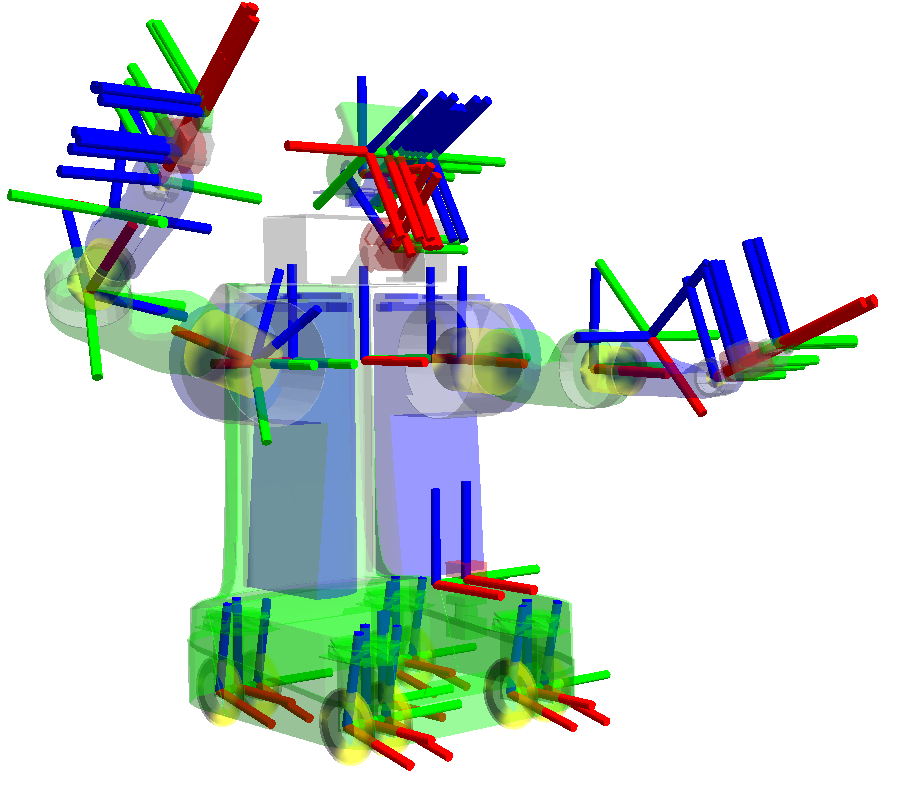
\includegraphics[width=0.5\textwidth]{gfx/tfROS}
    \caption[Task frames del robot PR2 di Willow Garage, in \acs{RViz}.]{Task frames nel robot PR2 di Willow Garage, visualizzate in \acs{RViz}. I cilindri RGB rappresentano gli assi X, Y e Z dei riquadri di coordinate.}
    \label{fig:tf_ROS}
    
    \vspace{30mm}

	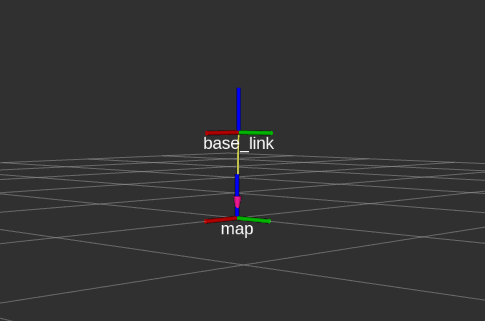
\includegraphics[width=0.5\textwidth]{gfx/ROS/rqt_rviz}
	\caption[Task frames del quadrirotore simulato, in \acs{RViz}.]{Task frames del quadrirotore simulato, visualizzate in \acs{RViz}. Il riferimento del sistema a terra è indicato con \emph{map}, quello solidale al quadrirotore con \emph{base\_link}.}
	\label{fig:droneRviz}
		
	\end{center}
\end{figure}

\pagebreak

% ------------------------------ ARCHITETTURA SIM ------------------------------
\section{Architettura di Simulazione}
In questa sezione si entra nel dettaglio dell'architettura di simulazione utilizzata in \acs{ROS}, partendo dalla scelta del sistema operativo. È stato utilizzato il sistema operativo Linux Ubuntu versione 20.04 (Focal Fossa) in quanto compatibile e consigliato per la versione \acs{ROS} adottata (Noetic Ninjemys, rilasciata a Maggio 2020).

\subsection{Gazebo}
Gazebo è un simulatore 3D. Consente di creare uno scenario tridimensionale sul computer con robot, ostacoli e altri oggetti utili alla simulazione del robot in questione.\\

In questo lavoro di tesi, si è fatto uso della repository \emph{iq\_sim} di Intelligent Quads, disponibile su GitHub \cite{iqSIM}. Questa repository contiene mondi gazebo per vari scenari e configurazioni di droni. Inoltre, è specificamente progettata per funzionare con il sistema di controllo ArduPilot e utilizza il plug-in gazebo ArduPilot per consentire al software di controllo ArduPilot di interfacciarsi e controllare il drone in gazebo.\\

Dopo aver clonato la repository sul computer utilizzato, per lanciare gazebo con il mondo desiderato basta eseguire da terminale il seguente comando.\\

\begin{lstlisting}[language=bash, numbers=none]
  roslaunch iq_sim runway.launch
\end{lstlisting}

\begin{figure}[H]
	\centering
	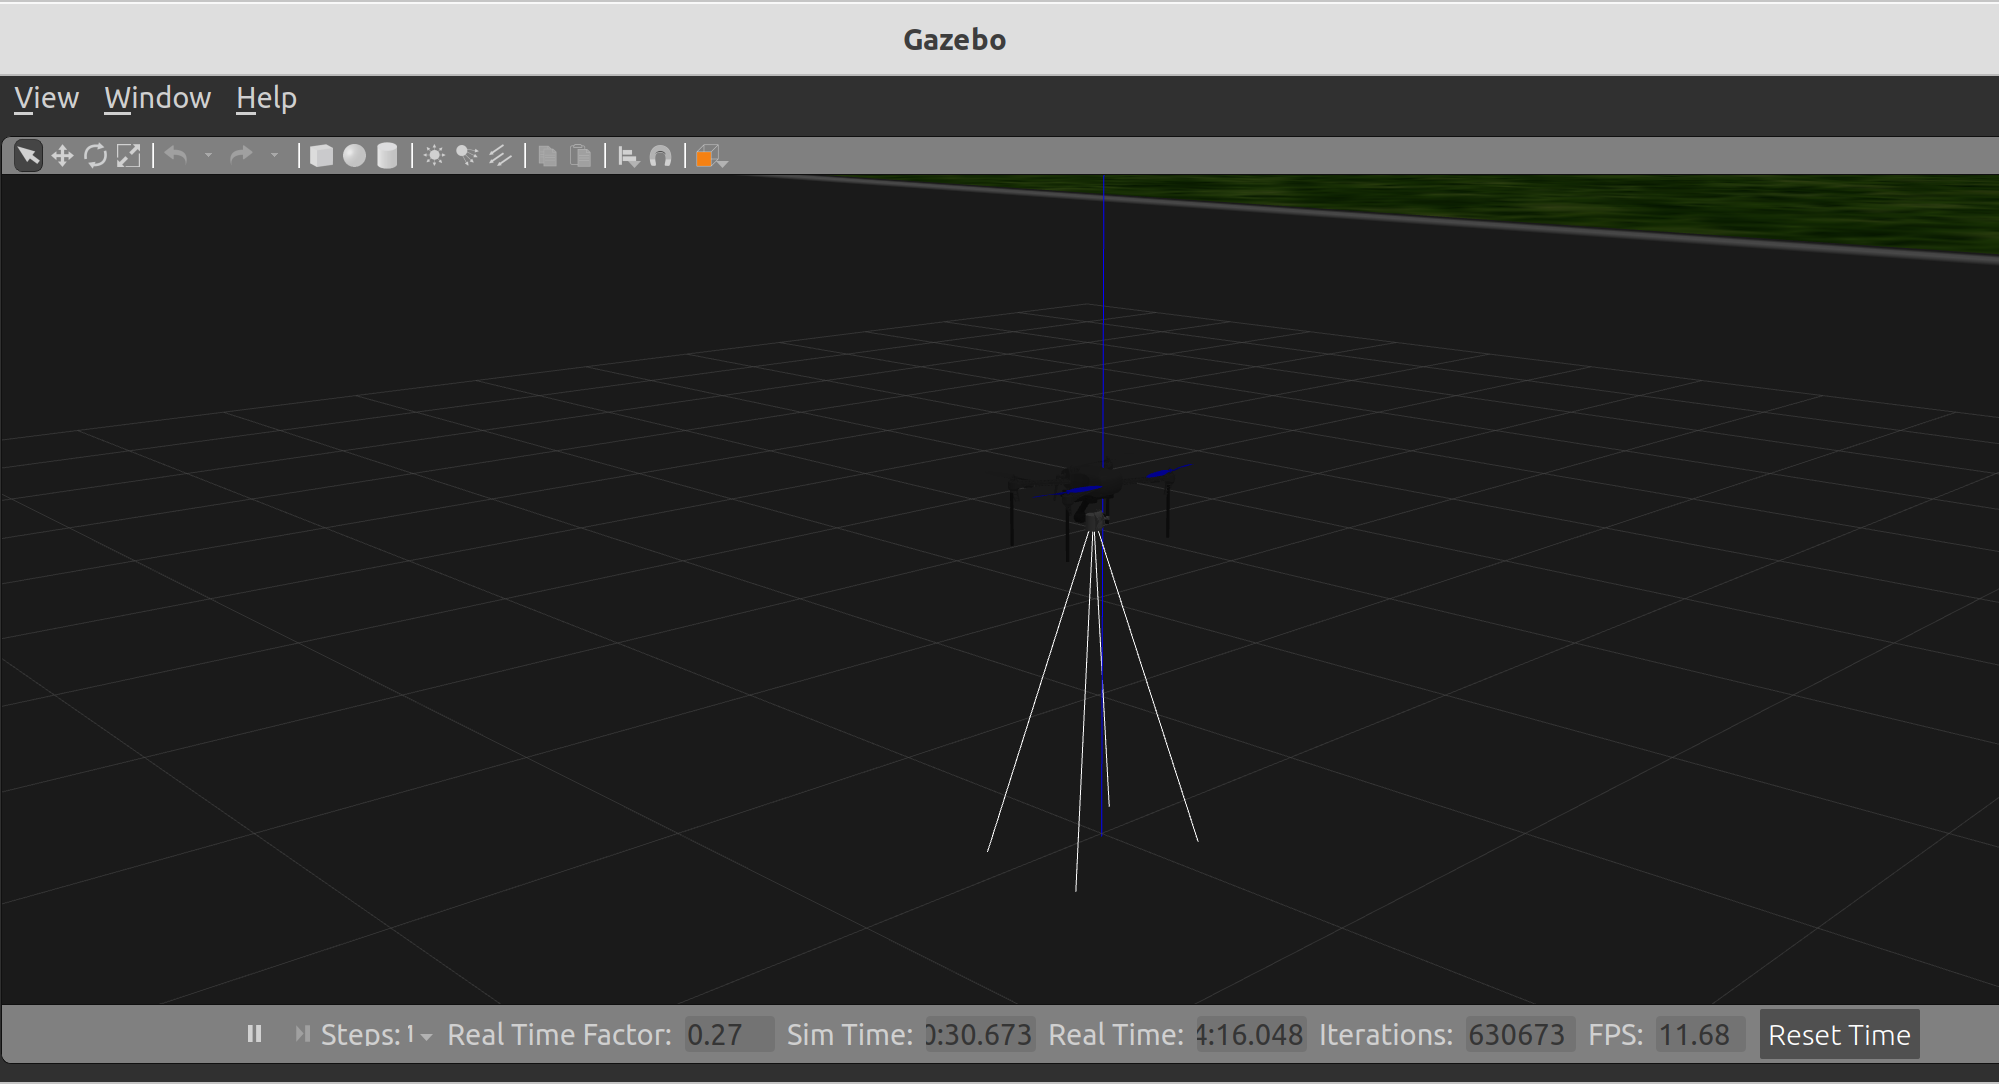
\includegraphics[width=0.75\textwidth]{gfx/ROS/gazebo_new}
	\caption[Quadrirotore nel mondo simulato.]{Quadrirotore nel mondo simulato \emph{runway.world} (pista di decollo) di Intelligent Quads, in Gazebo.}
	\label{fig:gazebo}
\end{figure}

\subsection{ArduCopter}
Gli aeromobili a pilotaggio remoto (\acs{UAV}) sono sistemi che richiedono una rapida risposta al variare dei dati forniti dai sensori a bordo, per cui risulta fondamentale per il controllo del volo un software di autopilotaggio. Esistono diverse soluzioni, ma per questa tesi è stato considerato il software ArduCopter, cioè la versione per \acs{UAV} del più generale software ArduPilot.\\

\ac{SITL} \cite{sitl} è un simulatore che consente di eseguire ArduCopter sul computer, senza l'utilizzo di alcun hardware. Per lanciare ArduCopter si esegue il seguente comando da terminale, assicurandosi di essere nella directory corretta di ArduPilot. Le Figure \ref{fig:arduCopter} e \ref{fig:consArduCopter} mostrano le interfacce grafiche contenenti tutte le informazioni sullo stato del velivolo e altri parametri.\\

\begin{lstlisting}[language=bash, numbers=none]
  ./sim_vehicle.py -v ArduCopter -f gazebo-iris --console --mavproxy-args="--streamrate=100"
\end{lstlisting}

\begin{figure}[H]
	\centering
	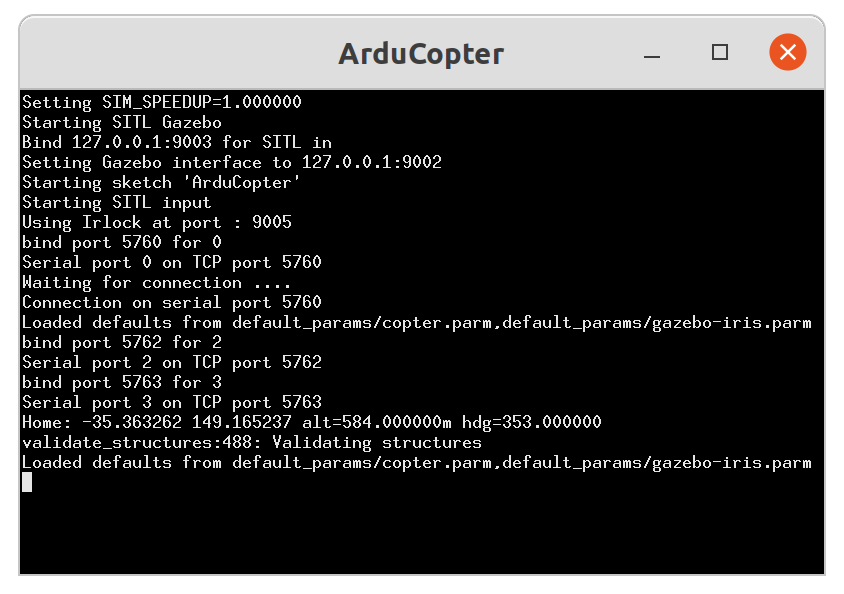
\includegraphics[width=0.65\textwidth]{gfx/ROS/ArduCopter}
	\caption[Interfaccia grafica ArduCopter.]{Interfaccia grafica ArduCopter.}
	\label{fig:arduCopter}
\end{figure}

\begin{figure}[H]
	\centering
	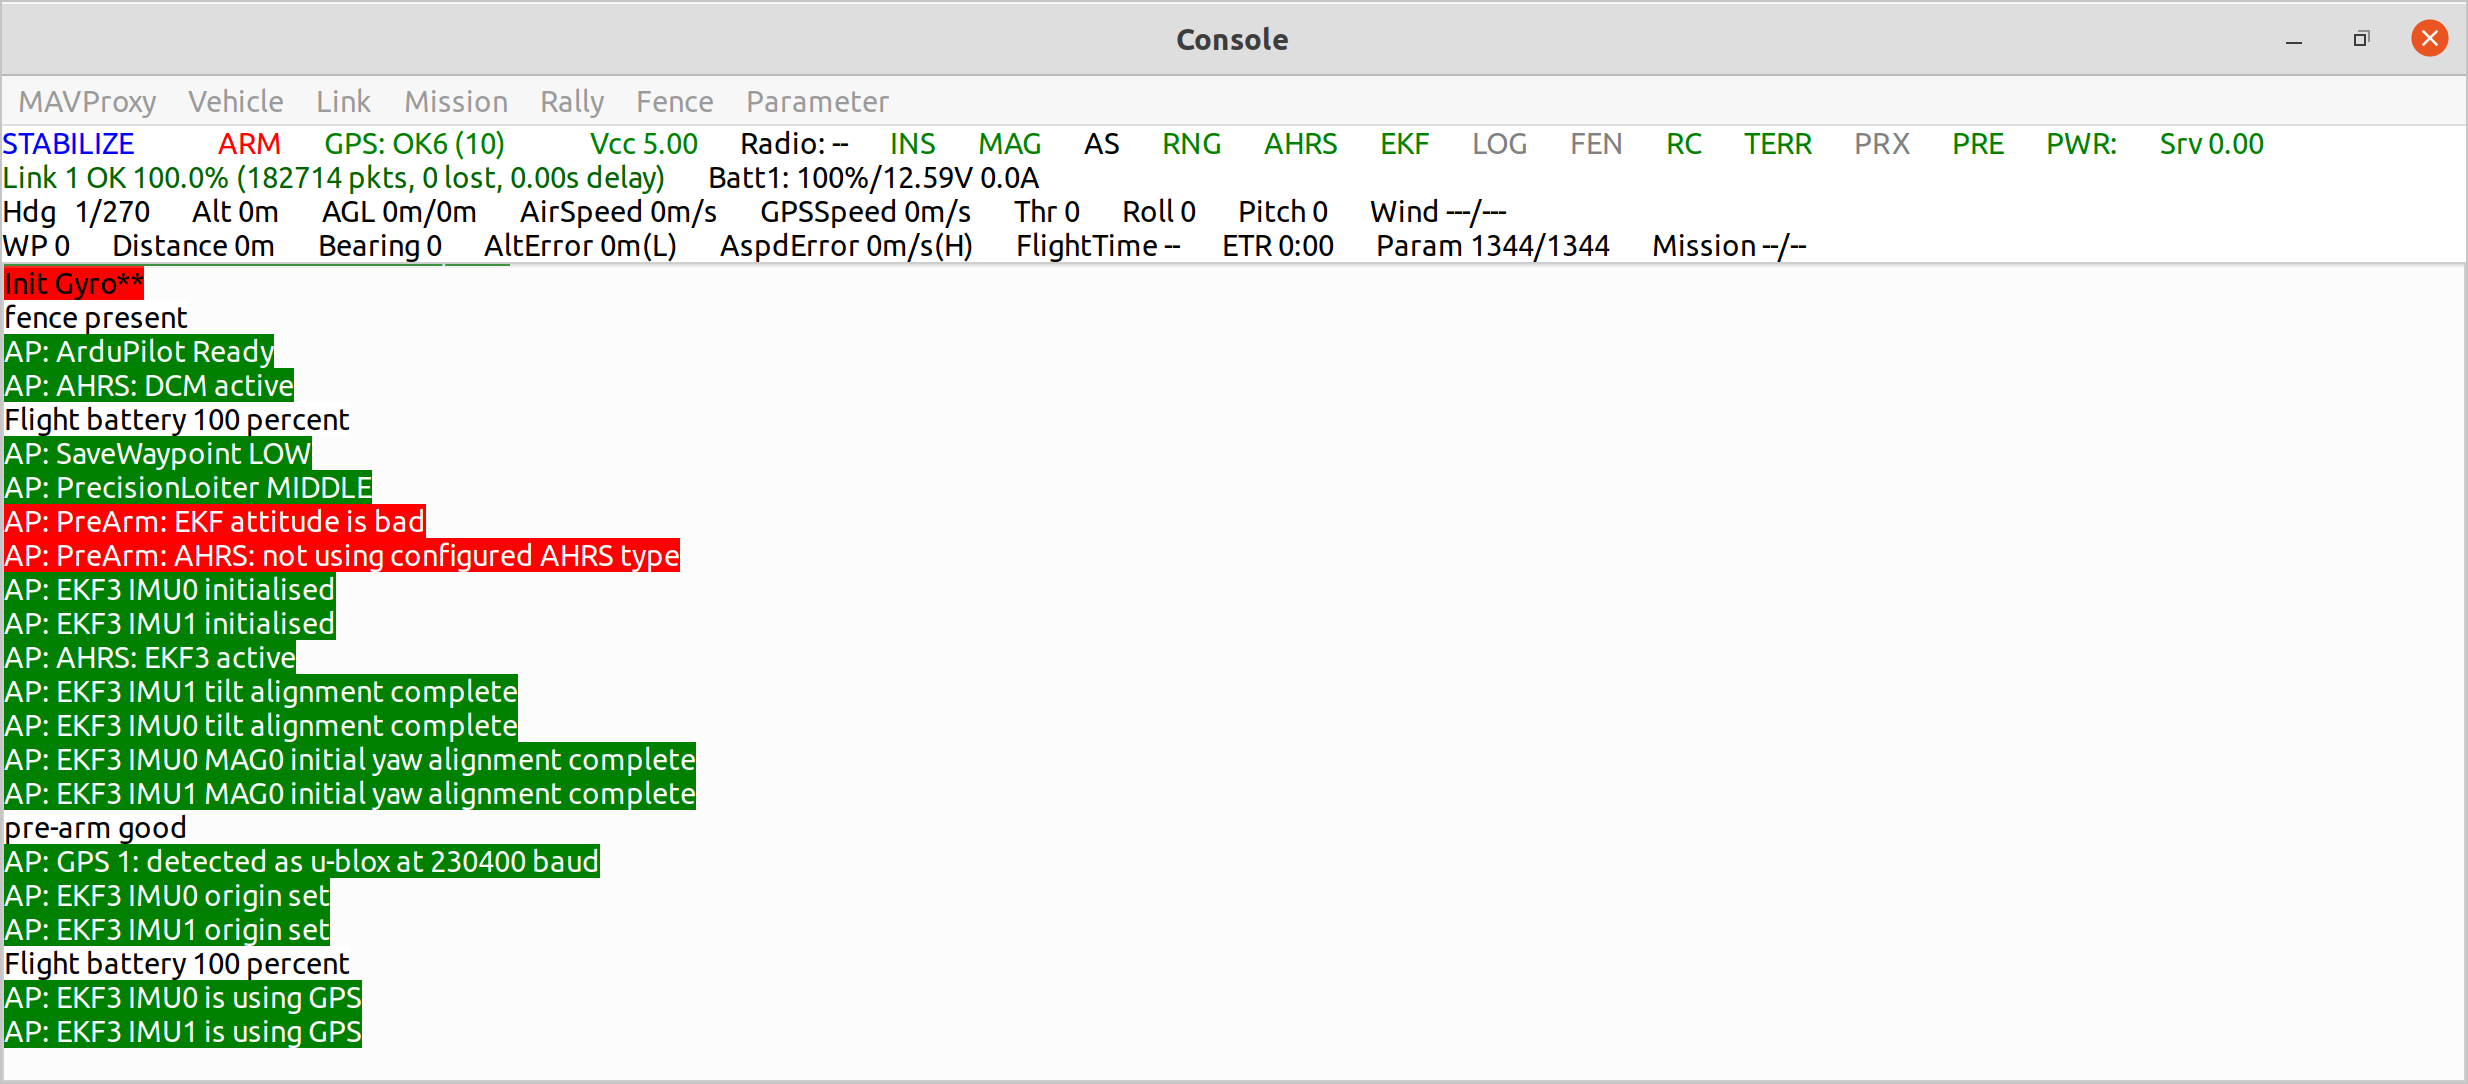
\includegraphics[width=1\textwidth]{gfx/ROS/SITL}
	\caption[Interfaccia grafica console ArduCopter.]{Interfaccia grafica console ArduCopter.}
	\label{fig:consArduCopter}
\end{figure}

\subsection{MAVLink e MAVROS}
MAVLink (Micro Air Vehicle Link) è un protocollo di comunicazione per \acs{UAV} di piccole dimensioni. I pacchetti utilizzati nella comunicazione MAVLink sono strutture in linguaggio C, trasmesse molto efficientemente attraverso dei canali di comunicazione seriale. I punti a suo favore sono sicuramente la velocità di comunicazione, la facilità con cui si possono realizzare nuovi messaggi e il fatto di essere open source. Per quanto riguarda la possibilità di creare nuovi messaggi, MAVLINK permette la definizione mediante file XML (chiamati dialetti), i quali vengono convertiti in codice sorgente in diversi linguaggi in base alle esigenze.\\

MAVROS \cite{mavros} è l'estensione di MAVLink in \acs{ROS}. Tra le tante caratteristiche di MAVROS vale la pena menzionare il fatto che è in grado di convertire i riferimenti di tipo \acs{NED} in riferimenti di tipo \acs{ENU} e viceversa, in modo da essere conforme allo standard adottato in \acs{ROS}.\\

Per completare la configurazione del sistema di simulazione si lancia il file \emph{apm.launch} con il seguente comando da terminale.\\

\begin{lstlisting}[language=bash, numbers=none]
  roslaunch mavros apm.launch
\end{lstlisting}

\vspace{5mm}

Questo si occupa di stabilire una connessione tra l'istanza \acs{ROS} in questione e il simulatore configurato precedentemente (Gazebo e ArduCopter). Una delle operazioni più rilevanti, svolta da questo eseguibile, è quella di inviare dati relativi ai \emph{tf} (task frames) coinvolti. In particolare, invia con una certa frequenza di trasmissione dati sui \emph{tf} in modo da mantenerli aggiornati in tempo reale. I \emph{tf} possono essere visualizzati non solo in \acs{RViz}, come mostra la Figura \ref{fig:droneRviz}, ma anche nell'albero dei \emph{tf} (tf\_tree), come mostra la Figura \ref{fig:tf_tree}.

\begin{figure}[H]
	\centering
	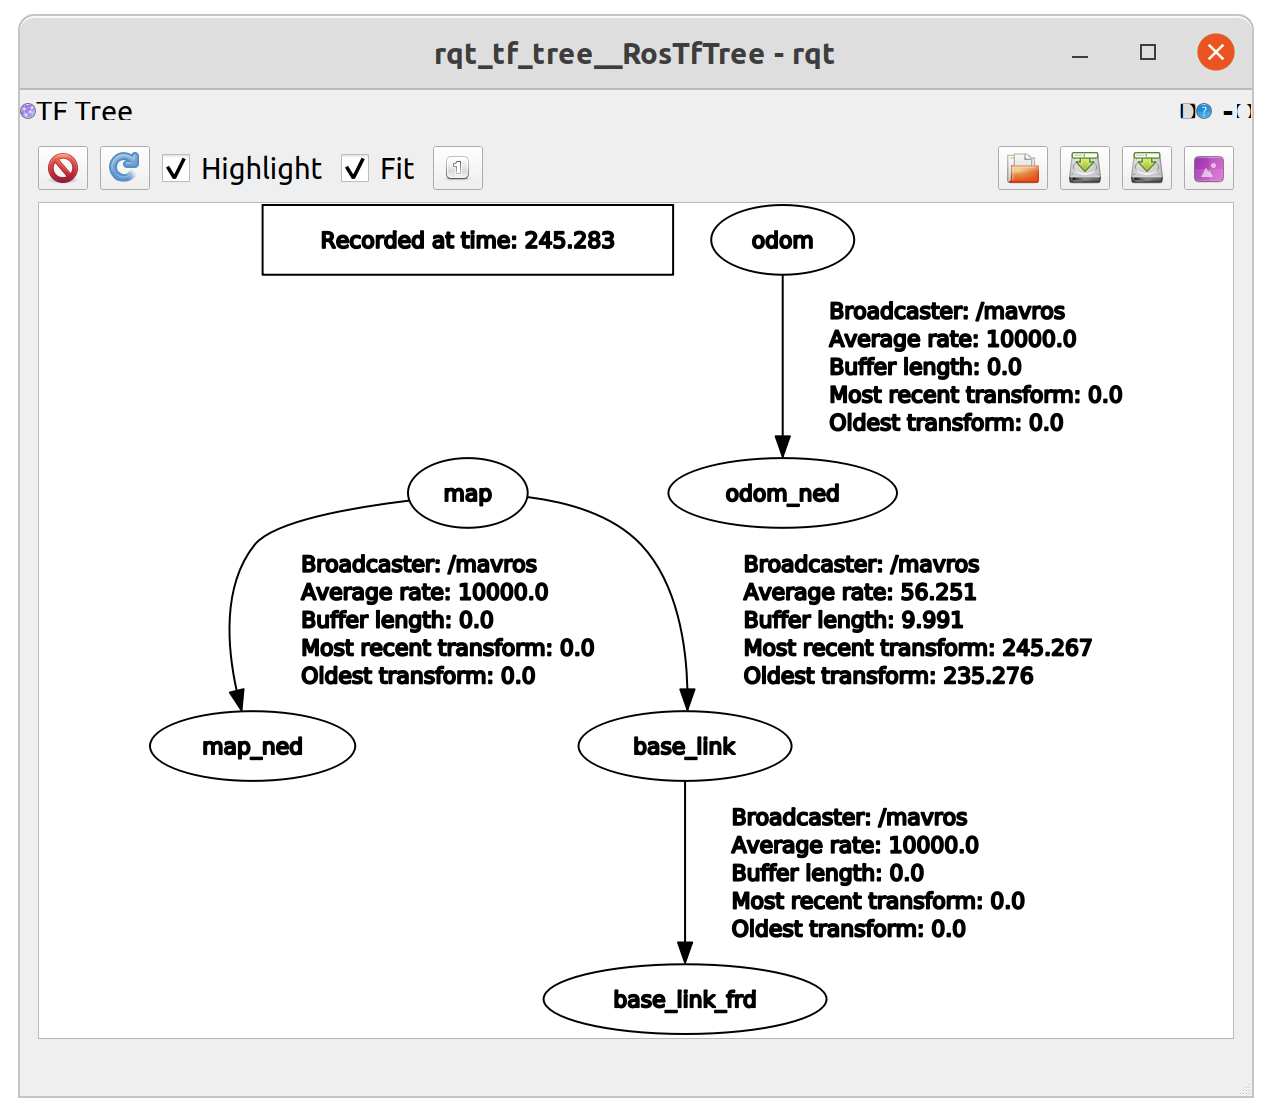
\includegraphics[width=0.75\textwidth]{gfx/ROS/rqt_tf_tree}
	\caption[Task frames del quadrirotore simulato, nel tf\_tree.]{Task frames del quadrirotore simulato, visualizzate nel tf\_tree. Il riferimento del sistema a terra è indicato con \emph{map}, quello solidale al quadrirotore con \emph{base\_link}.}
	\label{fig:tf_tree}
\end{figure}

% CHAPTER 4

\chapter{Identificazione}\label{ch:ident}
Data la crescente necessità di disporre di quadrirotori ad alte prestazioni, è necessario disporre di modelli accurati che descrivano al meglio il sistema reale, al fine di simulare ed implementare leggi di controllo ad alte prestazioni. Per questo motivo, il campo dell'identificazione di sistema è stato molto discusso negli ultimi decenni. In questo capitolo si cerca di identificare il modello dinamico di un quadrirotore.

% ------------------------------ INTRO ------------------------------

\section{Identificazione di Sistemi Dinamici}
L'identificazione di sistema consiste nella costruzione di modelli matematici partendo da dati sperimentali (input-output). Le tecniche di identificazione di sistema possono essere caratterizzate in termini di struttura del modello, tipo del modello e dominio dei dati input-output.\\

Esistono tre possibili tecniche di identificazione di sistema, che differiscono per quanto riguarda il grado di conoscenza e accesso al sistema oggetto di studio.\\

Il primo approccio è quello a scatola bianca (white box) e si applica quando si ha una conoscenza completa e dettagliata del sistema in esame. Si conoscono infatti tutte le equazioni matematiche e/o le leggi fisiche che governano il comportamento del sistema. Pertanto, l'identificazione del sistema si basa semplicemente sulla stima dei parametri delle equazioni conosciute, utilizzando dati sperimentali per ottimizzare o confermare il modello. Si tratta di una tecnica molto precisa, ma che richiede una conoscenza approfondita del sistema.\\

Il secondo approccio è quello a scatola grigia (gray box) e si applica quando si ha una conoscenza parziale del sistema in esame. Potrebbe essere noto solo un sottoinsieme delle equazioni o dei dettagli del sistema, mentre altri aspetti sono sconosciuti o approssimati. L'idea è quella di combinare la conoscenza parziale con dati sperimentali per costruire un modello che rappresenti accuratamente il sistema. Questo approccio è utile quando non si dispone di una comprensione completa del sistema, ma si hanno alcune informazioni chiave.\\

Il terzo approccio è quello a scatola nera (black box) e si applica quando non si ha conoscenza delle equazioni o dei dettagli interni del sistema. Il sistema viene trattato appunto come una scatola nera in cui si osservano le relazioni tra l'input e l'output, ma non si cerca di comprendere il funzionamento interno. L'obiettivo è identificare un modello empirico o una funzione di trasferimento (come si vedrà nel seguito) che descriva il comportamento del sistema basandosi solo su dati sperimentali. Questo approccio è utilizzati quando il sistema è molto complesso o non è possibile ottenere informazioni dettagliate sul suo funzionamento.\\

In questa tesi si utilizzerà MATLAB System Identification Toolbox \cite{sysID}, uno strumento fornito da MATLAB per l'identificazione di sistemi dinamici. Questo, tramite un'interfaccia grafica intuitiva, consente di inserire dati input-output e identificare il sistema secondo l'approccio black box. Le tre principali funzioni del tool sono le seguenti:
\begin{enumerate}
	\item \textbf{Data Preprocessing}. I dati input-output registrati possono essere elaborati in vario modo. Ad esempio possono essere filtrati, possono essere trasformati in segnali a media nulla oppure si può ridurre la finestra di interesse ad un determinato intervallo temporale. Queste tecniche sono molto utili in quanto i dati, così come sono stati raccolti, non sempre sono sufficienti per identificare un modello accurato.
	\item \textbf{System Identification}. Esistono numerosi tipi di modelli identificabili. Si possono identificare sia modelli \ac{SISO} che modelli \ac{MIMO}.
	\item \textbf{System Validation}. Una volta identificato il modello si è interessati a capire se il suo comportamento è effettivamente simile (ed eventualmente quanto) a quello reale. MATLAB fornisce una funzione che simula la risposta del modello identificato (inserendo nel sistema l'input misurato) e la sovrappone all'uscita misurata \cite{compare}. Inoltre, mostra anche la misura del \ac{NRMSE}, che descrive la bontà dell'adattamento tra la risposta simulata e i dati di misurazione di output ed è definito come mostra la \ref{nrmse}.
\end{enumerate}

\begin{equation}
	RMSE = \sqrt{\frac{\sum_{i=1}^{n} {(\hat{y_i} - y_i)}^2}{n}}
	\label{rmse}
\end{equation}

\begin{equation}
	NRMSE = \frac{RMSE}{y_{max} - y_{min}}
	\label{nrmse}
\end{equation}

% ------------------------------ SIM FLIGHTS ------------------------------

\section{Simulazioni di Volo}
Per poter identificare al meglio il sistema del quadrirotore, è necessario effettuare delle simulazioni di volo che siano in grado di descrivere i singoli aspetti della dinamica del sistema. Il sistema di simulazione configurato è assolutamente privo di controllo, quindi è impossibile effettuare una traiettoria di volo desiderata agendo direttamente sugli angoli di Eulero.\\

\subsection{Controllore di Posizione}
Si è deciso di utilizzare un controllore, fornito già implementato, in grado di mantenere il drone in stato di hovering una volta decollato e in grado di farlo muovere verso uno specifico punto dello spazio. Il controllore è un pacchetto \acs{ROS} contenente nodi (Python) di varia utilità. Alcuni nodi gestiscono l'algoritmo matematico di controllo, altri si occupano di presentare all'utente un'interfaccia grafica per controllare lo spostamento del drone. Come mostra Figura \ref{fig:drone_controller}, l'utente può effettuare le seguenti operazioni, che corrispondo a servizi \acs{ROS} nel codice sorgente:
\begin{itemize}
	\item \textbf{Take Off} fa decollare il drone all'altezza specificata e lo stabilizza (stato di hovering);
	\item \textbf{Go To Point} imposta il setpoint da raggiungere verso le coordinate specificate (rispetto al sistema di rifierimento specificato, che può essere sia quello a terra che quello solidale al velivolo);
	\item \textbf{Go Home} riporta il drone nelle componenti del piano XY iniziali in cui è avvenuto il decollo;
	\item \textbf{Land} fa atterrare il drone, disarmando i motori.
\end{itemize}

\begin{figure}[H]
	\centering
	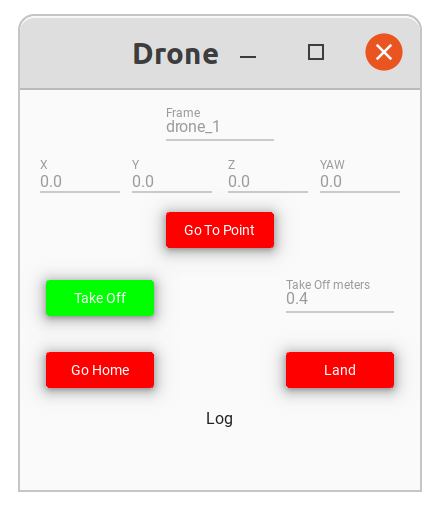
\includegraphics[width=0.43\textwidth]{gfx/ROS/drone_controller}
	\caption[Interfaccia grafica del controllore.]{Interfaccia grafica del controllore.}
	\label{fig:drone_controller}
\end{figure}

\subsection{Registrazione e Memorizzazione Dati}
I dati di interesse sono gli angoli di Eulero e la forza di spinta per quanto riguarda gli input, mentre le coordinate di posizione per quanto riguarda gli output. Per registrare e memorizzare queste informazioni sono state aggiunte alcune righe di codice in alcuni nodi del controllore. In particolare, per la gestione dei dati sono state utilizzate le librerie NumPy \cite{numPy} e SciPy \cite{sciPy}.\\

Prima di tutto sono stati inizializzati sette array NumPy (quattro per gli input e tre per gli output), poi sono stati riempiti all'interno del ciclo di controllo del drone utilizzando la funzione \emph{append()}, fornita dalla libreria NumPy. Il ciclo di controllo viene aggiornato con una frequenza di 100 Hz, quindi, al termine di una simulazione di volo ogni array sarà un segnale del tempo campionato con tempo di campionamento pari a 0.01 secondi. Il numero di campioni dipende dalla durata della simulazione e, ovviamente, tanto più è grande tanto più sarà precisa l'identificazione del modello. Ipotizzando che ogni volo registrato è durato in media due minuti, ogni segnale è caratterizzato da circa 12000 campioni. Sono state effettuate dieci simulazioni di volo in modo da poter identificare più modelli relativi a distinti insiemi di dati e confrontarli tra loro.\\

Per trasferire i dati registrati in MATLAB, dove poi avvengono i tre passi necessari per identificare e validare il sistema, si è fatto uso della funzione \emph{savemat()} della libreria di input-output di SciPy (\emph{scipy.io}).

% ------------------------------ SISO ------------------------------

\section{Identificazione Modelli SISO}
L'obiettivo di questa sezione è quello di identificare delle funzioni di trasferimento tempo continue, nel dominio di Laplace, che descrivano alcuni aspetti della dinamica del quadrirotore. Infatti, dato che i segnali di input coinvolti nella dinamica del sistema sono quattro ($\phi, \theta, \psi, U1$), si può disaccoppiare il sistema (\acs{MIMO}) in quattro sottosistemi identificabili separatamente (\acs{SISO}).\\

\subsection{Funzione di Trasferimento angolo di Rollio e posizione lungo Y}
I dati utilizzati per identificare la dinamica del velivolo lungo l'asse Y sono il segnale che descrive le variazioni dell'angolo di rollio (input) e il segnale che descrive le variazioni di posizione lungo lo stesso asse (output). Entrambi i segnali si presentano già a media nulla, quindi l'unica operazione di preprocessing effettuata è stata quella di considerare uno specifico intervallo temporale (dove il segnale è significativo). I segnali utilizzati sono mostrati in Figura \ref{fig:ry_input}.

\begin{figure}[H]
	\centering
	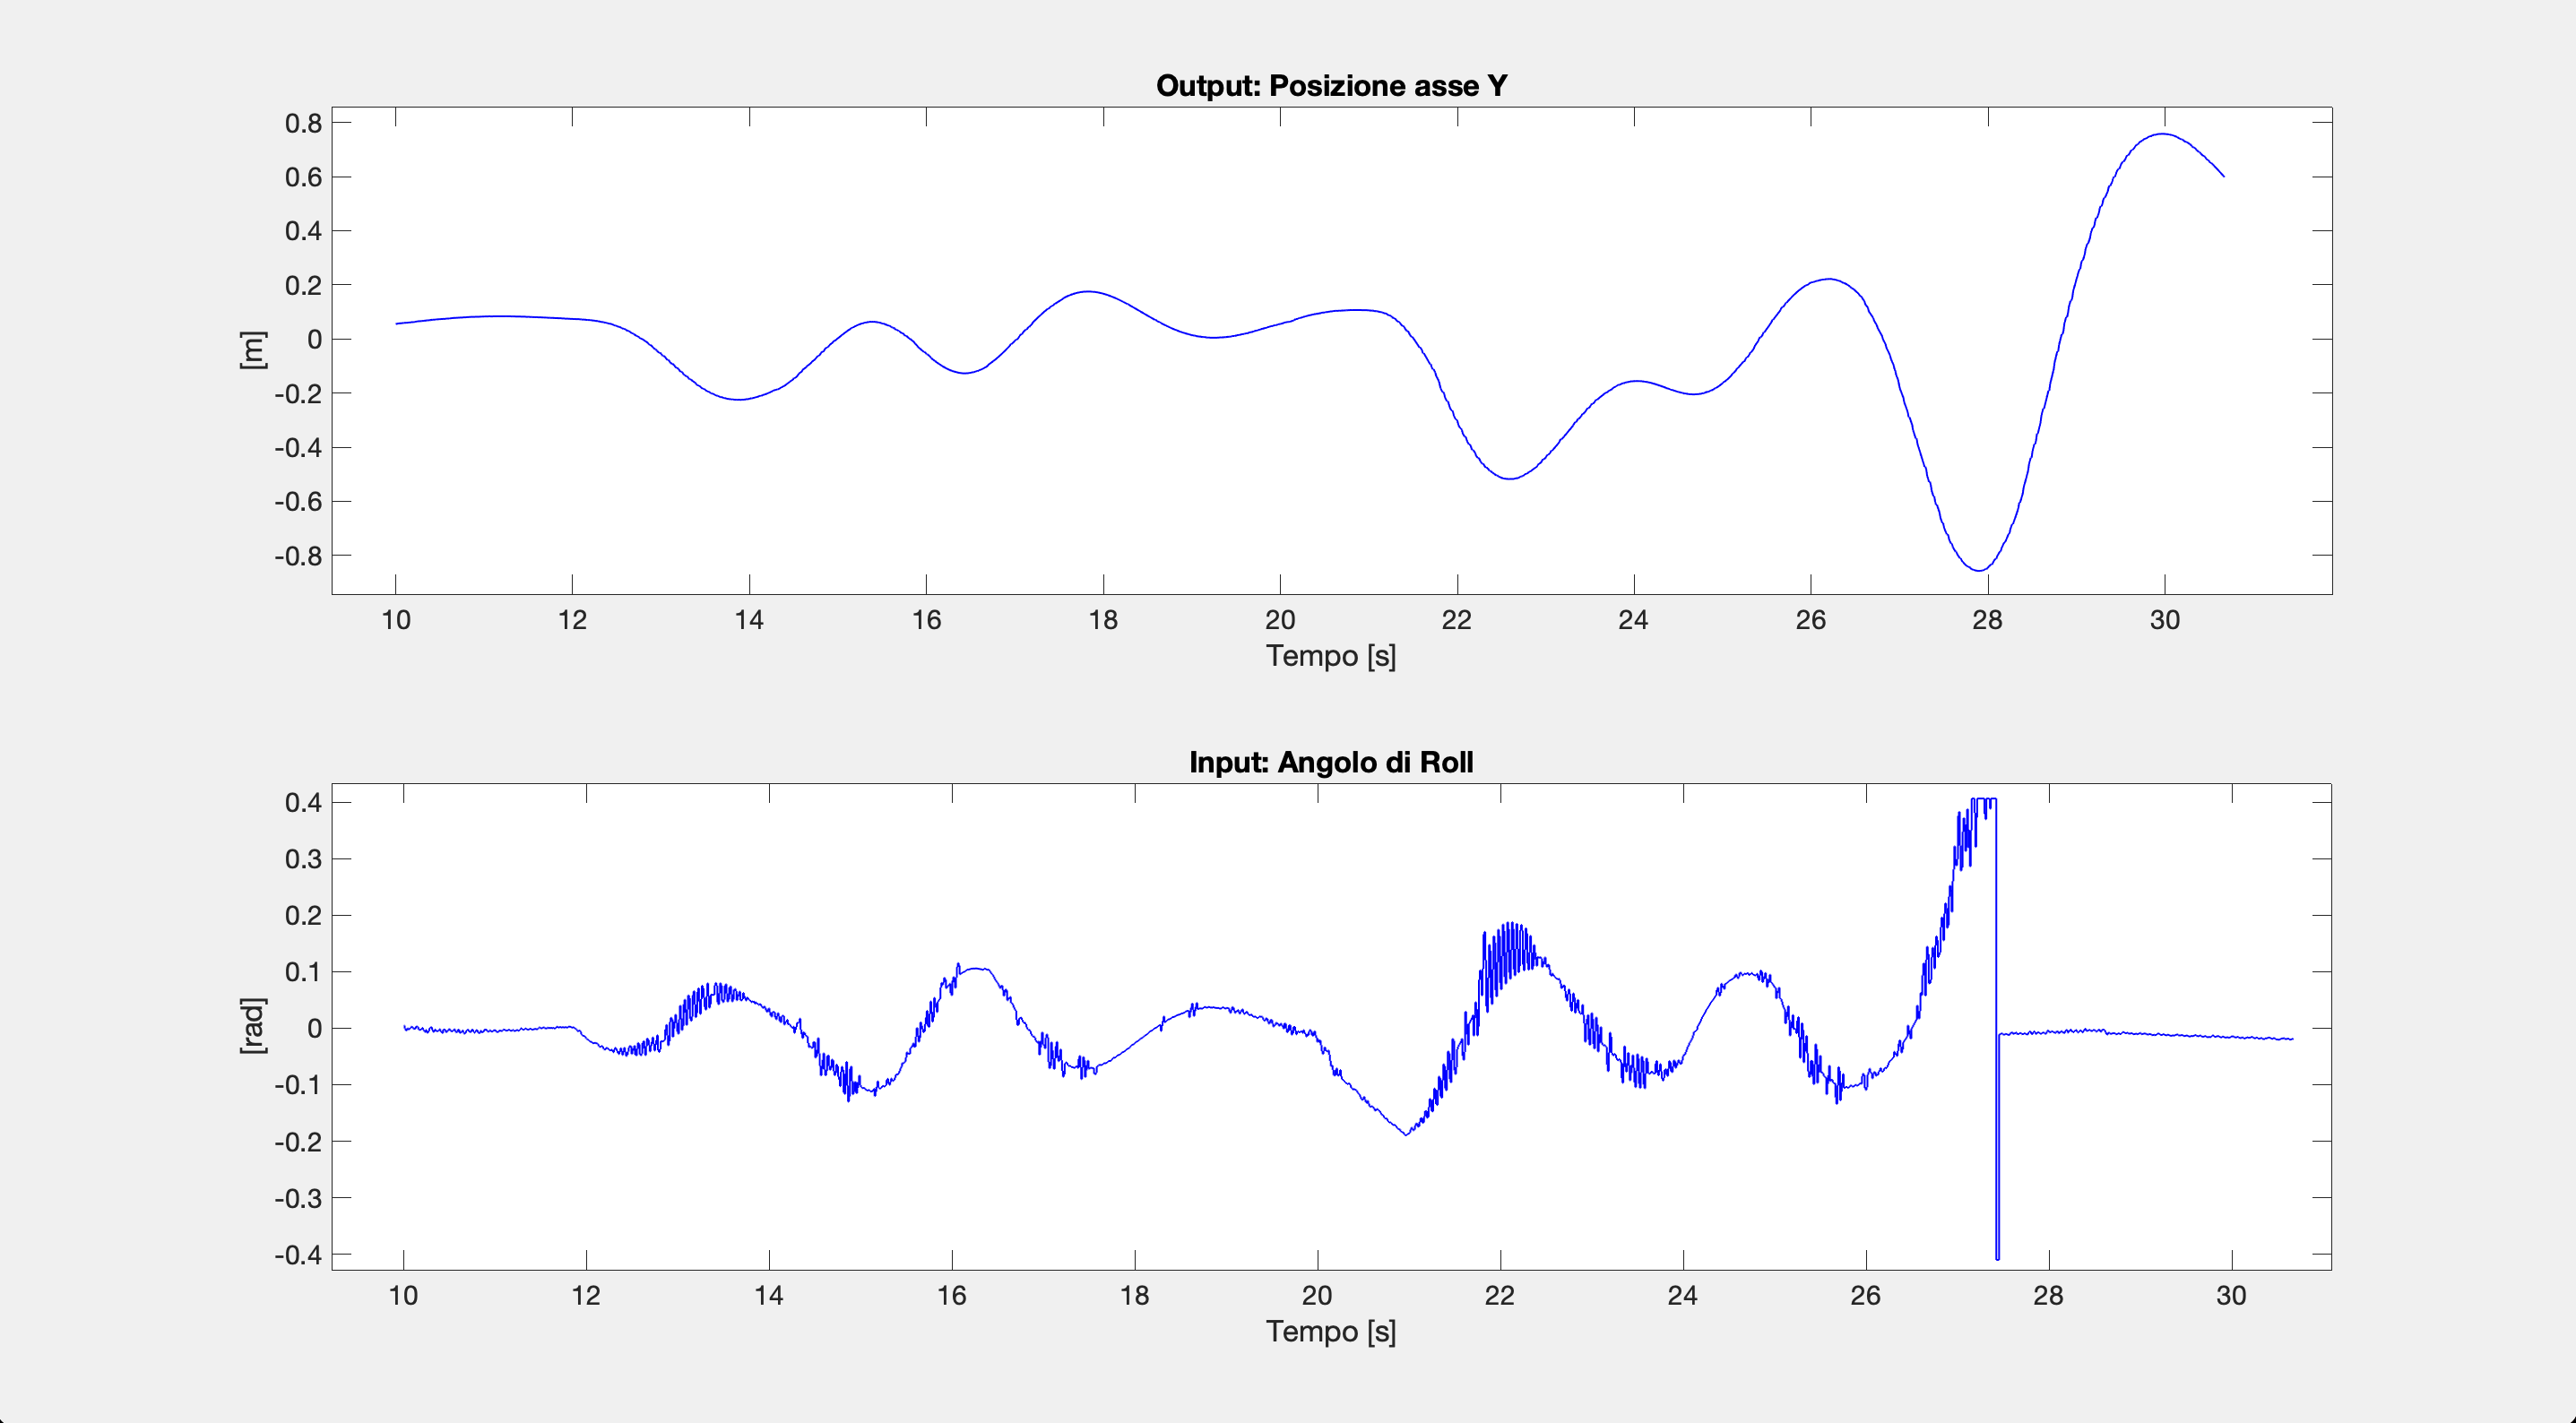
\includegraphics[width=1\textwidth]{gfx/SysId/ry_input}
	\caption[Dati input-output per identificare la dinamica del rollio.]{Dati input-output per identificare la dinamica del rollio. Input: variazione dell'angolo di rollio nel tempo. Output: variazione della posizione lungo l'asse Y nel tempo.}
	\label{fig:ry_input}
\end{figure}

La funzione di trasferimento identificata che lega l'angolo di rollio (roll) allo spostamento del velivolo lungo l'asse Y è la seguente (\ref{fdtY}).

\begin{equation}
	W_Y(s) = \frac{-1.022s^2 + 0.6857s + 1.873}{s^3 + 0.008794s^2 + 1.456s + 0.001566}
	\label{fdtY}
\end{equation}

Si tratta di un sistema lineare tempo continuo del terzo ordine (tre poli).\\

Completata la fase di identificazione, si passa alla terza e ultima fase, cioè la validazione del sistema. La funzione \emph{compare()} \cite{compare} mostra una buona compatibilità del modello identificato con quello reale, come mostra Figura \ref{fig:ry_model}. Il \acs{NRMSE} risulta in un 71.3\% di compatibilità.

\begin{figure}[H]
	\centering
	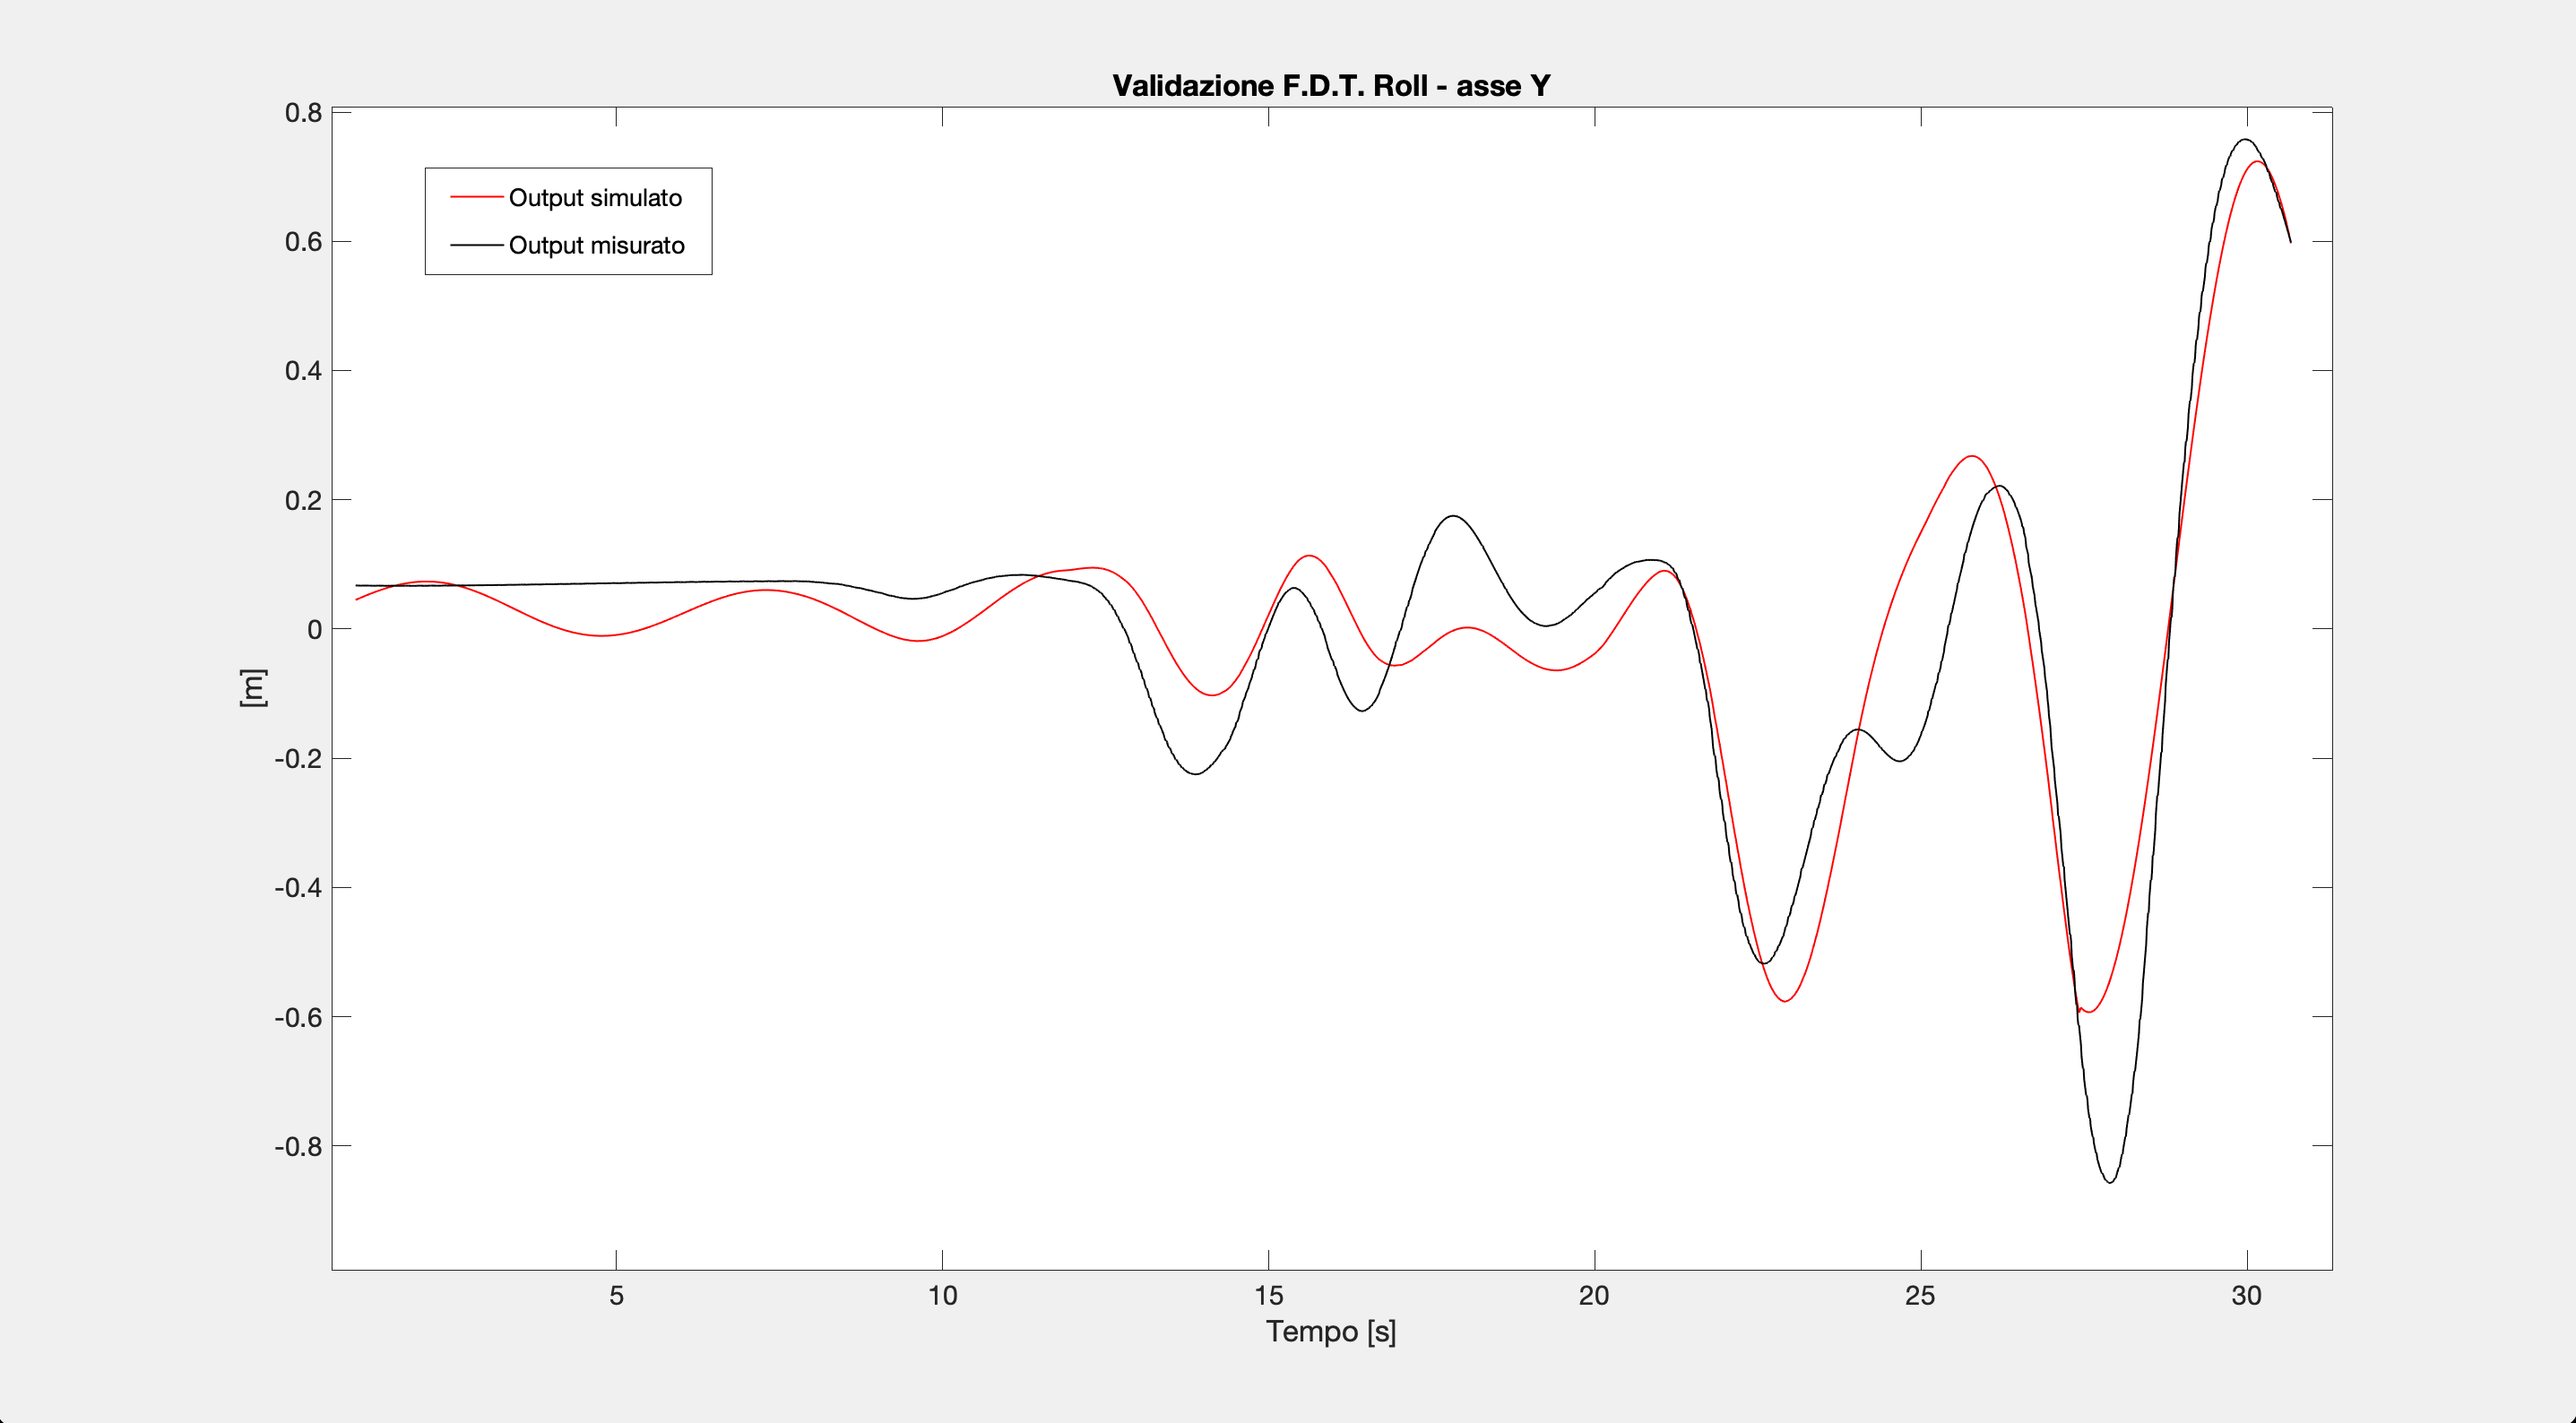
\includegraphics[width=1\textwidth]{gfx/SysId/ry_model}
	\caption[Validazione F.D.T. Roll - asse Y.]{Validazione F.D.T. Roll - asse Y.}
	\label{fig:ry_model}
\end{figure}

\subsection{Funzione di Trasferimento angolo di Beccheggio e posizione lungo X}
I dati utilizzati per identificare la dinamica del velivolo lungo l'asse X sono il segnale che descrive le variazioni dell'angolo di beccheggio (input) e il segnale che descrive le variazioni di posizione lungo lo stesso asse (output). Anche qui, entrambi i segnali si presentano già a media nulla, quindi l'unica operazione di preprocessing effettuata è stata quella di considerare uno specifico intervallo temporale (dove il segnale è significativo). I segnali utilizzati sono mostrati in Figura \ref{fig:px_input}.

\begin{figure}[H]
	\centering
	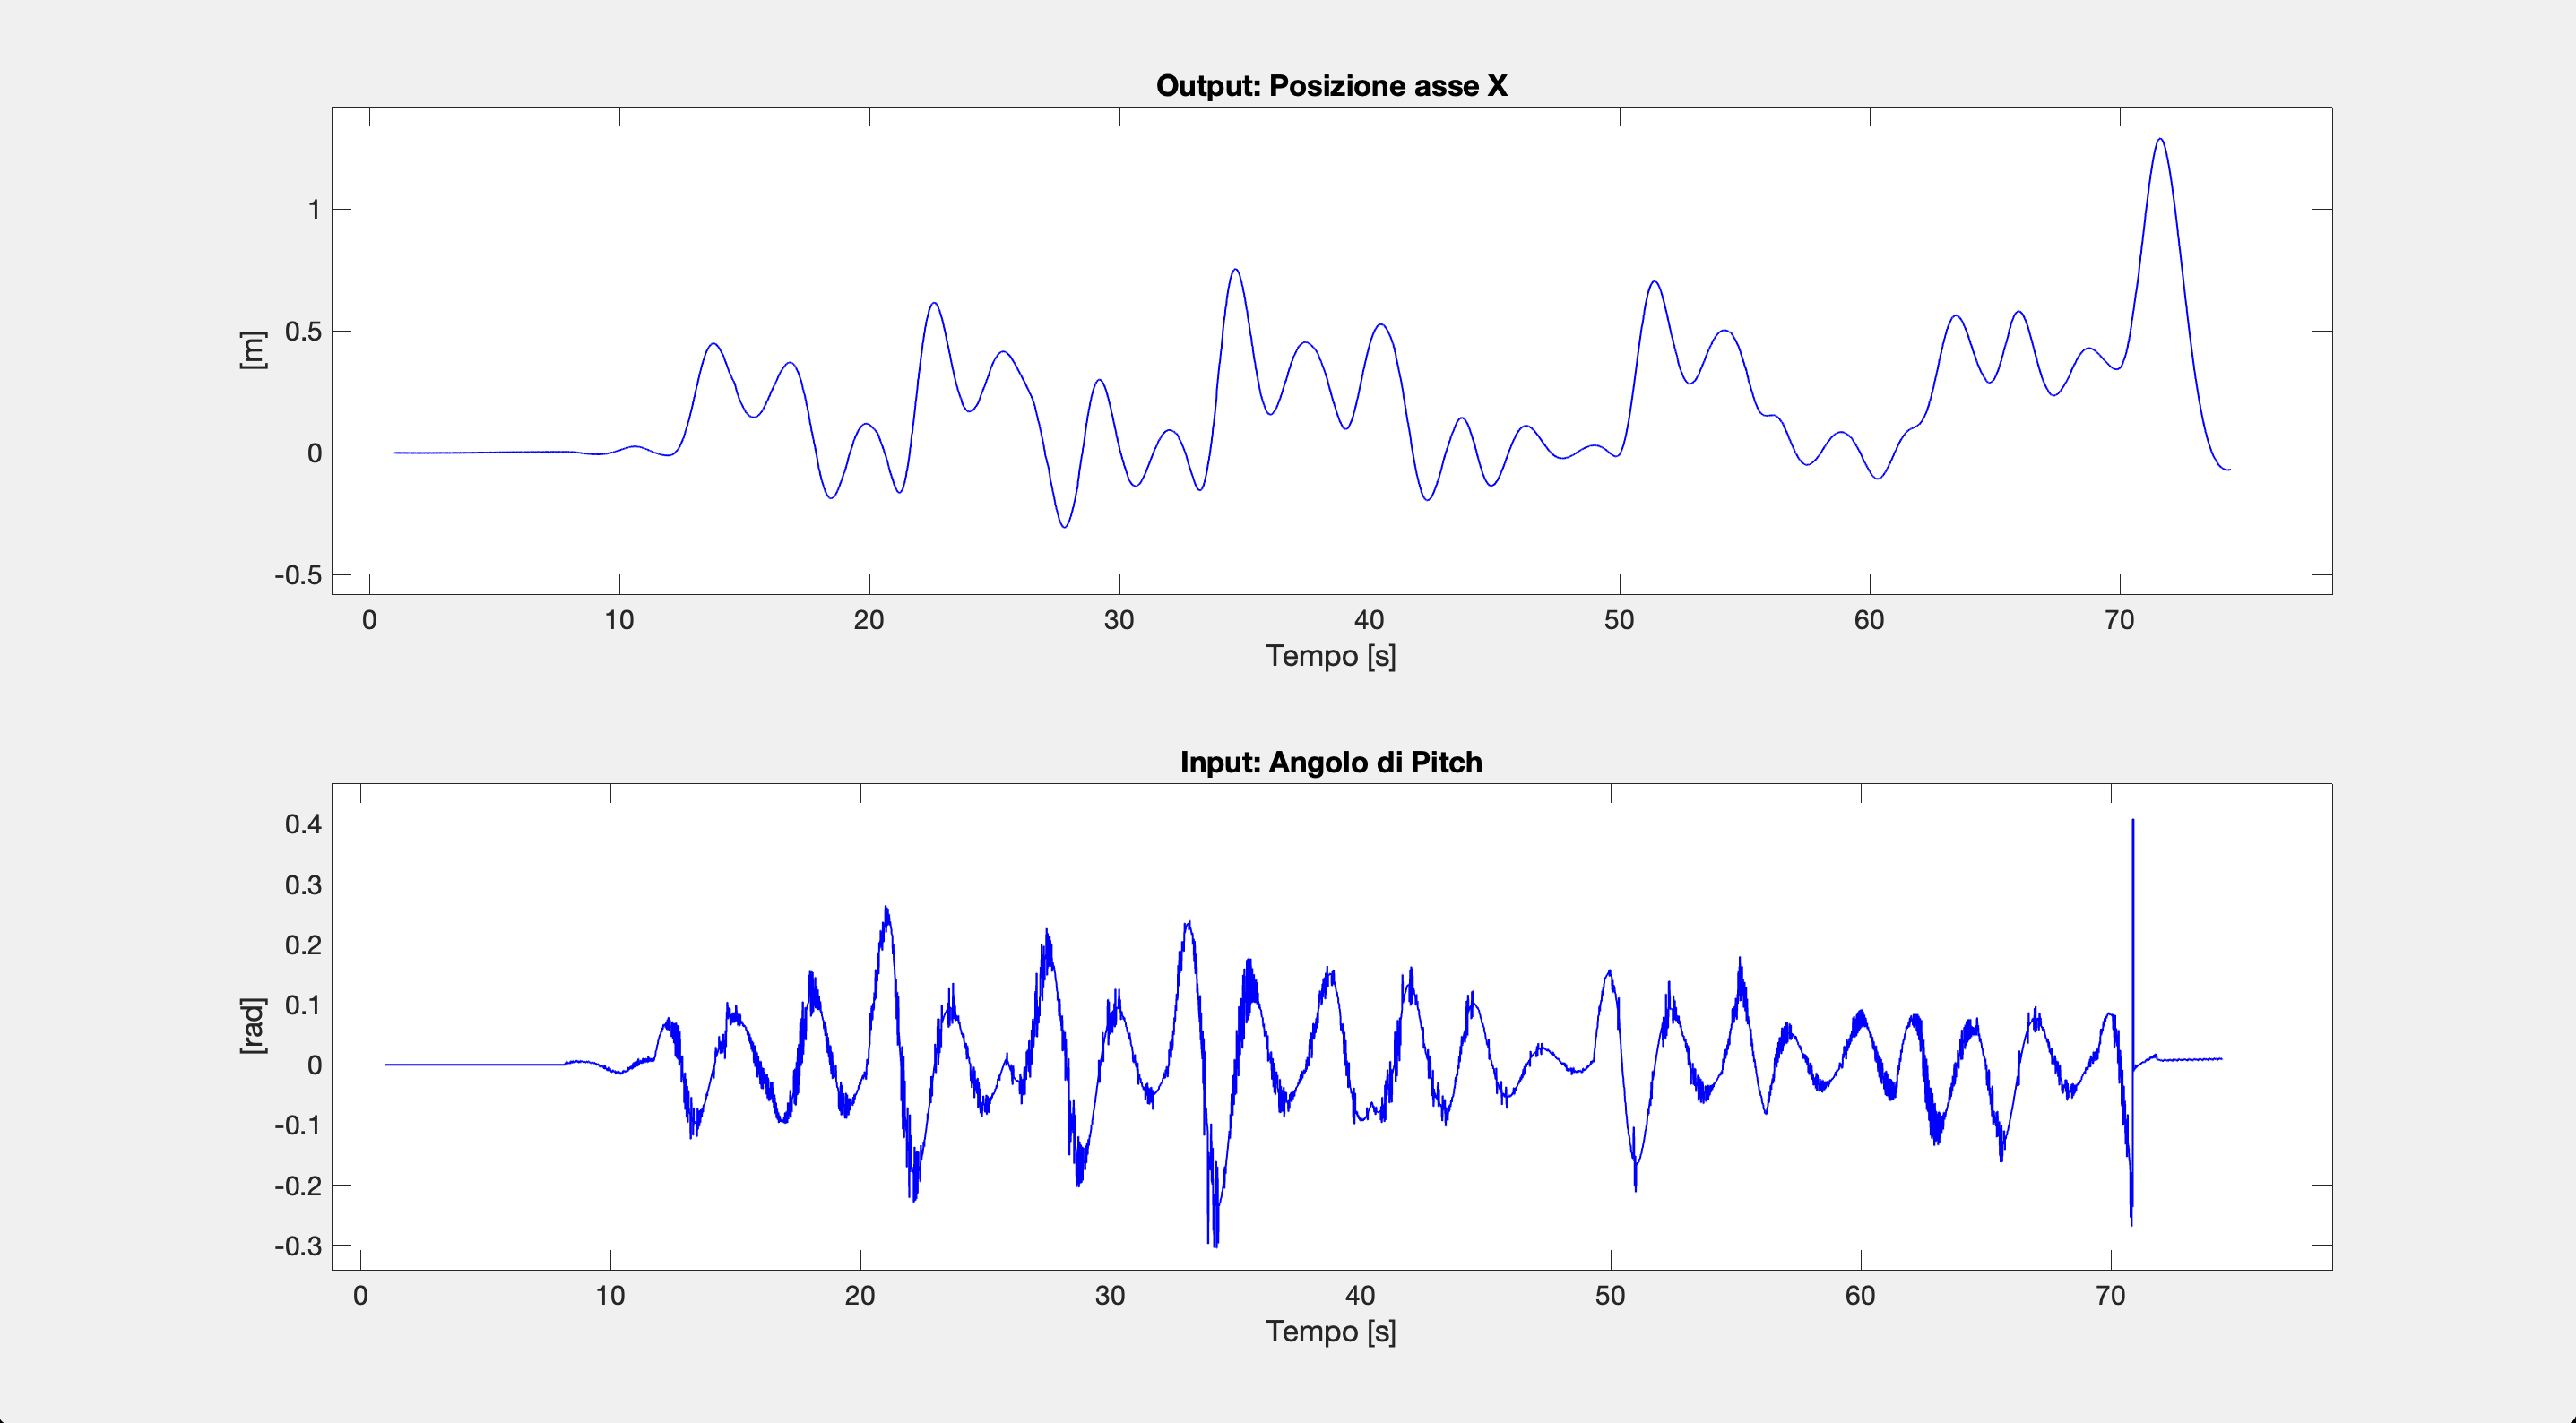
\includegraphics[width=1\textwidth]{gfx/SysId/px_input}
	\caption[Dati input-output per identificare la dinamica del beccheggio.]{Dati input-output per identificare la dinamica del beccheggio. Input: variazione dell'angolo di beccheggio nel tempo. Output: variazione della posizione lungo l'asse X nel tempo.}
	\label{fig:px_input}
\end{figure}

La funzione di trasferimento identificata che lega l'angolo di beccheggio (pitch) allo spostamento del velivolo lungo l'asse X è la seguente (\ref{fdtX}).

\begin{equation}
	W_X(s) = \frac{-3.224s^2 + 3.491s + 1.71}{s^3 + 1.16s^2 + 0.1916s + 0.1929}
	\label{fdtX}
\end{equation}

Anche in questo caso si ottiene un sistema lineare tempo continuo del terzo ordine (tre poli).\\

Per quanto riguarda la validazione, la funzione \emph{compare()} \cite{compare} mostra ancora una buona compatibilità del modello identificato con quello reale, come mostra Figura \ref{fig:px_model}. Il \acs{NRMSE} risulta in un 69.7\% di compatibilità.

\begin{figure}[H]
	\centering
	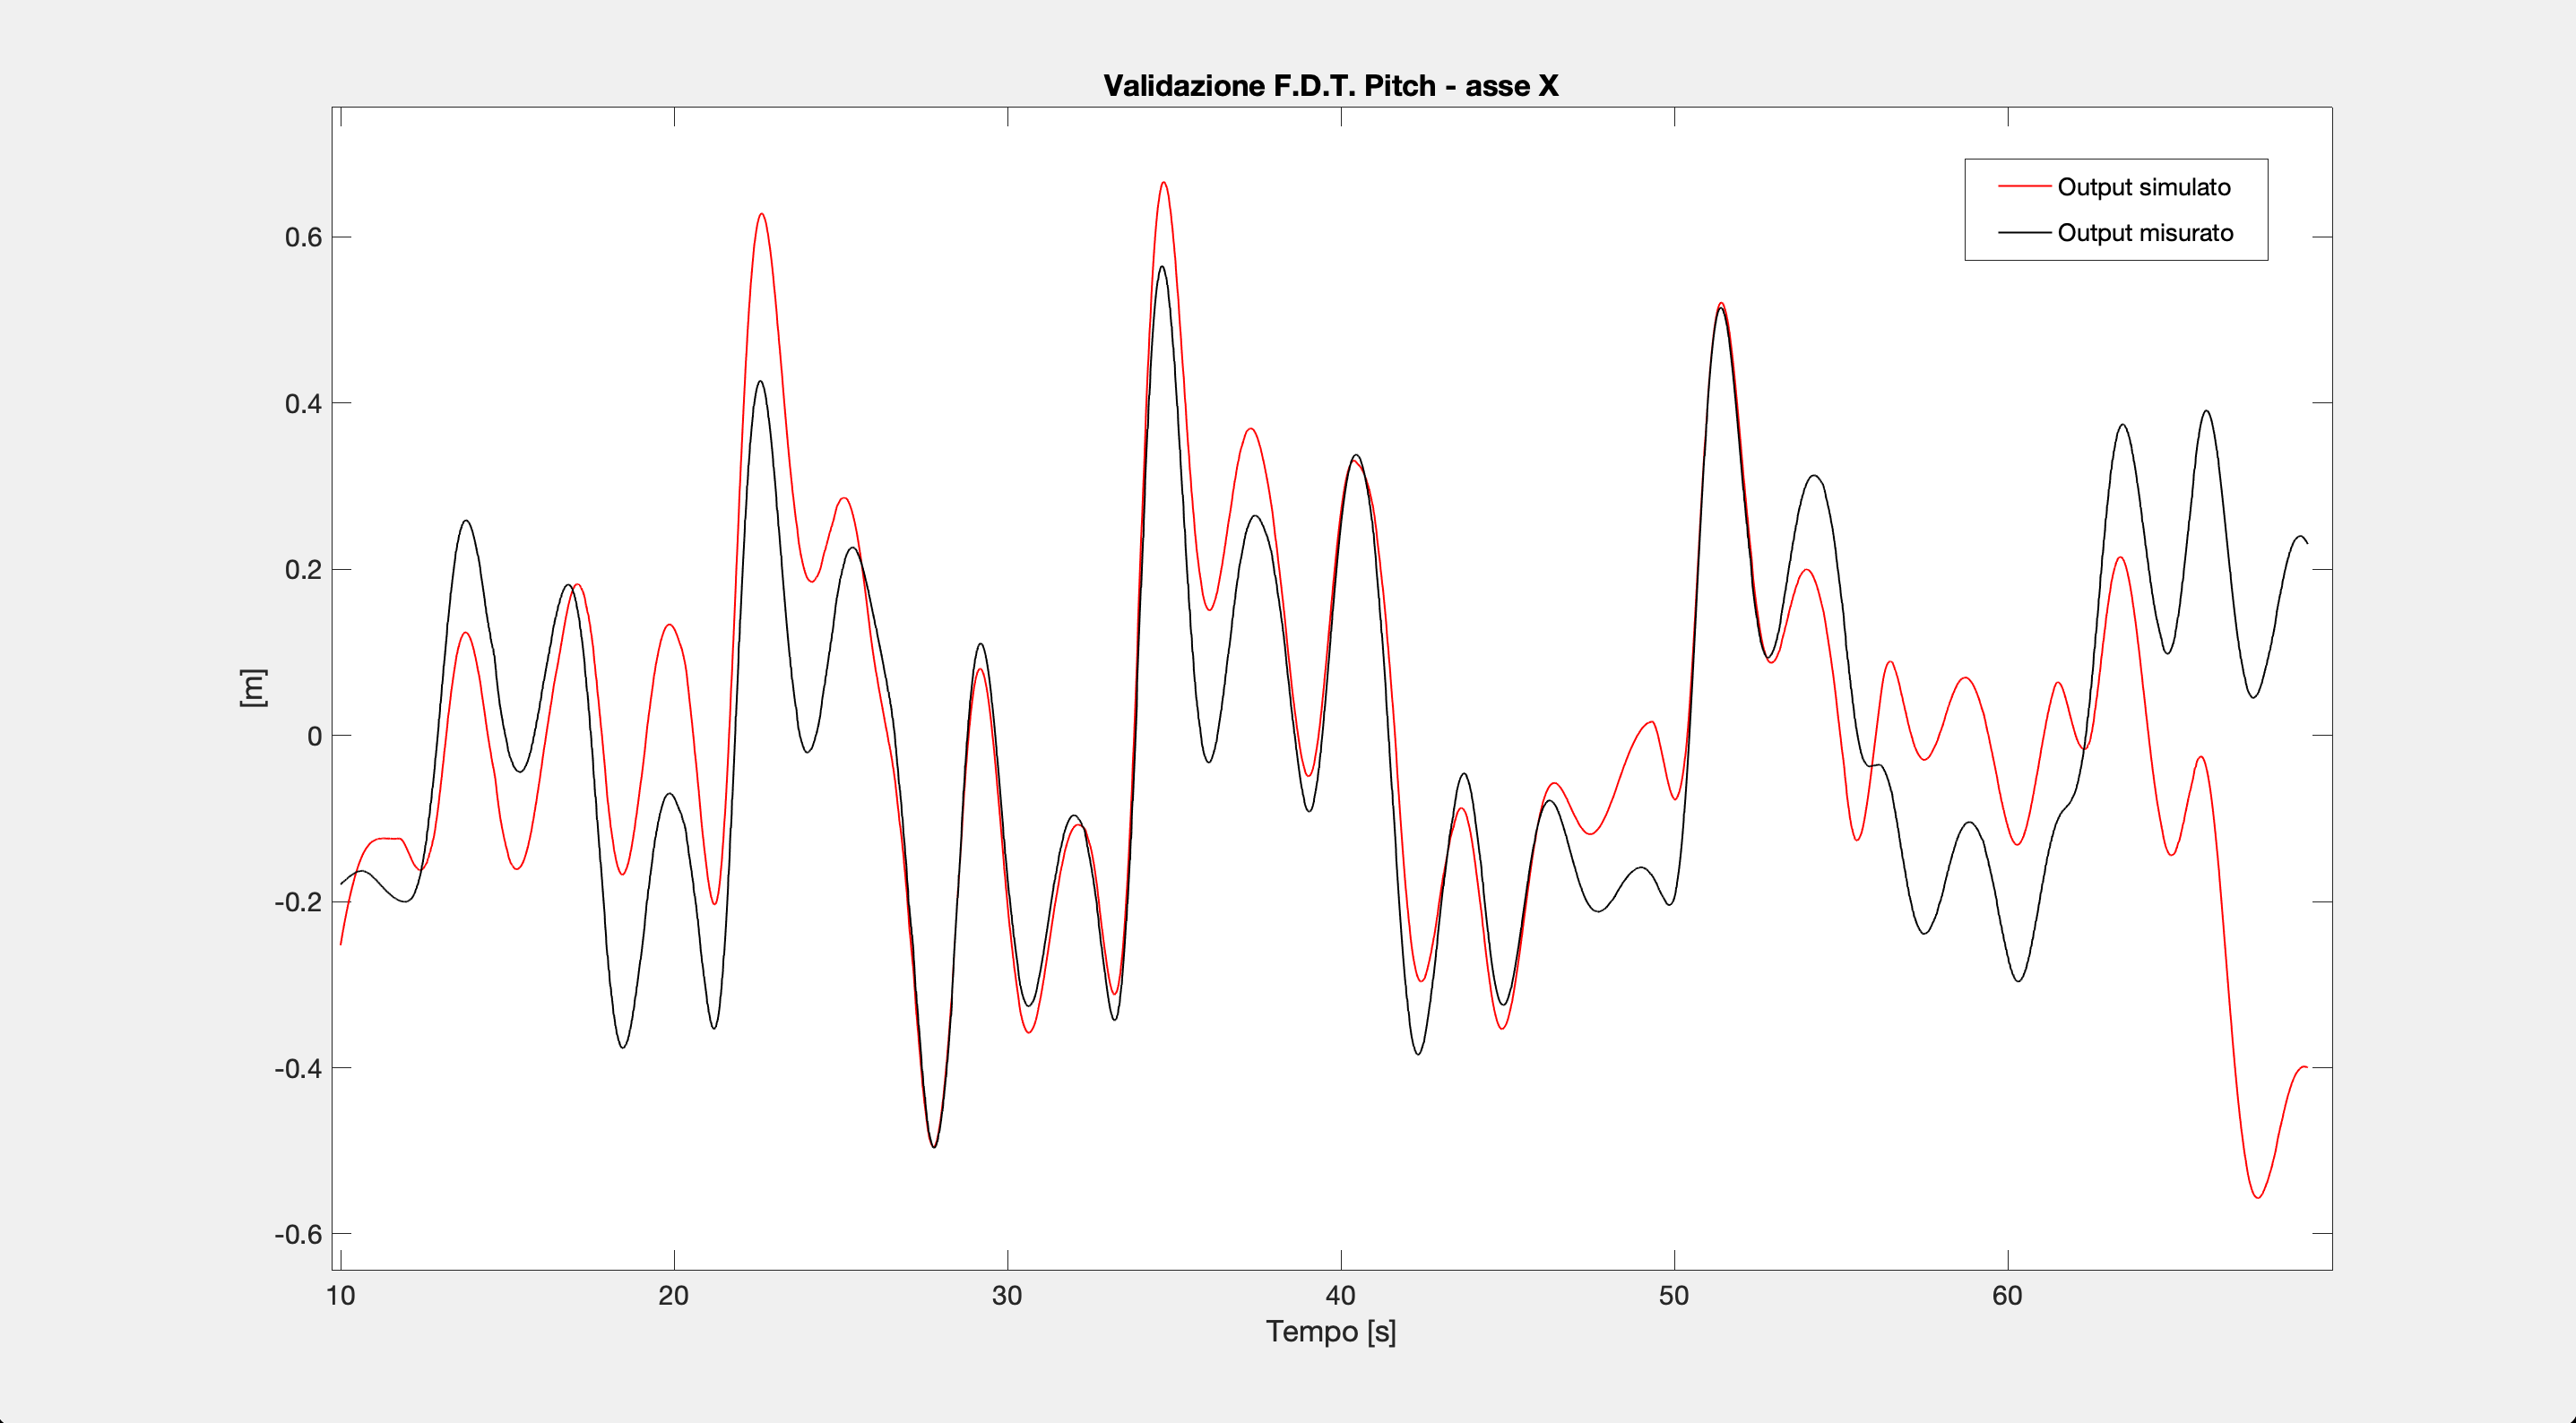
\includegraphics[width=1\textwidth]{gfx/SysId/px_model}
	\caption[Validazione F.D.T. Pitch - asse X.]{Validazione F.D.T. Pitch - asse X.}
	\label{fig:px_model}
\end{figure}

\subsection{Funzione di Trasferimento forza di Spinta e posizione lungo Z}
I dati utilizzati per identificare la dinamica del velivolo lungo l'asse Z sono il segnale che descrive le variazioni della forza di spinta (input) e il segnale che descrive le variazioni di posizione lungo lo stesso asse (output). Il drone subito dopo il decollo entra in stato di hovering, cioè rimane fisso sull'origine del piano XY ma ad una certa quota lungo l'asse Z. Questo significa che, a differenza dei due casi precedenti, in questo caso i segnali input-output non sono a media nulla. Pertanto, nel preprocessing si rendono entrambi a media nulla, come mostra Figura \ref{fig:tz_input}.\\

Il segnale di ingresso contenente le varie spinte applicate nel tempo è caratterizzato da una serie di gradini, di diversa ampiezza, in modo da evidenziare in maniera marcata il comportamento del sistema. Si è cercato di fare la stessa cosa per gli ingressi utilizzati nei casi precedenti, ma il meccanismo di stabilizzazione è risultato meno efficiente per spostamenti sul piano XY (rispetto a spostamenti lungo l'asse Z), ed è per questo che i segnali sono sicuramente più complicati da interpretare.

\begin{figure}[H]
	\centering
	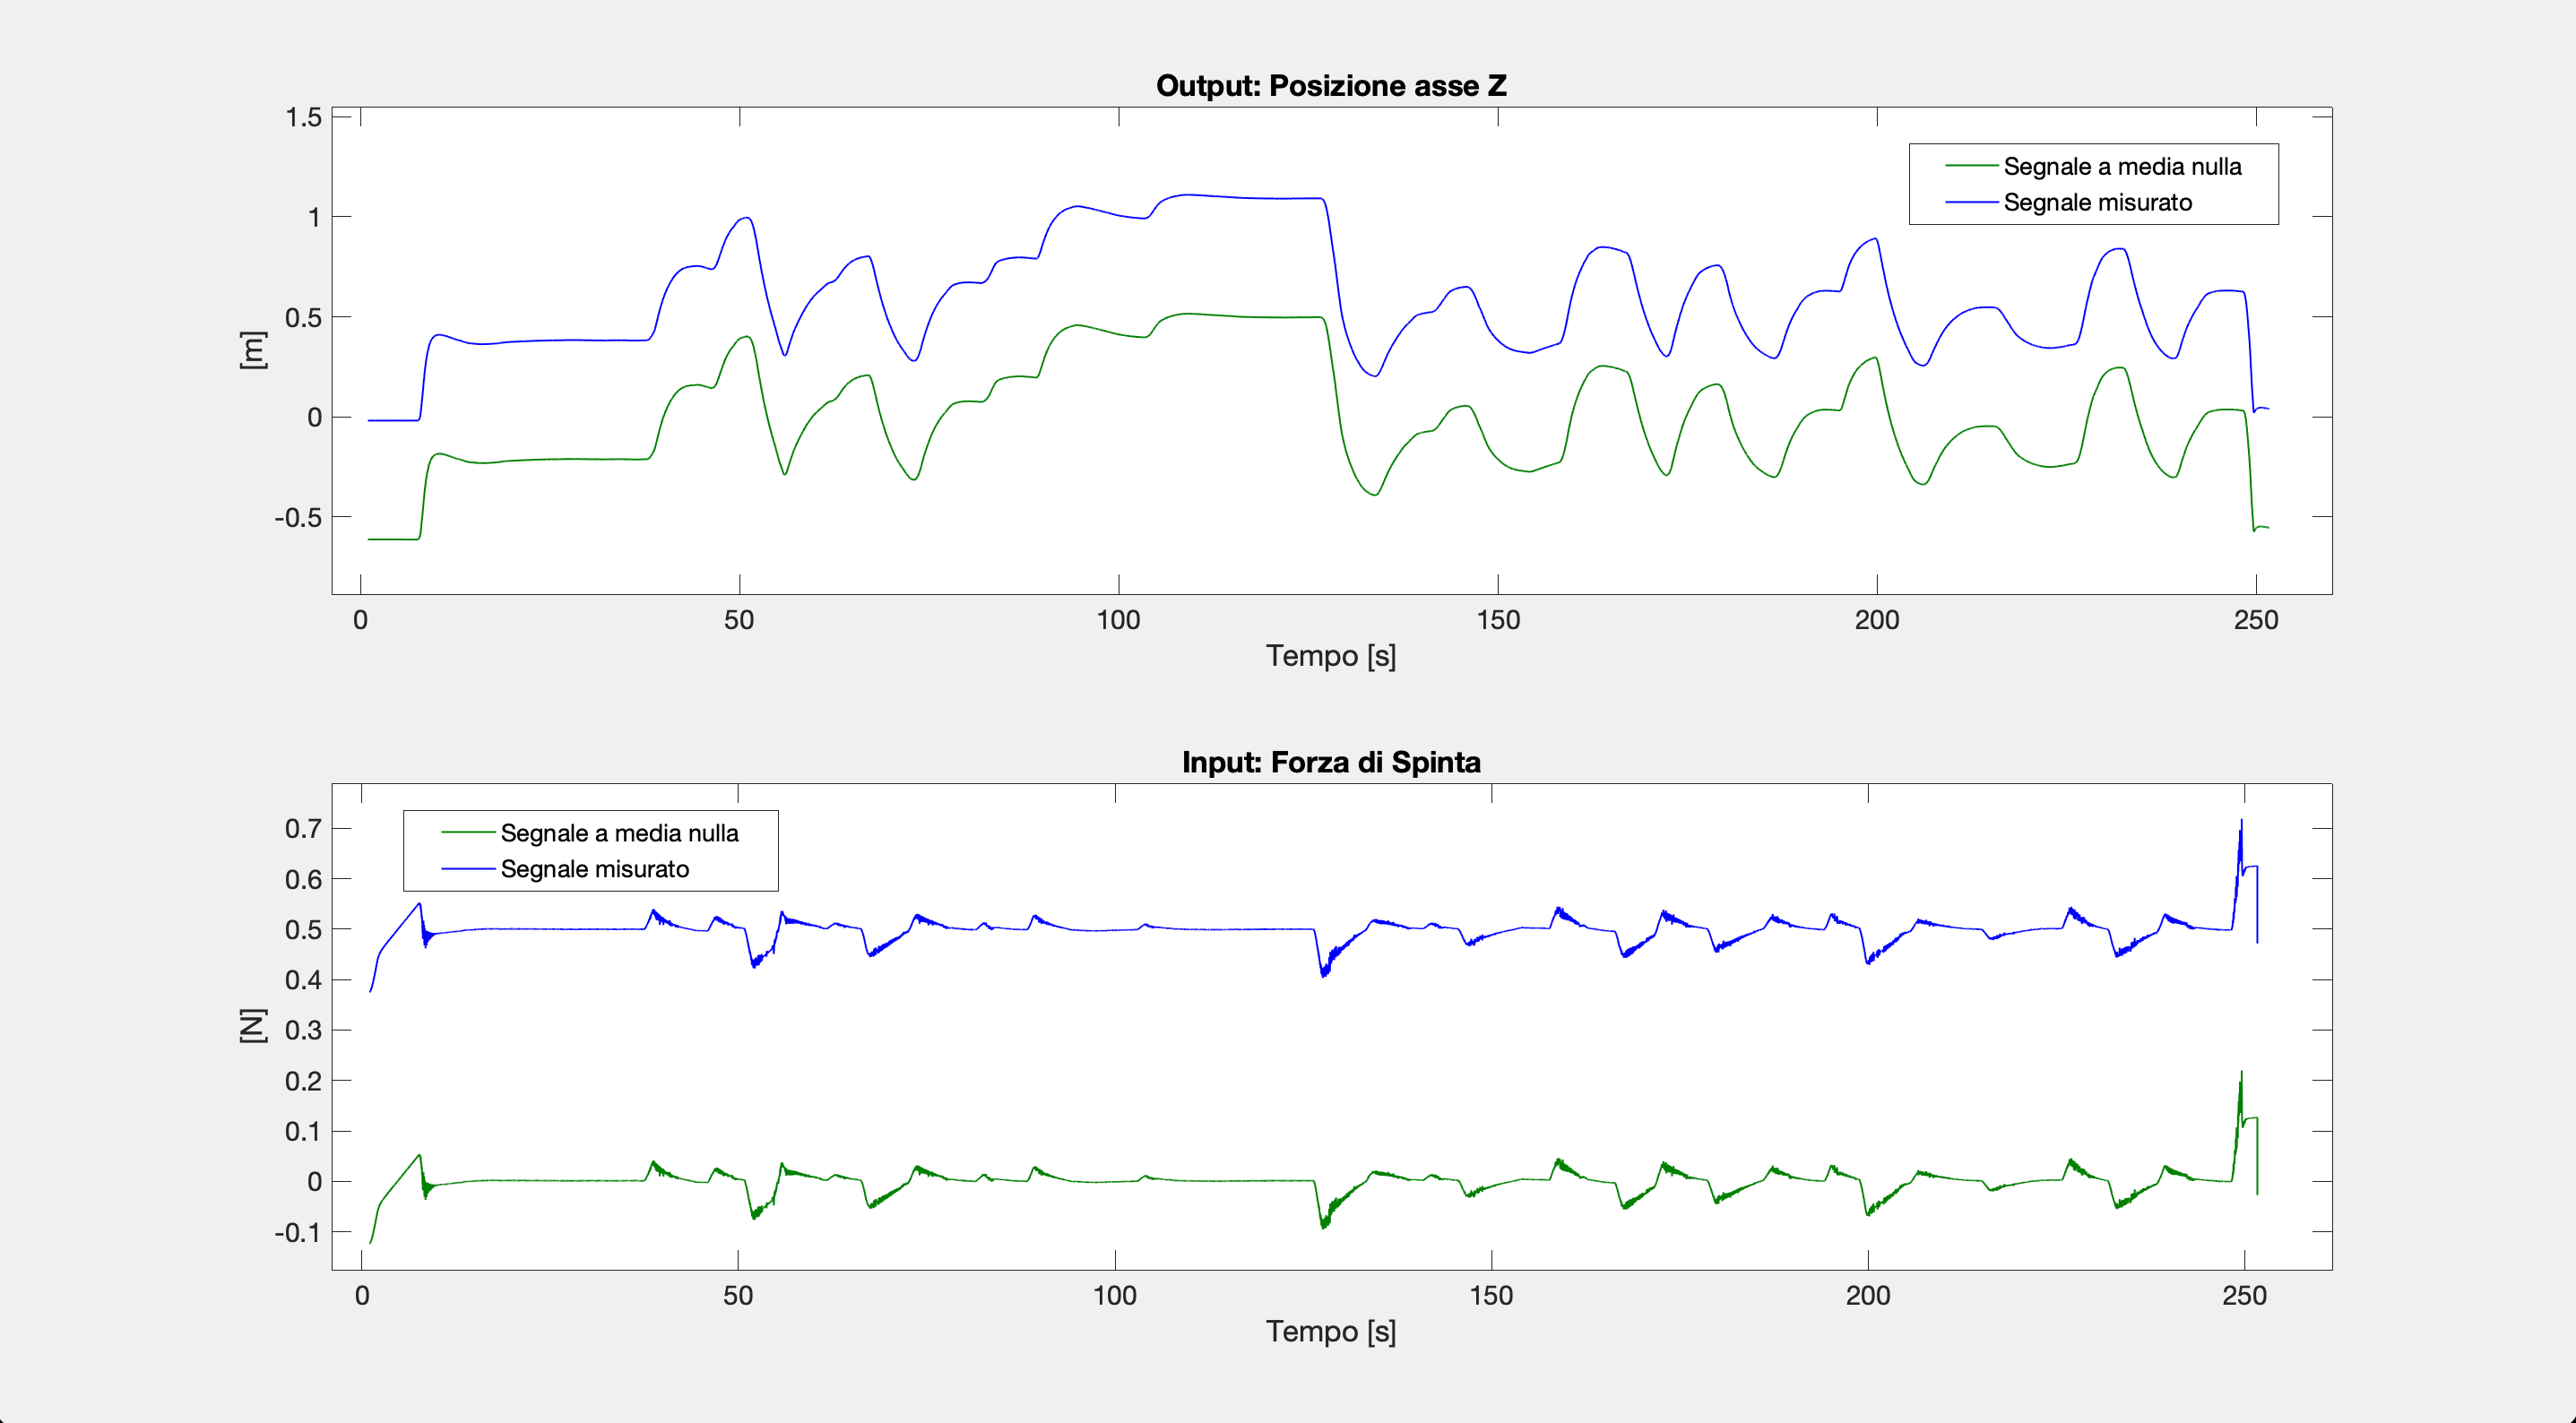
\includegraphics[width=1\textwidth]{gfx/SysId/tz_input}
	\caption[Dati input-output per identificare la dinamica della spinta.]{Dati input-output per identificare la dinamica della spinta. Input: forza di spinta applicata nel tempo. Output: variazione della posizione lungo l'asse Z nel tempo.}
	\label{fig:tz_input}
\end{figure}

La funzione di trasferimento identificata che lega la forza di spinta allo spostamento del velivolo lungo l'asse Z è la seguente (\ref{fdtZ}).

\begin{equation}
	W_Z(s) = \frac{-144s^2 + 97.89s + 25.18}{s^3 + 39.98s^2 + 12.35s + 0.7329}
	\label{fdtZ}
\end{equation}

Si ottiene ancora un sistema lineare tempo continuo del terzo ordine (tre poli).\\

Passando alla validazione, la funzione \emph{compare()} \cite{compare} mostra un'ottima compatibilità del modello identificato con quello reale, come mostra Figura \ref{fig:tz_model}. Il \acs{NRMSE} risulta in un 78.4\% di compatibilità.

\begin{figure}[H]
	\centering
	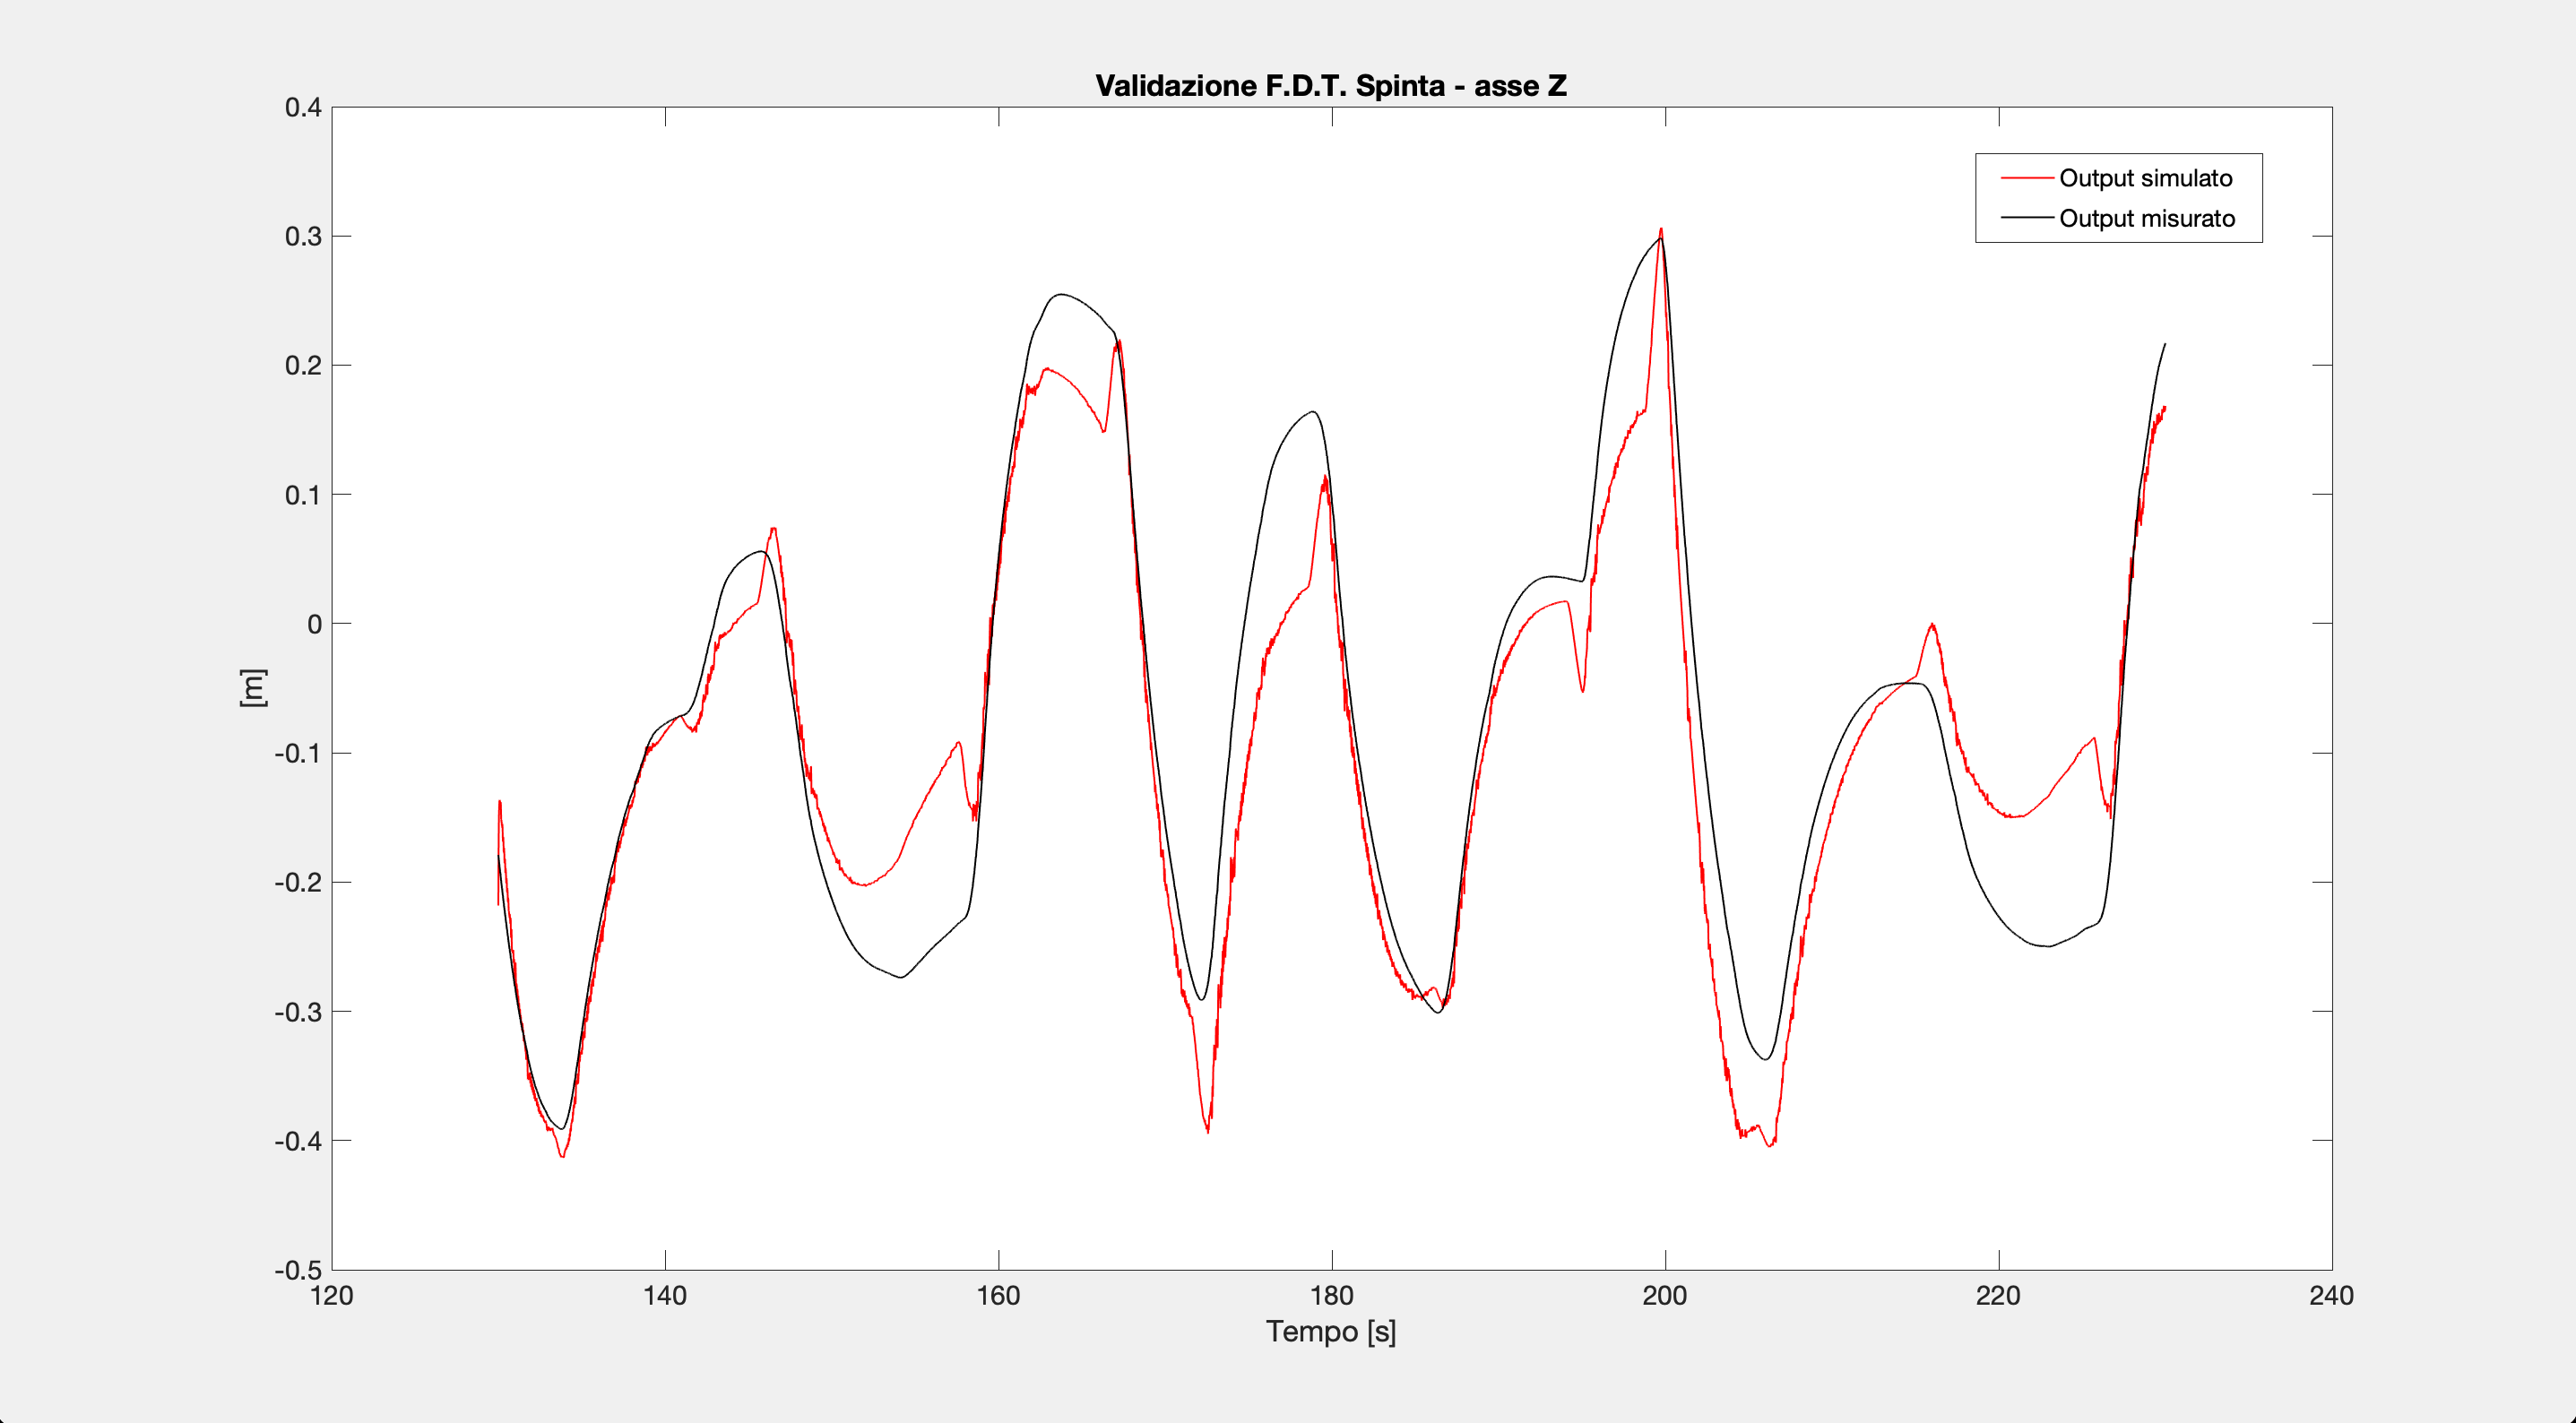
\includegraphics[width=1\textwidth]{gfx/SysId/tz_model}
	\caption[Validazione F.D.T. Spinta - asse Z.]{Validazione F.D.T. Spinta - asse Z.}
	\label{fig:tz_model}
\end{figure}

% ------------------------------ MIMO ------------------------------

\section{Identificazione Modello MIMO}


% CHAPTER 5

\chapter{Conclusioni}\label{ch:conc}


% BACK
\cleardoublepage% BIBLIOGRAPHY

\manualmark
\markboth{\spacedlowsmallcaps{\bibname}}{\spacedlowsmallcaps{\bibname}}

\refstepcounter{dummy}
\addtocontents{toc}{\protect\vspace{\beforebibskip}}
\addcontentsline{toc}{chapter}{\tocEntry{\bibname}}
\label{app:bibliography}
\printbibliography

% APPENDIX

\chapter*{Appendice}\label{ch:appendix}

Nel seguito si riportano le sezioni più significative del codice Python relativo al controllore di posizione (\emph{controller.py}). In particolare, le modifiche che sono state apportate per poter registrare e memorizzare i dati input-output di interesse.\\

\begin{lstlisting}[language=Python, numbers=none]
#! /usr/bin/env python3

import rospy
import numpy as np
from scipy import io as sio
import tf2_ros as tf2
from scipy.spatial.transform import Rotation as R

class Controller:

  def __init__(self):

    # INPUTS
    self.controller_roll = np.array([])
    self.controller_pitch = np.array([])
    self.controller_yaw = np.array([])
    self.controller_thrust = np.array([])

    # OUTPUTS
    self.pose_x = np.array([])
    self.pose_y = np.array([])
    self.pose_z = np.array([])

    # TRANSFORMS
    self.tf_buffer = tf2.Buffer()
    self.tf_listener = tf2.TransformListener(self.tf_buffer)
    try:
    transform = self.tf_buffer.lookup_transform(self.world_frame, self.drone_frame, rospy.Time(0), rospy.Duration(5))
    except tf2.LookupException:
    print("ERROR: No transformation between {} and {}.".format(self.world_frame, self.drone_frame))
    exit(-1)


    # POSE AND ORIENTATION (QUATERNION)
    self.init_pose = np.array([transform.transform.translation.x,
                                   transform.transform.translation.y,
                                   transform.transform.translation.z])
    self.init_orientation = np.array([transform.transform.rotation.x,
                               transform.transform.rotation.y,
                               transform.transform.rotation.z,
                               transform.transform.rotation.w])
    self.current_pose = copy.deepcopy(self.init_pose)
    self.current_orientation = copy.deepcopy(self.init_orientation)
  
  def _control_loop(self):
    while not self.kill_threads:
    
    # ROTATION MATRIX
    r = R.from_quat(current_orientation)
    current_rotation_matrix = np.array(r.as_matrix()).reshape((3, 3))

    if self.current_state != self.drone_states["GROUND"]:

      # REGISTRAZIONE OUTPUT (X,Y,Z)
      xp = np.append(self.pose_x, [current_pose[0]])
      self.pose_x = xp
      yp = np.append(self.pose_y, [current_pose[1]])
      self.pose_y = yp
      zp = np.append(self.pose_z, [current_pose[2]])
      self.pose_z = zp
      
      

      if not self.current_state == self.drone_states["FAIL"]:
         if not self.current_state == self.drone_states["TAKING_OFF"]:

            # CONTROLLO STABILIZZATO
            if self.angle_mode:

            # CALCOLO PHI, THETA, PSI, T

            # REGISTRAZIONE INPUT (PHI, THETA, PSI, T)
            r1 = np.append(self.controller_roll, [roll])
            self.controller_roll = r1
            p1 = np.append(self.controller_pitch, [pitch])
            self.controller_pitch = p1
            y1 = np.append(self.controller_yaw, [yaw])
            self.controller_yaw = y1
            t1 = np.append(self.controller_thrust, [trust])
            self.controller_thrust = t1

            self.publish_attitude_angle(roll, pitch, yaw, trust)

            # CONTROLLO ACROBATICO    
            else:
            self.publish_attitude_acro(wtr[0], wtr[1], wtr[2],
                    
        else: # TAKE OFF

          # CALCOLO PHI, THETA, PSI, T

          # REGISTRAZIONE INPUT (PHI, THETA, PSI, T)
          r2 = np.append(self.controller_roll, [roll])
          self.controller_roll = r2
          p2 = np.append(self.controller_pitch, [pitch])
          self.controller_pitch = p2
          y2 = np.append(self.controller_yaw, [yaw])
          self.controller_yaw = y2
          t2 = np.append(self.controller_thrust, [trust])
          self.controller_thrust = t2

          self.publish_attitude_angle(roll, pitch, yaw, trust)

    # DATA DICTIONARY        
    input_output_dic = {
    "controller_roll": self.controller_roll,
    "controller_pitch": self.controller_pitch,
    "controller_yaw": self.controller_yaw,
    "controller_thrust": self.controller_thrust,
    "pose_x": self.pose_x,
    "pose_y": self.pose_y,
    "pose_z": self.pose_z
    }

    # MATLAB
    sio.savemat("input_output_data.mat", input_output_dic)

    self.rate_pid.sleep()

if __name__ == "__main__":
    controller = Controller()
    while not rospy.is_shutdown():
        controller._control_loop()
\end{lstlisting}


\end{document}
